% !TeX spellcheck = en_GB_oxendict
\documentclass[11pt,a4paper]{article}
\usepackage[utf8]{inputenc}
\usepackage[T1]{fontenc}
\usepackage{amsmath,amssymb,makeidx,graphicx,float,indentfirst,color,hyperref,tikz,ifthen, fancyref,pgfplots,verbatim,fancyvrb,caption,subcaption,physics,longtable,mathrsfs, mathtools}
\usepackage{afterpage}
\newcommand\blankpage{%
	\null
	\thispagestyle{empty}%
	\addtocounter{page}{-1}
	\newpage}
\numberwithin{equation}{section}
\usepackage[width=15.00cm, height=23.00cm]{geometry}
\setlength{\parindent}{6mm}
\setlength{\parskip}{1mm}
\hypersetup{colorlinks=true, linktoc=all, linkcolor=blue,}
\pgfplotsset{compat=1.15}
%\usepgfplotslibrary{groupplots,dateplot,arrows}
\usetikzlibrary{patterns,shapes.arrows}
\usepackage{listings,xcolor}
\definecolor{codegreen}{rgb}{0,0.6,0}
\definecolor{codegray}{rgb}{0.5,0.5,0.5}
\definecolor{codepurple}{rgb}{0.58,0,0.82}
\definecolor{backcolour}{rgb}{0.95,0.95,0.92}
\lstdefinestyle{mystyle}{
	backgroundcolor=\color{backcolour},   
	commentstyle=\color{codegreen},
	keywordstyle=\color{magenta},
	numberstyle=\tiny\color{codegray},
	stringstyle=\color{codepurple},
	basicstyle=\ttfamily\footnotesize,
	breakatwhitespace=false,         
	breaklines=true,                 
	captionpos=b,                    
	keepspaces=true,                 
	numbers=left,                    
	numbersep=5pt,                  
	showspaces=false,                
	showstringspaces=false,
	showtabs=true,                  
	tabsize=2,
}
\lstset{style=mystyle}
%----------------------------------------------------------------------

\author{Pritish Karmakar}

\begin{document}
	\begin{titlepage}
		\vspace*{1cm}
		\centering
		{\Huge\bfseries Summer Internship Report}\\
		\vspace{1cm}
		{\LARGE Indian Institution of Science Education \& Research}\\
		\vspace{3.5mm}
		{\LARGE Kolkata, WB, India, 741246}\\
		\vspace{5mm}
		
		
\includegraphics[width=4cm]{iiserk.png}
		\vfill
		\textbf{\textsc{\LARGE 
				On Polarization Properties of Light,\\\vspace{2mm}
				Gaussian Beams and Spin-Orbit Interaction.}}\\
		
		\vspace{15mm}
		
		\textsl{\LARGE Submitted by}\\\vspace{2mm}
		\textbf{\huge Pritish Karmakar}\\\vspace{1.5mm}
		{\LARGE (21MS179)}\\
		\vspace{10mm}
		
		\textsl{\LARGE Submitted to}\\\vspace{3mm} 
		\textbf{\huge Prof. Ayan Banerjee}\\\vspace{1.5mm}
		{\LARGE (HOD, DPS, IISER Kolkata)}\\
		\vspace{10mm}
		
		\textsl{\LARGE Dated}\\\vspace{3mm} 
		\textbf{\huge17.05.23 - 20.07.23}\\
		\vspace{1cm}
		\clearpage
		
		\iffalse
		\newpage 
		\thispagestyle{empty}
		\begin{center}
			This page is intentionally left blank
		\end{center}
		\newpage
		\fi
		
		\iffalse
		\parindent=0pt
		\thispagestyle{empty}
		\begin{center}
			\slshape
			
			
			\vspace*{\fill}
			\color{darkgray}{\Large{\textbf{“} Nobody ever figures out what life is all about, and it\\ doesn't matter. Explore the world. Nearly everything\\ is really interesting if you go into it deeply enough. \textbf{”}} \par} 
			\vspace{8mm}
			\textsc{\Large \textbf{Richard P. Feynman}}
			\vspace*{\fill}
			
		\end{center}
		\clearpage
		\fi
		
		\newpage 
		
		\thispagestyle{empty}
		{\centering\Huge\bfseries Acknowledgement}
		\vspace{12mm}
		\begin{flushleft}
		\Large
		\hspace{7mm}I am incredibly grateful to have had the opportunity to work on a fascinating summer project on the topic of optics under  \textbf{Prof. Ayan Banerjee}\footnote{HOD, Department of Physical Sciences, IISER Kolkata, Room No: M-130, email: \href{mailto:ayan@iiserkol.ac.in}{ayan@iiserkol.ac.in}} and with the mentorship of \textbf{Ram Nandan Kumar}\footnote{Int. PhD, Department of Physical Sciences, IISER Kolkata, email: \href{mailto:ramnandan899@gmail.com}{ramnandan899@gmail.com}}. This project has been an enriching and enlightening experience for me, and I am indebted to the support and expertise provided by both of them.  The project was a reading-oriented project of duration from the 17th of May to the 20th of July of 2023, and throughout this period, {Prof. Ayan Banerjee} and {Ram Nandan Kumar} extended their unwavering support, sharing their valuable insights and encouraging me to deepen my understanding of the subject matter.\\
		\vspace{5mm}
		\hspace{7mm}Finally, I want to thank my family and friends for their unwavering support and understanding throughout this journey. Their encouragement provided the motivation I needed to stay focused and determined.\\
		\vspace{5mm}
		\hspace{7mm}In conclusion, I feel immensely fortunate to have worked on this summer project and the knowledge and experiences gained during this period will undoubtedly shape my academic and professional pursuits in the future.\\
		\vspace{5mm}
		\hspace{7mm}Thank you all for being an integral part of this enriching journey.\\
		\vspace{5mm}
		Sincerely,\\
		\vspace{5mm}
		\textit{\LARGE Pritish Karmakar}\\
		\textit{20.07.23} 
		\end{flushleft}
		\newpage
		
		
		\pagenumbering{roman}
		
		\tableofcontents
		\clearpage
		\listoffigures
		\listoftables
		%\lstlistoflistings
		
	\end{titlepage}

\pagenumbering{arabic}

\section{POLARIZATION}
\subsection{Introduction}
We know, in EM wave, the electric field and magnetic field oscillating perpendicularly in the transverse plane \textit{w.r.t.} the propagation direction. \textit{Polarization} is the property of an EM wave, which deals with the temporal and spatial variation of the orientation of field vector (mainly,  electric field) of the EM wave. Here we mainly discuss Jones formalism, Stokes-Muller formalism and finally apply those thing in elliptically polarized light.

\subsection{Jones formalism}
\subsubsection{Jones Vector}
Vector form of electric field of fully polarized EM wave propagating along z-axis is given by
\begin{align}
	\boldsymbol{E}(\boldsymbol{x},t)=
	\begin{bmatrix}
		E_x(\boldsymbol{x},t)\\
		E_y(\boldsymbol{x},t)\\
		E_z(\boldsymbol{x},t)
	\end{bmatrix} =
\begin{bmatrix}
	A_x(\boldsymbol{x}) e^{-i(kz-\omega t-\delta_x)}\\
	A_y(\boldsymbol{x}) e^{-i(kz-\omega t-\delta_y)}\\
	0
\end{bmatrix}=
\begin{bmatrix}
	A_x(\boldsymbol{x})e^{i\delta_x}\\
	A_y(\boldsymbol{x})e^{i\delta_y}\\
	0
\end{bmatrix}e^{-i(kz-\omega t)}
\end{align}

We define normalized\footnote{normalized as $\boldsymbol{J}^\ast\:\boldsymbol{J}=1$} \textit{Jones vector} as
\begin{align}
	\boldsymbol{J}(\boldsymbol{x},t)=\frac{1}{\sqrt{A_x^2+A_y^2}}
	\begin{bmatrix}
		A_x(\boldsymbol{x})e^{i\delta_x}\\
		A_y(\boldsymbol{x})e^{i\delta_y}
	\end{bmatrix}
\end{align}

Such examples of usual polarization states are given below \cite{jones},
\begin{table}[H]
	\centering
	\begin{tabular}{ c c } 
		\hline
		\hline
		Polarization state & $\boldsymbol{J}$\\
		\hline
		$\ket{H}$ & $\begin{bmatrix}1\\0\end{bmatrix}$ \\ \hline
		$\ket{V}$ & $\begin{bmatrix}0\\1\end{bmatrix}$ \\ \hline
		$\ket{P}$ & $\frac{1}{\sqrt{2}}\begin{bmatrix}1\\1\end{bmatrix}$ \\ \hline
		$\ket{M}$ & $\frac{1}{\sqrt{2}}\begin{bmatrix}1\\-1\end{bmatrix}$ \\ \hline
		$\ket{L}$ & $\frac{1}{\sqrt{2}}\begin{bmatrix}1\\i\end{bmatrix}$ \\ \hline
		$\ket{R}$ & $\frac{1}{\sqrt{2}}\begin{bmatrix}1\\-i\end{bmatrix}$ \\ 
		\hline
		\hline
	\end{tabular}
	\caption{Jones vector of usual polarization state}
	\label{table:1}
\end{table}

Some properties of Jones vector are
\begin{enumerate}
	\item The intensity of the EM wave is given by 
	\begin{align}
		I= \frac{1}{2}c\epsilon_0(A_x^2+A_y^2) = \frac{1}{2}c\epsilon_0 (\boldsymbol{E}^\ast \boldsymbol{E})= \frac{1}{2}c\epsilon_0 (\boldsymbol{J}^\ast \boldsymbol{J})
	\end{align}
	\item For general elliptically polarized light we can measure the azimuth ($\alpha$) ellipticity ($\epsilon$) of the polarization ellipse by comparing Jones vector $\boldsymbol{J}$ with \cite{WO}
	\begin{align*}
		\begin{bmatrix}
			\cos\alpha\cos\epsilon- i \sin\alpha\sin\epsilon \\
			\sin\alpha\cos\epsilon+ i \cos\alpha\sin\epsilon
		\end{bmatrix}
	\end{align*}
\end{enumerate}

\subsubsection{Jones Matrix \& evolution of Jones vector}
\textit{Jones matrix} is a $2\times2$ matrix assigned for a particular optical element. Let $\boldsymbol{M}$ be the Jones matrix for an optical element \textit{s.t.} 
\begin{align*}\boldsymbol{M}=
	\begin{bmatrix}
		m_{11} & m_{12}\\
		m_{21} & m_{22}
	\end{bmatrix}
\end{align*}
then if a polarized light of Jones vector $\boldsymbol{J}_{in}$ passes through that optical element then the Jones vector of output light is given by 
\begin{align}
	\boldsymbol{J}_{out}&=\boldsymbol{M}\;\boldsymbol{J}_{in}\label{eq:1.4}\\	\Rightarrow \boldsymbol{E}_{out}&=\boldsymbol{M}\;\boldsymbol{E}_{in} \label{eq:1.5}
\end{align}

To determine $m_{ij}$ in $\boldsymbol{M}$,
\begin{enumerate}
	\item Pass x-polarized light and determine $\boldsymbol{J}_{out}$, then 
	\begin{align*}
		\boldsymbol{J}_{out}=
		\begin{bmatrix}
			m_{11} & m_{12}\\
			m_{21} & m_{22}
		\end{bmatrix}
		\begin{bmatrix}
			1\\
			0
		\end{bmatrix}=
	\begin{bmatrix}
		m_{11}\\
		m_{21}
	\end{bmatrix}
	\end{align*}

\item Pass y-polarized light and determine $\boldsymbol{J}_{out}$, then 
\begin{align*}
	\boldsymbol{J}_{out}=
	\begin{bmatrix}
		m_{11} & m_{12}\\
		m_{21} & m_{22}
	\end{bmatrix}
	\begin{bmatrix}
		0\\
		1
	\end{bmatrix}=
	\begin{bmatrix}
		m_{12}\\
		m_{22}
	\end{bmatrix}
\end{align*}
\end{enumerate}

Such examples of usual Jones matrix \footnote{For polariser the Jones matrix $\boldsymbol{M} = \boldsymbol{J}\;\boldsymbol{J}^\ast$ where $\boldsymbol{J}$ is normalized Jones vector corresponding polarization state \textit{s.t.} $\boldsymbol{J}_{out}= \boldsymbol{M}\boldsymbol{J} = (\boldsymbol{J}\boldsymbol{J}^\ast)\boldsymbol{J}=\boldsymbol{J}(\boldsymbol{J}^\ast\boldsymbol{J})=\boldsymbol{J}$ \label{fn:1}} are given below,\cite{jones}

\begin{longtable}[H]{ c c } 
	\hline
	\hline
	Optical element & $\boldsymbol{M}$\\
	\hline\endhead
	Free space & $\begin{bmatrix}
		1 & 0 \\ 
		0 & 1
	\end{bmatrix}$\\ \hline
	x-Polariser & $\begin{bmatrix}
		1 & 0 \\ 
		0 & 0
	\end{bmatrix}$\\\hline
	y-Polariser & $\begin{bmatrix}
		0 & 0 \\ 
		0 & 1
	\end{bmatrix}$\\\hline
	Right circular polariser & $\frac{1}{2}\begin{bmatrix}
		1 & i \\ 
		-i & 1
	\end{bmatrix}$\\\hline
	Left circular polariser & $\frac{1}{2}\begin{bmatrix}
		1 & -i \\ 
		i & 1
	\end{bmatrix}$\\\hline
	Linear di-attenuator & $\begin{bmatrix}
		a & 0 \\ 
		0 & b
	\end{bmatrix}$\\\hline
	\begin{tabular}{c}
		Half-wave plate\\
		with fast axis horizontal
	\end{tabular} & $e^{-i\pi/2}\begin{bmatrix}
		1 & 0 \\ 
		0 & -1
	\end{bmatrix}$\\\hline
	\begin{tabular}{c}
		Quarter-wave plate\\
		with fast axis horizontal
	\end{tabular} & $e^{-i\pi/4}\begin{bmatrix}
		1 & 0 \\ 
		0 & i
	\end{bmatrix}$\\\hline
	General phase retarder &  $\begin{bmatrix}
		e^{i\phi_x} & 0 \\ 
		0 & e^{i\phi_y}
	\end{bmatrix}$\\
\hline
\hline
\caption{Jones matrix related to usual optical element}
\label{table:2}
\end{longtable}



Some properties of Jones matrix are 
\begin{enumerate}
	\item Resultant Jones matrix for composition of $n$ optical elements is given by
	\begin{align}
		\boldsymbol{M}=\boldsymbol{M}_1\;\boldsymbol{M}_2\dots\boldsymbol{M}_n
	\end{align}
	\item For an optical element when its optical axis aligned at an angle $\theta$ \textit{w.r.t.} x-axis then resultant Jones matrix for this rotated optical element is given by
	\begin{align}
		\boldsymbol{M}_\theta = R(-\theta)\;\boldsymbol{M}\;R(\theta) \label{eq:1.7}
	\end{align}
where $R(\theta)$ is passive rotation matrix \textit{s.t.}
\begin{align}
	R(\theta)=
	\begin{bmatrix}
		\cos\theta & \sin\theta \\
		-\sin\theta & \cos\theta
	\end{bmatrix}
\end{align}
\end{enumerate}

\subsubsection{Drawback of Jones formalism}
Main drawback of Jones formalism is that its application is restricted in fully polarized light. This formalism cannot explain the partially polarized or unpolished light which we frequently observe in practical use.
\subsection{Stokes-Muller formalism}
\subsubsection{Coherency matrix}
\textit{Coherency matrix} of a EM wave is defined as \cite{WO} 
\begin{align}
	\boldsymbol{C}=\expval{\boldsymbol{E}\otimes\boldsymbol{E}^\dagger}= \expval{\boldsymbol{E}\boldsymbol{E}^\dagger}=
	\begin{bmatrix}
		\expval{E_xE_x^\ast} & \expval{E_xE_y^\ast}\\
		\expval{E_yE_x^\ast} & \expval{E_yE_y^\ast}
	\end{bmatrix}=
\begin{bmatrix}
	c_{xx} & c_{xy}\\
	c_{yx} & c_{yy}
\end{bmatrix}\label{coherency matrix}
\end{align}
where $\otimes$ denotes Kronecker product and $\expval{\cdot}$ denotes the temporal avg of the corresponding quantity.

Examples of coherency matrix of usual polarization states are given below \cite{coherency},
\begin{table}[H]
	\centering
	\begin{tabular}{ c c c } 
		\hline
		\hline
		Polarization state & $\boldsymbol{J}$ & $\boldsymbol{C}$\\
		\hline
		$\ket{H}$ & $\begin{bmatrix}1\\0\end{bmatrix}$ & $\begin{bmatrix}1&0\\0&0\end{bmatrix}$\\ \hline
		$\ket{V}$ & $\begin{bmatrix}0\\1\end{bmatrix}$ & $\begin{bmatrix}0&0\\0&1\end{bmatrix}$\\ \hline
		$\ket{P}$ & $\frac{1}{\sqrt{2}}\begin{bmatrix}1\\1\end{bmatrix}$ & $\frac{1}{2}\begin{bmatrix}1&1\\1&1\end{bmatrix}$\\ \hline
		$\ket{M}$ & $\frac{1}{\sqrt{2}}\begin{bmatrix}1\\-1\end{bmatrix}$ & $\frac{1}{2}\begin{bmatrix}1&-1\\-1&1\end{bmatrix}$\\ \hline
		$\ket{L}$ & $\frac{1}{\sqrt{2}}\begin{bmatrix}1\\i\end{bmatrix}$ & $\frac{1}{2}\begin{bmatrix}1&-i\\i&1\end{bmatrix}$\\ \hline
		$\ket{R}$ & $\frac{1}{\sqrt{2}}\begin{bmatrix}1\\-i\end{bmatrix}$ & $\frac{1}{2}\begin{bmatrix}1&i\\-i&1\end{bmatrix}$\\ \hline
		Un-polarized & $-$ &  $\frac{1}{2}\begin{bmatrix}1&0\\0&1\end{bmatrix}$\\
		\hline
		\hline
	\end{tabular}
	\caption{Coherency matrix of usual polarization state}
	\label{table:3}
\end{table}


Some properties of coherency matrix are
\begin{enumerate}
	\item It is a hermitian matrix \textit{i.e.} $\boldsymbol{C}=\boldsymbol{C}^\dagger$
	\item Trace and determinant off the matrix are non-negative \textit{i.e.} $\tr(\boldsymbol{C})>0$ \& $\det(\boldsymbol{C})\ge0$.
	\item $\Tr(\boldsymbol{C}) = \expval{E_x E_x^\ast} +\expval{E_y E_y^\ast}$ is the time averaged intensity of input light.
	\item let the polarized light (of electric field $\boldsymbol{E}_{in}$ \& coherency matrix $\boldsymbol{C}_{in}$) passes through an optical element (of Jones matrix $\boldsymbol{M}$) then let output electric field be $\boldsymbol{E}_{out}$ by the equation \ref{eq:1.5}, then output coherency matrix $\boldsymbol{C}_{out}$ is given by 
	\begin{align}
		\boldsymbol{C}_{out} = \expval{\boldsymbol{E}_{out}\boldsymbol{E}_{out}^\dagger} &= \expval{\left(\boldsymbol{M}\boldsymbol{E}_{in} \right) \left(\boldsymbol{M}\boldsymbol{E}_{in}\right)^\dagger}\nonumber\\
		&= \expval{\left(\boldsymbol{M}\boldsymbol{E}_{in} \right) \left(\boldsymbol{E}_{in}^\dagger\boldsymbol{M}^\dagger\right)}\nonumber \\
		&= \boldsymbol{M}\expval{\boldsymbol{E}_{in} \boldsymbol{E}_{in}^\dagger}\boldsymbol{M}^\dagger \nonumber\\
		&= \boldsymbol{M}\:\boldsymbol{C}_{in}\:\boldsymbol{M}^\dagger \label{eq:1.10}
	\end{align}
\end{enumerate}

\subsubsection{Stokes parameters and Stokes vector}
Now we see that coherency matrix $\boldsymbol{C}$ of any polarization state in table \ref{table:3} can be written in the linear combination of the 4 basis given below \cite{yt video}
\begin{align}
	\beta = \left\{
	\underbrace{\begin{bmatrix}1 & 0 \\ 0 & 1\\\end{bmatrix}}_{\boldsymbol{V_0}},
	\underbrace{\begin{bmatrix}1 & 0 \\ 0 & -1\\\end{bmatrix}}_{\boldsymbol{V_1}},
	\underbrace{\begin{bmatrix}0 & 1 \\ 1 & 0\\\end{bmatrix}}_{\boldsymbol{V_2}},
	\underbrace{\begin{bmatrix}0 & i \\ -i & 0\\\end{bmatrix}}_{\boldsymbol{V_3}}
	\right\}
\end{align}
Now we can write any coherency matrix $ \boldsymbol{C} $ as 
\begin{align}
\boldsymbol{C} = \frac{1}{2} \sum_{i=0}^{3} S_i \boldsymbol{V_i} \label{eq:1.12}
\end{align}
Note that all $V_i$'s are Hermitian, so obviously is $ \boldsymbol{C} $.

We call $\{S_0, S_1, S_2, S_3\}$ as a \textit{Stokes parameter} and the values of $S_i$'s are experimentally measurable.

A \textit{Stokes vector} $ \boldsymbol{S} $ is defined as\footnote{for intensity normalised Stokes vector, $\boldsymbol{s}= \begin{bmatrix} 1& s_1& s_2& s_3\end{bmatrix}$ where $s_i=S_i/S_0$}

\begin{align}
	\boldsymbol{S}= \begin{bmatrix} S_0\\ S_1\\ S_2\\S_3\end{bmatrix}
\end{align}

Examples of Stokes vector for different polarization states are given below
\begin{table}[H]
	\centering
	\begin{tabular}{ c c c } 
		\hline
		\hline
		Polarization state &  $\boldsymbol{C}$ & $\boldsymbol{S}$\\
		\hline
		$\ket{H}$ & $\begin{bmatrix}1&0\\0&0\end{bmatrix}$ & $\begin{bmatrix}1&1&0&0\end{bmatrix}^T$\\ \hline
		$\ket{V}$ & $\begin{bmatrix}0&0\\0&1\end{bmatrix}$ & $\begin{bmatrix}1&-1&0&0\end{bmatrix}^T$\\ \hline
		$\ket{P}$ & $\frac{1}{2}\begin{bmatrix}1&1\\1&1\end{bmatrix}$ & $\begin{bmatrix}1&0&1&0\end{bmatrix}^T$\\ \hline
		$\ket{M}$ & $\frac{1}{2}\begin{bmatrix}1&-1\\-1&1\end{bmatrix}$ & $\begin{bmatrix}1&0&-1&0\end{bmatrix}^T$\\ \hline
		$\ket{L}$ & $\frac{1}{2}\begin{bmatrix}1&-i\\i&1\end{bmatrix}$ & $\begin{bmatrix}1&0&0&1\end{bmatrix}^T$\\ \hline
		$\ket{R}$ & $\frac{1}{2}\begin{bmatrix}1&i\\-i&1\end{bmatrix}$ & $\begin{bmatrix}1&0&0&-1\end{bmatrix}^T$\\ \hline
		Un-polarized &  $\frac{1}{2}\begin{bmatrix}1&0\\0&1\end{bmatrix}$ & $\begin{bmatrix}1&0&0&0\end{bmatrix}^T$\\
		\hline
		\hline
	\end{tabular}
	\caption{Stokes vector of usual polarization state}
	\label{table:4}
\end{table}
Note that all Jones vectors has Stokes vectors but converse need not to be true.

Now we see from the equation \ref{eq:1.12}
\begin{align}
	\begin{bmatrix}
		\expval{E_xE_x^\ast} & \expval{E_xE_y^\ast}\\
		\expval{E_yE_x^\ast} & \expval{E_yE_y^\ast}
	\end{bmatrix}=
	\boldsymbol{C} = \frac{1}{2} \sum_{i=0}^{3} S_i \boldsymbol{V_i} = \frac{1}{2}
	\begin{bmatrix}
		S_0+S_1 & S_2+iS_3\\
		S_2-iS_3 & S_0-S_1
	\end{bmatrix}
\end{align}
From there we can write
\begin{align}
	\boldsymbol{S}= \begin{bmatrix} S_0\\ S_1\\ S_2\\S_3\end{bmatrix} =
	\begin{bmatrix}
		\expval{E_xE_x^\ast} + \expval{E_yE_y^\ast}\\
		\expval{E_xE_x^\ast} - \expval{E_yE_y^\ast}\\
		\expval{E_yE_x^\ast} + \expval{E_xE_y^\ast}\\
		i\left(\expval{E_yE_x^\ast} - \expval{E_xE_y^\ast}\right)
	\end{bmatrix} \label{eq:1.15}
\end{align}

Now for a polarized light, 
\begin{align}
	\boldsymbol{C}=
	\begin{bmatrix}
		\expval{A_x^2} & \expval{A_xA_ye^{-i\delta}}\\
		\expval{A_xA_ye^{i\delta}} & \expval{A_y^2}
	\end{bmatrix} \text{ and }
	\boldsymbol{S}= \begin{bmatrix} S_0\\ S_1\\ S_2\\S_3\end{bmatrix} =
	\begin{bmatrix}
		\expval{A_x^2 + A_y^2}\\
		\expval{A_x^2 - A_y^2}\\
		\expval{2A_xA_y\cos\delta}\\
		\expval{2A_xA_y\sin\delta}
	\end{bmatrix} \label{eq:1.16}
\end{align}
where $\delta= \delta_y-\delta_x$.
\subsubsection{\color{red}Measurement of Stokes parameters}
 To measure the 4 Stokes parameter of {\color{red}polarized} light, we have to do 4 steps experiment. In each case, we pass the light through various optical elements and measure the (time-averaged) intensity \cite{stokes},
 \begin{enumerate}
 	\item[\textbf{Step I}] 
 	Pass the light through homogenous isotropic medium (or, free space) and measure the intensity. From table \ref{table:2} and eq. \ref{eq:1.10}, we get,
 	\begin{align}
 		\boldsymbol{C}_{out} &= \boldsymbol{M}\:\boldsymbol{C}_{in}\:\boldsymbol{M}^\dagger\nonumber\\
 		&=\begin{bmatrix} 1 & 0 \\ 0 & 1 \end{bmatrix} 
 		\frac{1}{2} \begin{bmatrix} S_0+S_1 & S_2+iS_3 \\ S_2-iS_3 & S_0-S_1\end{bmatrix}
 		\begin{bmatrix} 1 & 0 \\ 0 & 1 \end{bmatrix}\nonumber\\
 		&= \frac{1}{2} \begin{bmatrix} S_0+S_1 & 0 \\ 0 & S_0-S_1\end{bmatrix}
 	\end{align}
 	So the measured intensity will be 
 	\begin{align}
 		I_0 = \tr(\boldsymbol{C}_{out}) = S_0 \label{s I}
 	\end{align}
 
 \item[\textbf{Step II}] 
 Pass the light through x-polariser and measure the intensity. From table \ref{table:2} and eq. \ref{eq:1.10}, we get,
 \begin{align}
 	\boldsymbol{C}_{out} &= \boldsymbol{M}\:\boldsymbol{C}_{in}\:\boldsymbol{M}^\dagger\nonumber\\
 	&=\begin{bmatrix} 1 & 0 \\ 0 & 0 \end{bmatrix} 
 	\frac{1}{2} \begin{bmatrix} S_0+S_1 & S_2+iS_3 \\ S_2-iS_3 & S_0-S_1\end{bmatrix}
 	\begin{bmatrix} 1 & 0 \\ 0 & 0 \end{bmatrix}\nonumber\\
 	&= \frac{1}{2} \begin{bmatrix} S_0+S_1 & 0 \\ 0 & 0\end{bmatrix}
 \end{align}
 So the measured intensity will be 
 \begin{align}
 	I_1 = \tr(\boldsymbol{C}_{out}) = \frac{1}{2} (S_0+S_1) \label{s II}
 \end{align}

\item[\textbf{Step III}] 
Pass the light through the polariser with transmission axis is at $45^\circ$ and measure the intensity. Then from eq. \ref{eq:1.7}, $\boldsymbol{M}$ for this polariser will be
\begin{align}
	\boldsymbol{M}= R(-45^\circ) \begin{bmatrix} 1 & 0 \\ 0 & 0 \end{bmatrix} R(45^\circ) =\frac{1}{2}\begin{bmatrix} 1 & 1 \\ 1 & 1 \end{bmatrix}
\end{align}
From eq. \ref{eq:1.10}, we get,
\begin{align}
	\boldsymbol{C}_{out} &= \boldsymbol{M}\:\boldsymbol{C}_{in}\:\boldsymbol{M}^\dagger\nonumber\\
	&= \boldsymbol{M}\:\boldsymbol{C}_{in}\:\boldsymbol{M}^\dagger\nonumber\\
	&=\frac{1}{2}\begin{bmatrix} 1 & 1 \\ 1 & 1 \end{bmatrix} 
	\frac{1}{2} \begin{bmatrix} S_0+S_1 & S_2+iS_3 \\ S_2-iS_3 & S_0-S_1\end{bmatrix}
	\frac{1}{2}\begin{bmatrix} 1 & 1 \\ 1 & 1 \end{bmatrix}\nonumber\\
	&= \frac{1}{4} \begin{bmatrix} S_0+S_2 & S_0+S_2 \\ S_0+S_2 & S_0+S_2\end{bmatrix}
\end{align}
So the measured intensity will be 
\begin{align}
	I_1 = \tr(\boldsymbol{C}_{out}) = \frac{1}{2} (S_0+S_2) \label{s III}
\end{align}
 
  \item[\textbf{Step IV}] 
 Pass the light through right circular polariser and measure the intensity. From table \ref{table:2} and eq. \ref{eq:1.10}, we get,
 \begin{align}
 	\boldsymbol{C}_{out} &= \boldsymbol{M}\:\boldsymbol{C}_{in}\:\boldsymbol{M}^\dagger\nonumber\\
 	&=\frac{1}{2}\begin{bmatrix} 1 & i \\ -i & 1 \end{bmatrix} 
 	\frac{1}{2} \begin{bmatrix} S_0+S_1 & S_2+iS_3 \\ S_2-iS_3 & S_0-S_1\end{bmatrix}
 	\frac{1}{2}\begin{bmatrix} 1 & i \\ -i & 1 \end{bmatrix}
 \end{align}
 So the measured intensity will be 
 \begin{align}
 	I_1 = \tr(\boldsymbol{C}_{out}) = \frac{1}{2} (S_0+S_3) \label{s IV}
 \end{align}
 \end{enumerate}

From the equations \ref{s I}, \ref{s II}, \ref{s III} and \ref{s IV}, we can get the values of all $S_i$'s.


{\color{red} For measurement of  Stokes parameter in general, we have to do 6 steps experiment}


\subsubsection{Poincare  and sphere representation}AM
For total intensity normalised Stokes vector is $\boldsymbol{s}= \begin{bmatrix} 1& s_1& s_2& s_3\end{bmatrix}^T$ where $s_i=S_i/S_0$. Observe that $ \boldsymbol{s} $ is a 3-dimensional quantity. Therefore we can write, 
\begin{align*}
	\begin{bmatrix} 1\\ s_1\\ s_2\\ s_3\end{bmatrix} \rightarrow 
	\begin{bmatrix} s_1\\ s_2\\ s_3\end{bmatrix}
\end{align*}

\textit{Poincare sphere representation} is a coordinate system to define the state of polarization of light where the mutually orthogonal coordinate axes are $\{ s_1, s_2, s_3 \}$.
\begin{center}
	\begin{tikzpicture}
		\draw[thick,->] (0,0) -- (2,0) node[anchor=west] {$s_2$};
		\draw[thick,->] (0,0) -- (0,2) node[anchor=south] {$s_3$};
		\draw[thick,->] (0,0) -- (-1.2,-1.2) node[anchor=north east] {$s_1$};
	\end{tikzpicture}
	\label{fig:poincare}
\end{center}

Example of special cases are
\begin{enumerate}
	\item[\textbf{Case I}] For fully polarized light,
	\begin{align}
		s_1&=\frac{A_x^2 - A_y^2}{A_x^2 + A_y^2}\\
		s_2&=\frac{2A_yA_y\cos\delta}{A_x^2 + A_y^2}\\
		s_3&=\frac{2A_yA_y\sin\delta}{A_x^2 + A_y^2}
	\end{align}
from there we can see
\begin{align}
	s_1^2+s_2^2+s_3^2=1 \label{eq:1.29}
\end{align}
which implies that fully polarized has the locus at any point in the sphere of radius 1 in Poincare sphere representation.

\item[\textbf{Case II}] For fully un-polarized light,
\begin{align}
	s_1=s_2=s_3=0
\end{align}
which implies that fully un-polarized has the locus at any the centre $(0,0,0)$ in the sphere of radius 1 in Poincare sphere representation.

\item[\textbf{Case III}] For partially polarized light,
\begin{align}
	0<s_1^2+s_2^2+s_3^2<1
\end{align}
\end{enumerate}

\subsubsection{Degree of Polarization}
\textit{Degree of Polarization} is the measure of polarization of light.

We define
\begin{itemize}
	\item Total degree of polarization, $DOP = \sqrt{s_1^2+s_2^2+s_3^2}$
	\item Degree of linear polarization = $\sqrt{s_1^2+s_2^2}$
	\item Degree of circular polarization = $s_3$
\end{itemize}

For any mixed polarization state we can decompose the Stokes vector into fully polarized and un-polarized components,

\begin{align}
	\begin{bmatrix} 1\\ s_1\\ s_2\\ s_3\end{bmatrix} = 
	\underbrace{\begin{bmatrix} \sqrt{s_1^2+s_2^2+s_3^2}\\ s_1\\ s_2\\ s_3\end{bmatrix}}_{\text{fully polarized, } DOP = 1} +
	\underbrace{\begin{bmatrix} 1-\sqrt{s_1^2+s_2^2+s_3^2}\\0\\ 0\\ 0\end{bmatrix}}_{\text{un-polarized}}
\end{align}

\subsubsection{Muller Matrix \& evolution of Stokes vector}

Similar to the Jones matrix, \textit{Muller matrix} is a $4\times4$ matrix assigned for a particular optical element. Let $\boldsymbol{\mathfrak{M}}$ be the Muller matrix for an optical element \textit{s.t.} 
\begin{align*}\boldsymbol{\mathfrak{M}}=
	\begin{bmatrix}
		\mu_{11} & \cdots & \mu_{14}\\
		\vdots & \ddots & \vdots\\
		\mu_{41} & \cdots & \mu_{44}
	\end{bmatrix}
\end{align*}
then if a light of Stokes vector $\boldsymbol{S}_{in}$ passes through that optical element, then the Stokes vector of output light is given by 
\begin{align}
	\boldsymbol{S}_{out}&=\boldsymbol{\mathfrak{M}}\;\boldsymbol{S}_{in}\label{eq:1.33}
\end{align}

Some properties of Jones matrix are 
\begin{enumerate}
	\item Resultant Muller matrix for composition of $n$ optical elements is given by
	\begin{align}
		\boldsymbol{\mathfrak{M}}=\boldsymbol{\mathfrak{M}}_1\;\boldsymbol{\mathfrak{M}}_2 \dots {\boldsymbol{\mathfrak{M}}_n}
	\end{align}
	\item When th optical element is aligned at an angle $\theta$ \textit{w.r.t.} x-axis then resultant Muller matrix (similar to Jones matrix) for this rotated optical element is given by
	\begin{align}
		\boldsymbol{\mathfrak{M}}_\theta = T^{-1}(\theta)\;\boldsymbol{\mathfrak{M}}\;T(\theta)
	\end{align}
	where $T(\theta)$ is passive rotation matrix in Poincare sphere representation \textit{w.r.t} $s_3$ axis, \textit{s.t.}
	\begin{align}
		T(\theta)=
		\begin{bmatrix}
			1 & 0 & 0 & 0\\
			0 & \cos2\theta & \sin2\theta & 0 \\
			0 & -\sin2\theta & \cos2\theta & 0\\
			0 & 0 & 0 & 1
		\end{bmatrix} \label{poincare rotation matrix}
	\end{align}
\end{enumerate}

Note that, in eq. \ref{poincare rotation matrix}, if we write
\begin{align}
	\begin{bmatrix}
		1 & 0 & 0 & 0\\
		0 & \cos2\theta & \sin2\theta & 0 \\
		0 & -\sin2\theta & \cos2\theta & 0\\
		0 & 0 & 0 & 1
	\end{bmatrix} \longrightarrow
	\begin{bmatrix}
		\cos2\theta & \sin2\theta & 0 \\
		-\sin2\theta & \cos2\theta & 0\\
		0 & 0 & 1
	\end{bmatrix}
\end{align}
we see that it is proper rotation matrix of rotation angle $2\theta$ in Poincare sphere \textit{w.r.t} $s_3$ axis. And as we know that rotation of $\theta$ of electric field results in rotation of $2\theta$ in azimuth angle of Stokes vector in Poincare sphere.


\subsubsection{\color{red}Measurement of Muller matrix parameters}

\subsubsection{Relationship between Jones \& Stokes-Muller formalism}
Let, $\boldsymbol{J}$ be jones vector, $\boldsymbol{M}$ be the Jones matrix, $\boldsymbol{S}$ be the Stokes vector and $\boldsymbol{\mathfrak{M}}$ be the Muller matrix \textit{s.t.} equations \ref{eq:1.4} and \ref{eq:1.33} is satisfied.

Let us define \textit{coherency vector} of \ref{coherency matrix} as 
\begin{align}
	\boldsymbol{L}=
	\begin{bmatrix}
		c_{xx} & c_{xy} & c_{yx} & c_{yy}
	\end{bmatrix}^T
\end{align}
and \textit{Wolf matrix} $\boldsymbol{W}$ as 
\begin{align}
	\boldsymbol{L}_{out}=\boldsymbol{W}\:\boldsymbol{L}_{in}
\end{align}
then the relation between Jones and Wolf matrix is
\begin{align}
	\boldsymbol{W}=\boldsymbol{M}\otimes\boldsymbol{M}^\ast
\end{align}


Now from equations \ref{coherency matrix} and \ref{eq:1.15}, one can write
\begin{align}
	\boldsymbol{S}=\boldsymbol{A}\:\boldsymbol{L}
\end{align}
where,
\begin{align}
	\boldsymbol{A}=
	\begin{bmatrix}
		1 & 0 & 0 & 1 \\
		1 & 0 & 0 & -1 \\
		0 & 1 & 1 & 0 \\
		0 & -i & i & 0
	\end{bmatrix}
\end{align}
then the relation between Jones and Muller matrix is
\begin{align}
	\boldsymbol{\mathfrak{M}}=\boldsymbol{A} \left(\boldsymbol{M}\otimes\boldsymbol{M}^\ast\right) \boldsymbol{A}^{-1}
\end{align} 

Note that this relationship is only possible in both ways, if the light is fully polarized light as all Jones vectors has Stokes vectors but converse need not to be true.

\subsection{More on Elliptically polarized light}
\subsubsection{Jones vector of elliptically polarized light}
In this section we will discuss the generalized polarization ellipse of an EM wave. Let our electric field vector of EM wave is given by
\begin{align}
	\boldsymbol{E} =
	\begin{bmatrix}
		E_x\\E_y
	\end{bmatrix}=
	\begin{bmatrix}
		a_1 \cos(\tau+\delta_1)\\
		a_2 \cos(\tau+\delta_2)\\
	\end{bmatrix}
	\text{ where }
	\tau = kz-\omega t\text{ and } t a_1,a_2\ge0
\end{align}
by eliminating $\tau$ we get,
\begin{align}
	\frac{1}{a_1^2}E_x^2 +\frac{1}{a_2^2}E_y^2 -\frac{2\cos\delta}{a_1 a_2} E_x E_y = \sin[2](\delta)
	\label{pol ellipse}
\end{align}
where $\delta = \delta_2-\delta_1$.
The eq. \ref{pol ellipse} is equation of circle when $a_1 = a_2$, otherwise, of ellipse. \cite{born-wolf}

Now we do the change of basis $\{E_x,E_y\}\longmapsto\{E_\xi,E_\eta\}$ (See fig. \ref{fig:pol ellipse}) \textit{s.t.} electric field in $\{E_\xi,E_\eta\}$ basis be
\begin{align}
	\boldsymbol{E}\rightarrow&\boldsymbol{F}\nonumber\\
	&\boldsymbol{F} =
	\begin{bmatrix}
		E_\xi\\E_\eta
	\end{bmatrix}=
	\begin{bmatrix}
		a \cos(\tau+\delta_0)\\
		\pm b \sin(\tau+\delta_0)\\
	\end{bmatrix} \text{ where } a\ge b\ge 0
\end{align}
which is parametric form of canonical ellipse\footnote{$\pm$ before $b$ denotes the handedness of the rotation of electric field vector in transverse plane.} in $\{E_\xi,E_\eta\}$ basis.
\begin{figure}[H]
	\centering
	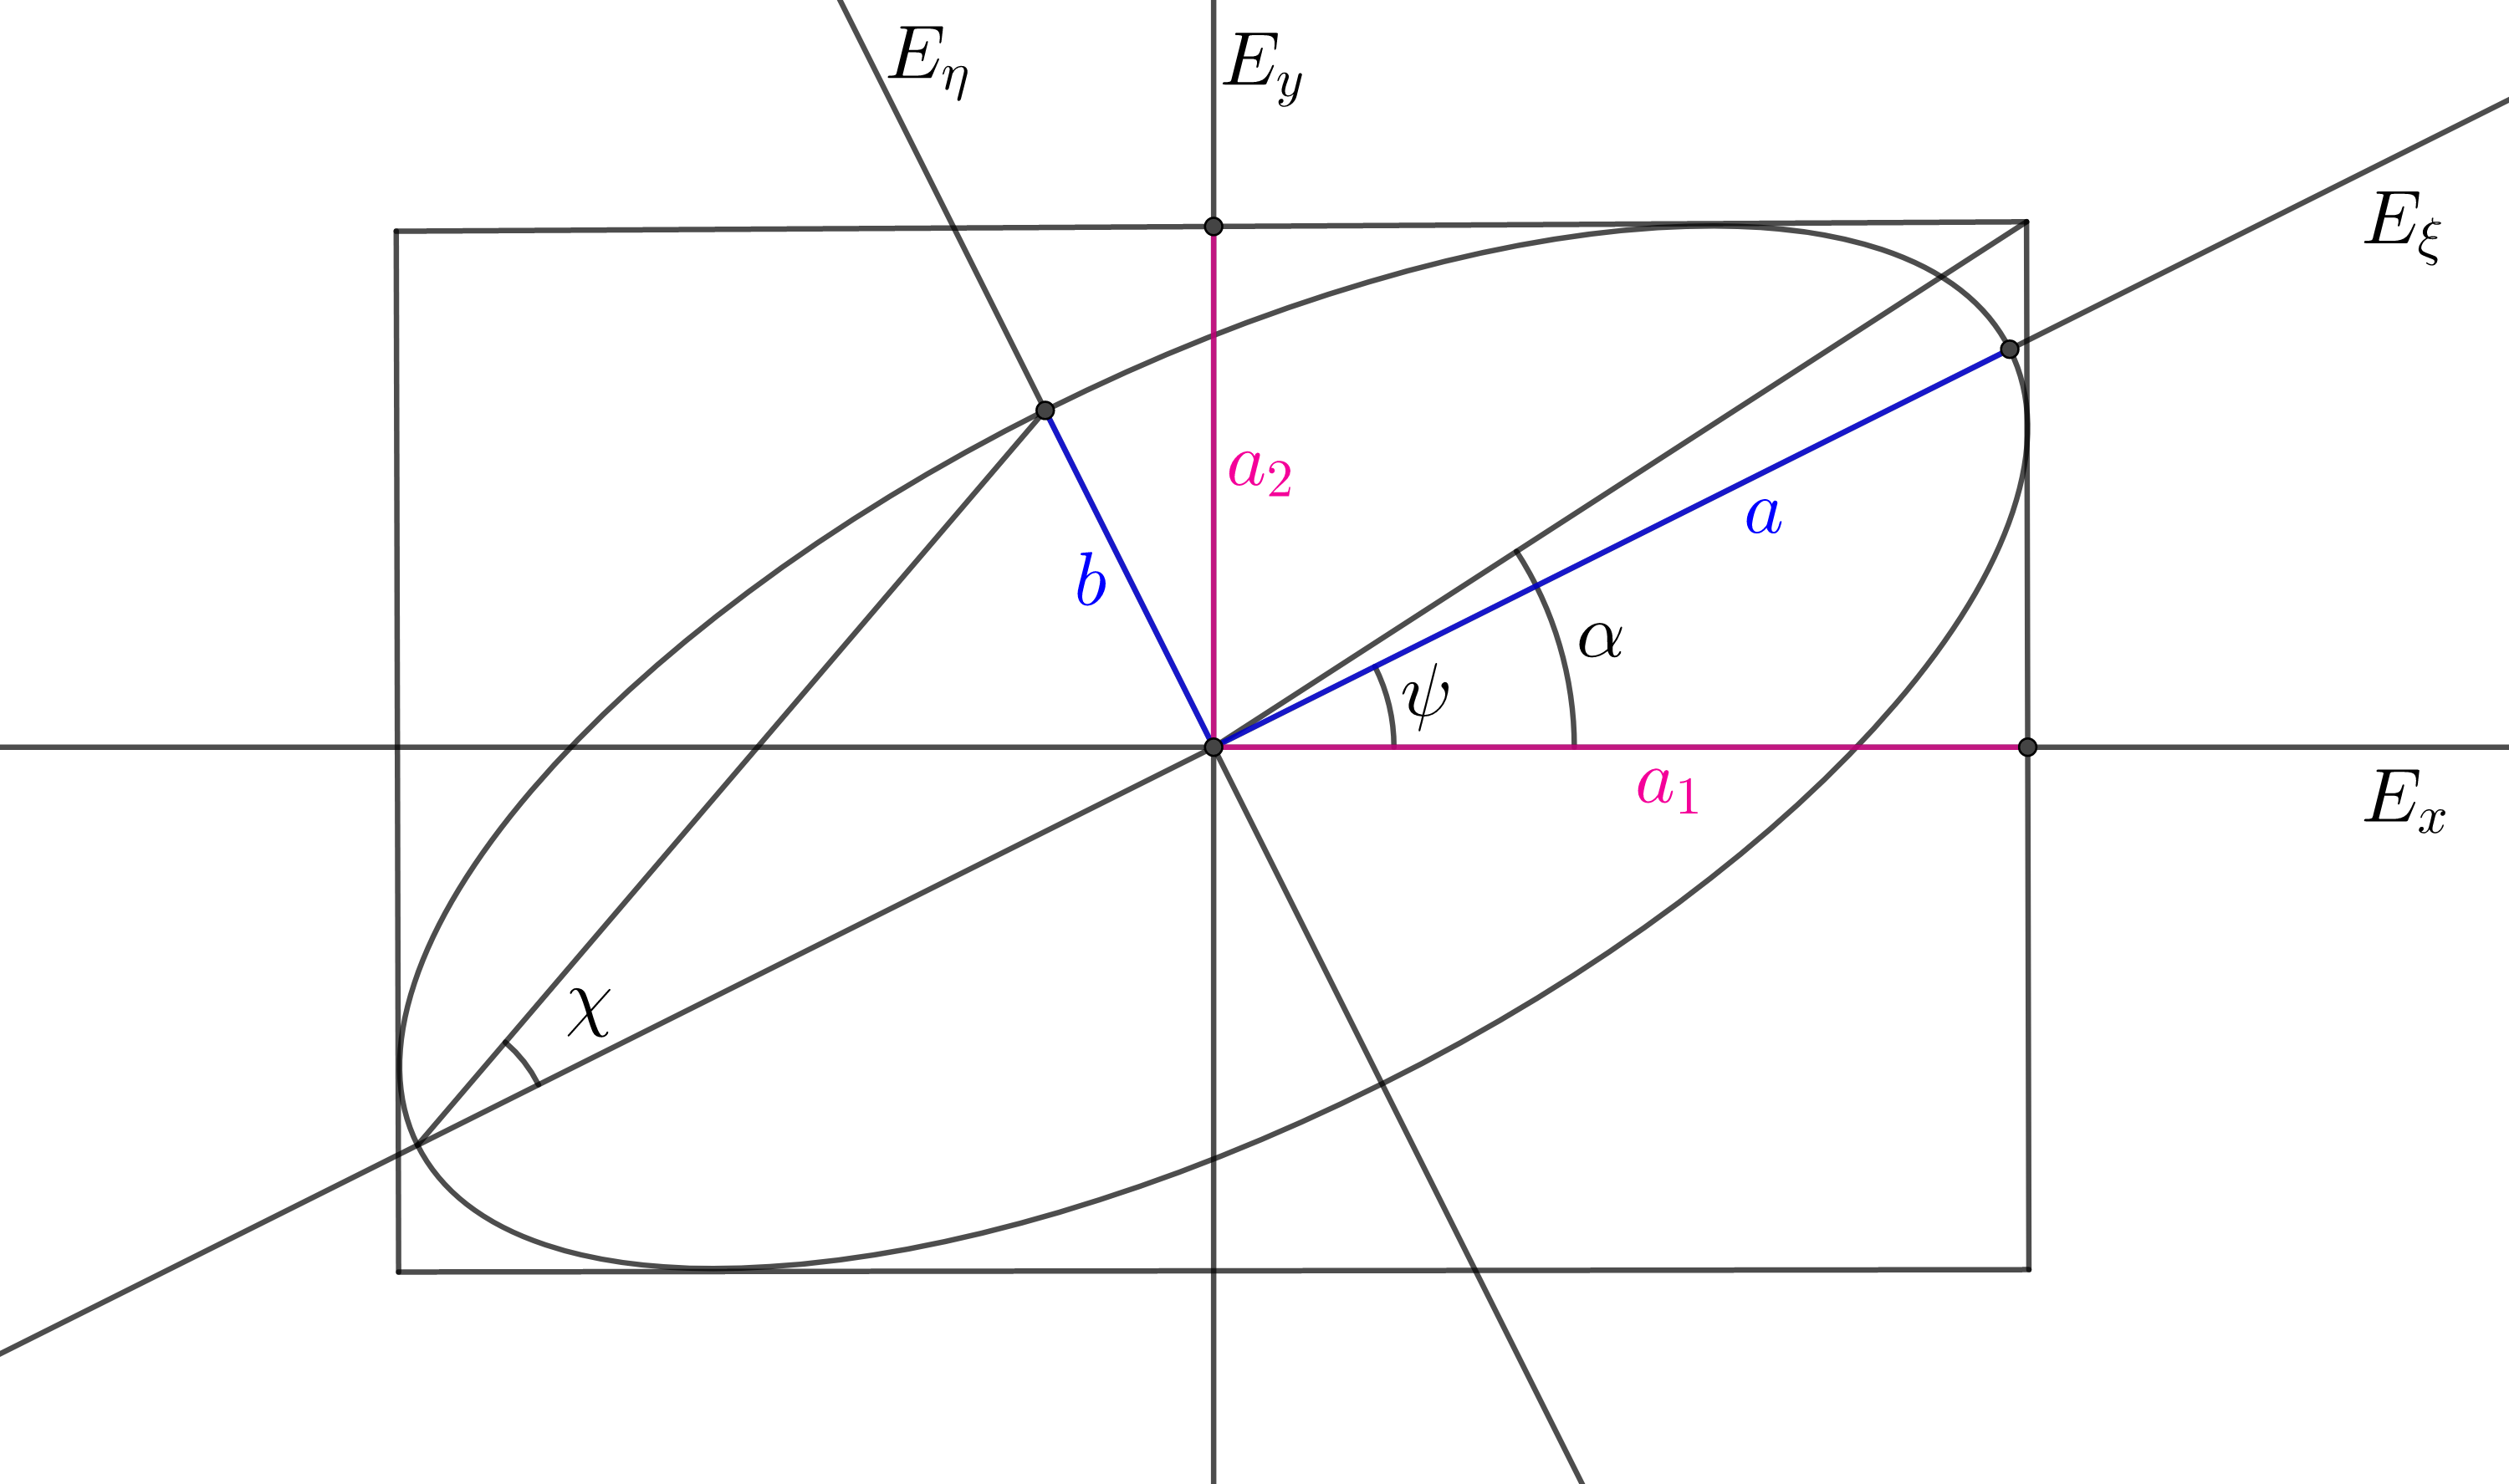
\includegraphics[width=8cm]{ellipse.png}
	\caption{Polarization ellipse}
	\label{fig:pol ellipse}
\end{figure}

Let $\psi$ be the azimuth angle of the ellipse then 
\begin{align}
	\boldsymbol{F}&= R(\psi)\:\boldsymbol{E}\\
	\Rightarrow\begin{bmatrix}E_\xi\\E_\eta\end{bmatrix}&= 
	\begin{bmatrix}
		\cos\psi & \sin\psi \\
		-\sin\psi & \cos\psi
	\end{bmatrix}
	\begin{bmatrix}E_x\\F_y\end{bmatrix}\\
	\Rightarrow
	\begin{bmatrix}
		a \cos(\tau+\delta_0)\\
		\pm b \sin(\tau+\delta_0)
	\end{bmatrix}&=
	\begin{bmatrix}
		\cos\psi & \sin\psi \\
		-\sin\psi & \cos\psi
	\end{bmatrix}
	\begin{bmatrix}
		a_1 \cos(\tau+\delta_1)\\
		a_2 \cos(\tau+\delta_2)
	\end{bmatrix}
\end{align}

We want value of $a, b$, After some tedious calculation \cite{born-wolf}, we reach to some important results, given below 
\begin{align}
	& a^2 + b^2 = a_1^2 + a_2^2\\
	&\pm ab = a_1a_2\sin\delta \label{eq:1.50}\\ 
	&\tan \chi \vcentcolon= \pm\frac{b}{a} \label{eq:1.51}\text{ where } \chi\in[-\frac{\pi}{4},\frac{\pi}{4}]\\
	&\tan \alpha \vcentcolon= \frac{a_2}{a_1} \text{ where } \alpha\in[0,\frac{\pi}{2}]\\
	&\tan 2\psi = \tan 2\alpha \cos\delta\\
	&\sin 2\chi = \sin 2\alpha \sin\delta
\end{align}
where $\psi$ is the \textit{azimuth} and $\chi$ is \textit{ellipticity} of the polarization ellipse. 

To see the handedness of the rotation of electric field vector in transverse plane,
\begin{enumerate}
	\item[\textbf{Case I}] 
	For right-handed polarization, $\sin\delta>0$, then from equations \ref{eq:1.50}, and \ref{eq:1.51}, we can say 
	$$\tan \chi \ge 0\Rightarrow \chi \in \left(0,\frac{\pi}{4}\right]$$
	
	\item[\textbf{Case II}] 
	Similarly for left-handed polarization, $\sin\delta<0$, then from equations \ref{eq:1.50}, and \ref{eq:1.51}, we can say 
	$$\tan \chi \le 0\Rightarrow \chi \in \left[-\frac{\pi}{4},0\right)$$
\end{enumerate}
	
Now the Jones vector of elliptical polarization in the form of ellipticity and azimuth will be, \cite{WO}
\begin{align}
	\boldsymbol{J}= 
		\begin{bmatrix}
			\cos\psi\cos\chi- i \sin\psi\sin\chi \\
			\sin\psi\cos\chi+ i \cos\psi\sin\chi
		\end{bmatrix}
\end{align}

\subsubsection{Stokes vector and corresponding Poincare representation}
From the eq. \ref{eq:1.16}, we can write for our case, 
\begin{align}
	\boldsymbol{S}= \begin{bmatrix} S_0\\ S_1\\ S_2\\S_3\end{bmatrix} =
	\begin{bmatrix}
		{a_1^2 + a_2^2}\\
		{a_1^2 - a_2^2}\\
		{2a_1a_2\cos\delta}\\
		{2a_1a_2\sin\delta}
	\end{bmatrix}=S_0
	\begin{bmatrix}
		1\\
		\cos 2\chi \cos 2\psi\\
		\cos 2\chi \sin 2\psi\\
		\sin 2\chi
	\end{bmatrix}
\end{align}

So in Poincare sphere representation with axes $\{S_1, S_2, S_3\}$, the required vector is
\begin{align}
	S_0
	\begin{bmatrix}
		1\\
		\cos 2\chi \cos 2\psi\\
		\cos 2\chi \sin 2\psi\\
		\sin 2\chi
	\end{bmatrix}\longrightarrow
	(S_0\cos 2\chi \cos 2\psi, S_0\cos 2\chi \sin 2\psi, S_0\sin 2\chi)
\end{align}

The evolution of azimuth ($\psi$) and ellipticity ($\chi$) of the polarization state in Poincare representation is shown in the figure \ref{fig:compare poincare}.

\begin{figure}[H]
	\begin{subfigure}[H]{0.48\textwidth}
		\centering
		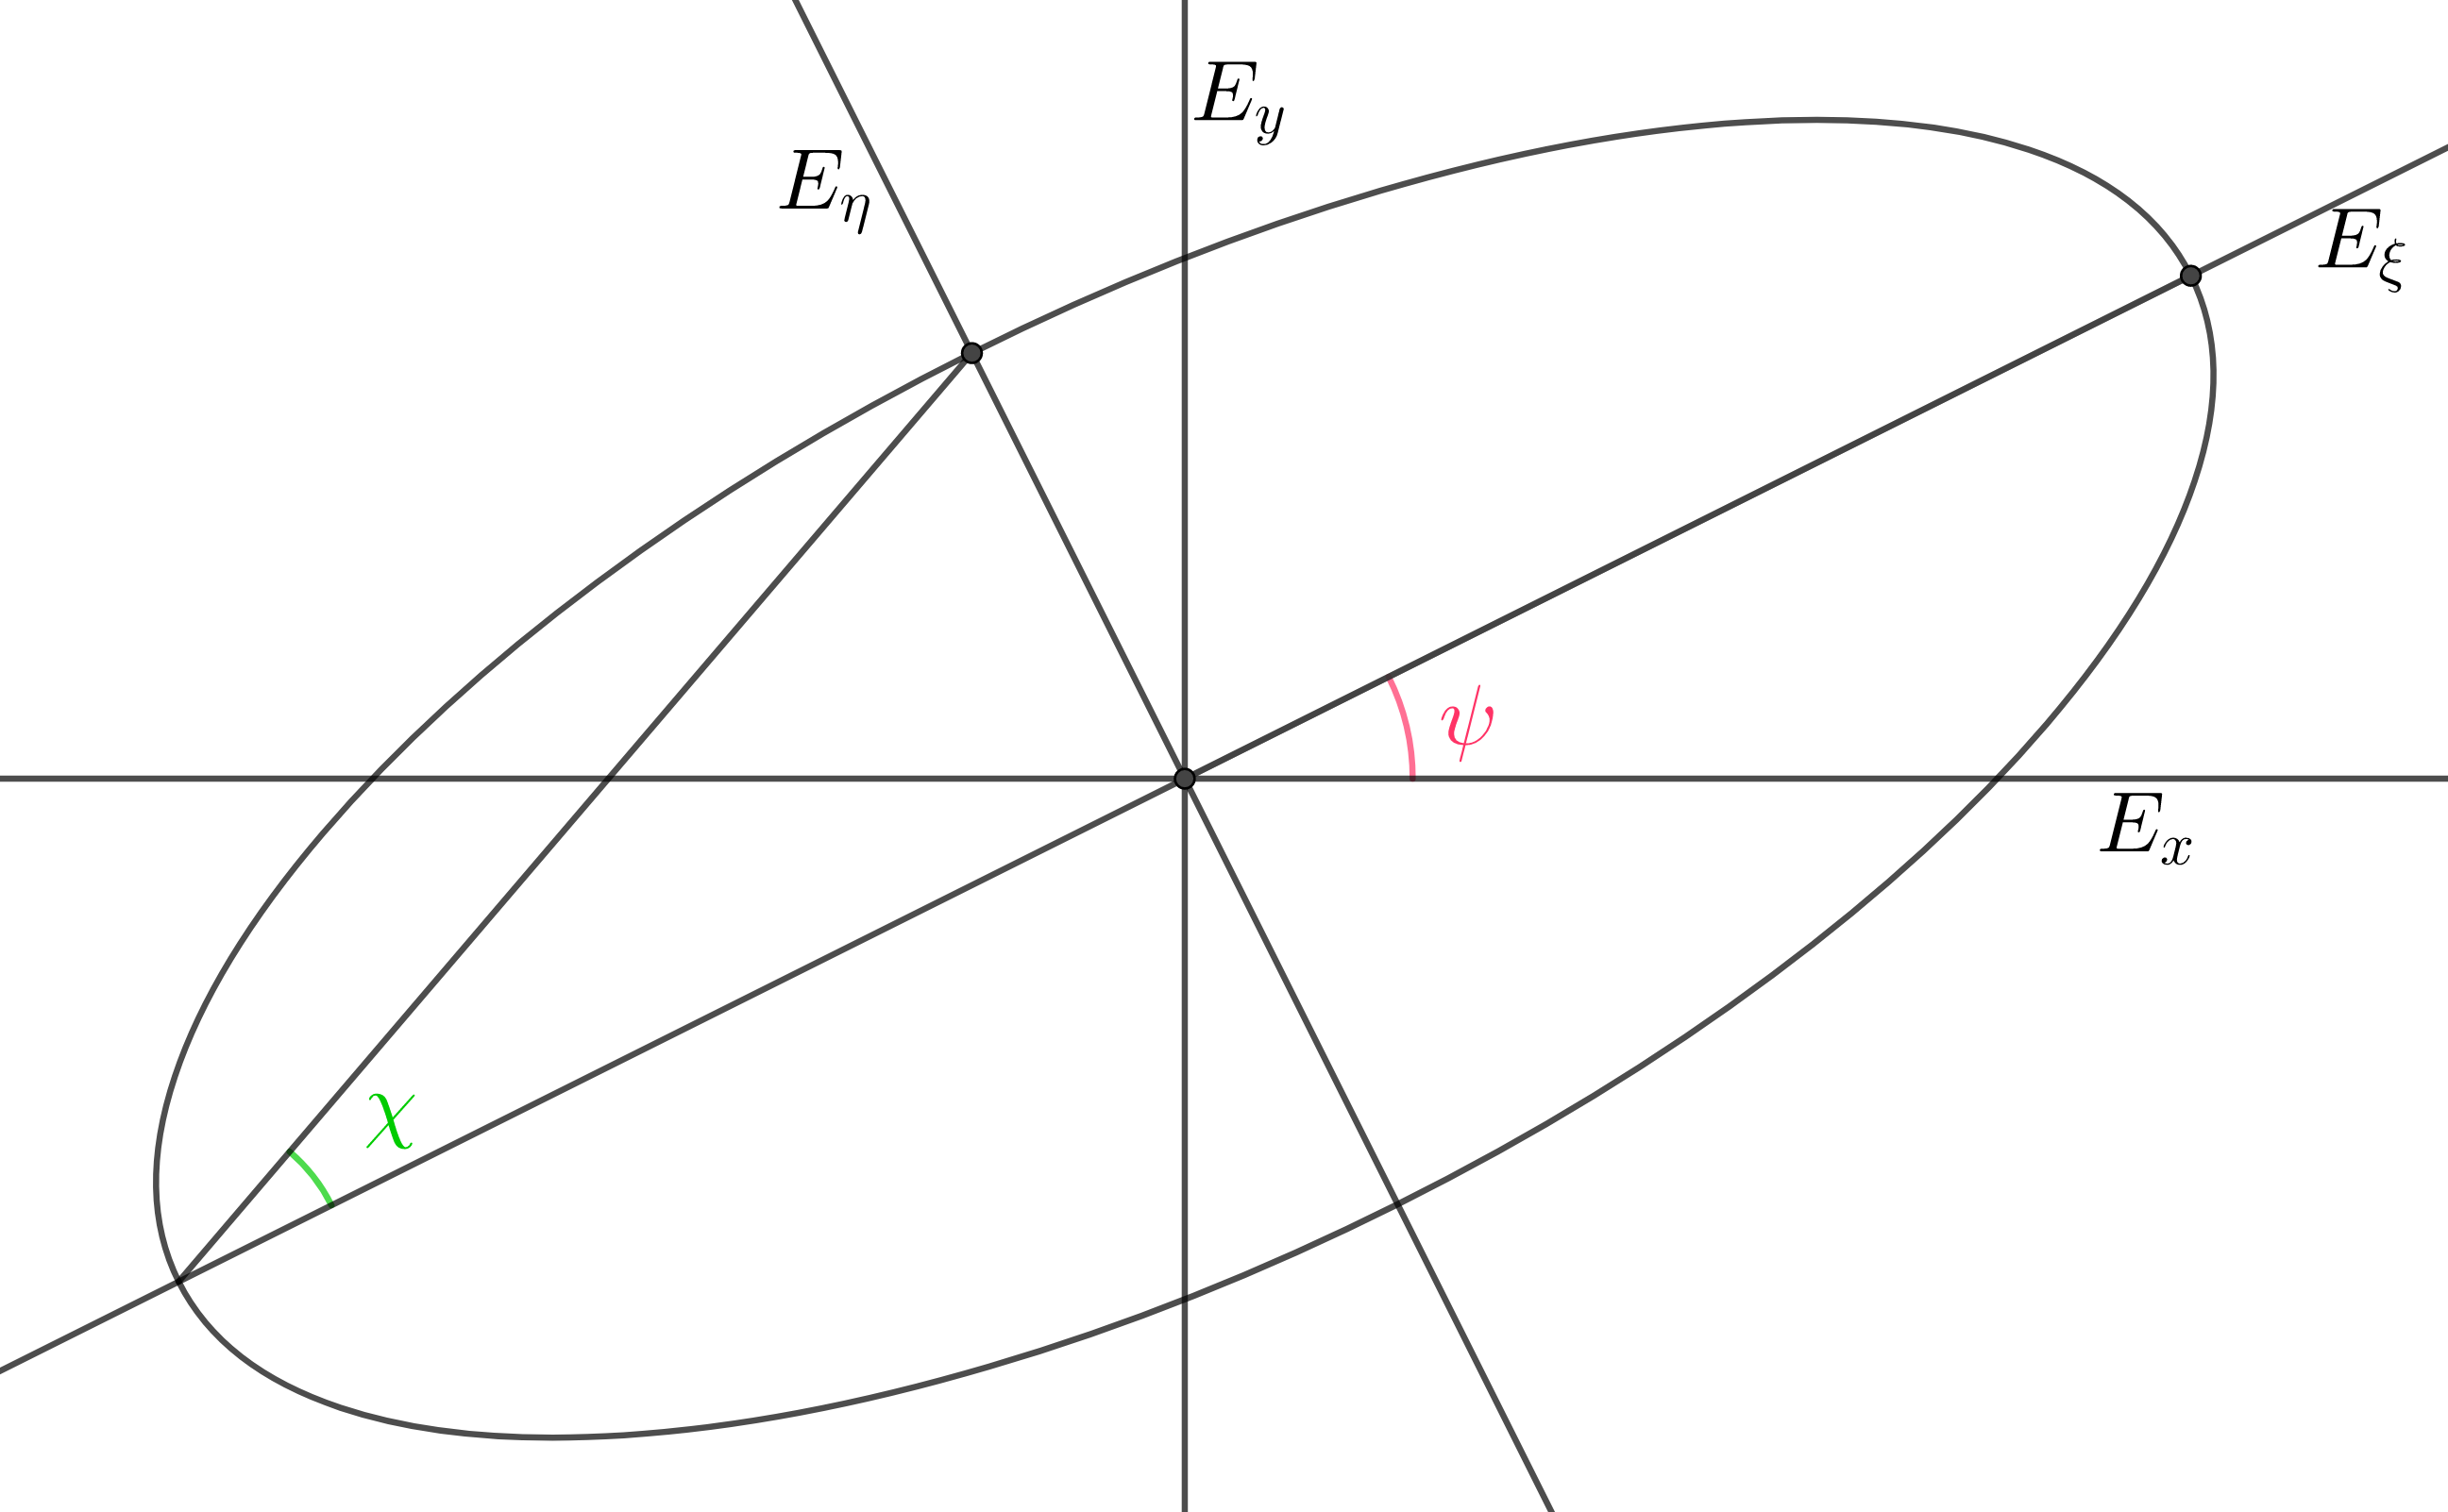
\includegraphics[width=0.9\textwidth]{ellipse_new}
		\caption{}
	\end{subfigure}
	\hfill
	\begin{subfigure}[H]{0.48\textwidth}
		\centering
		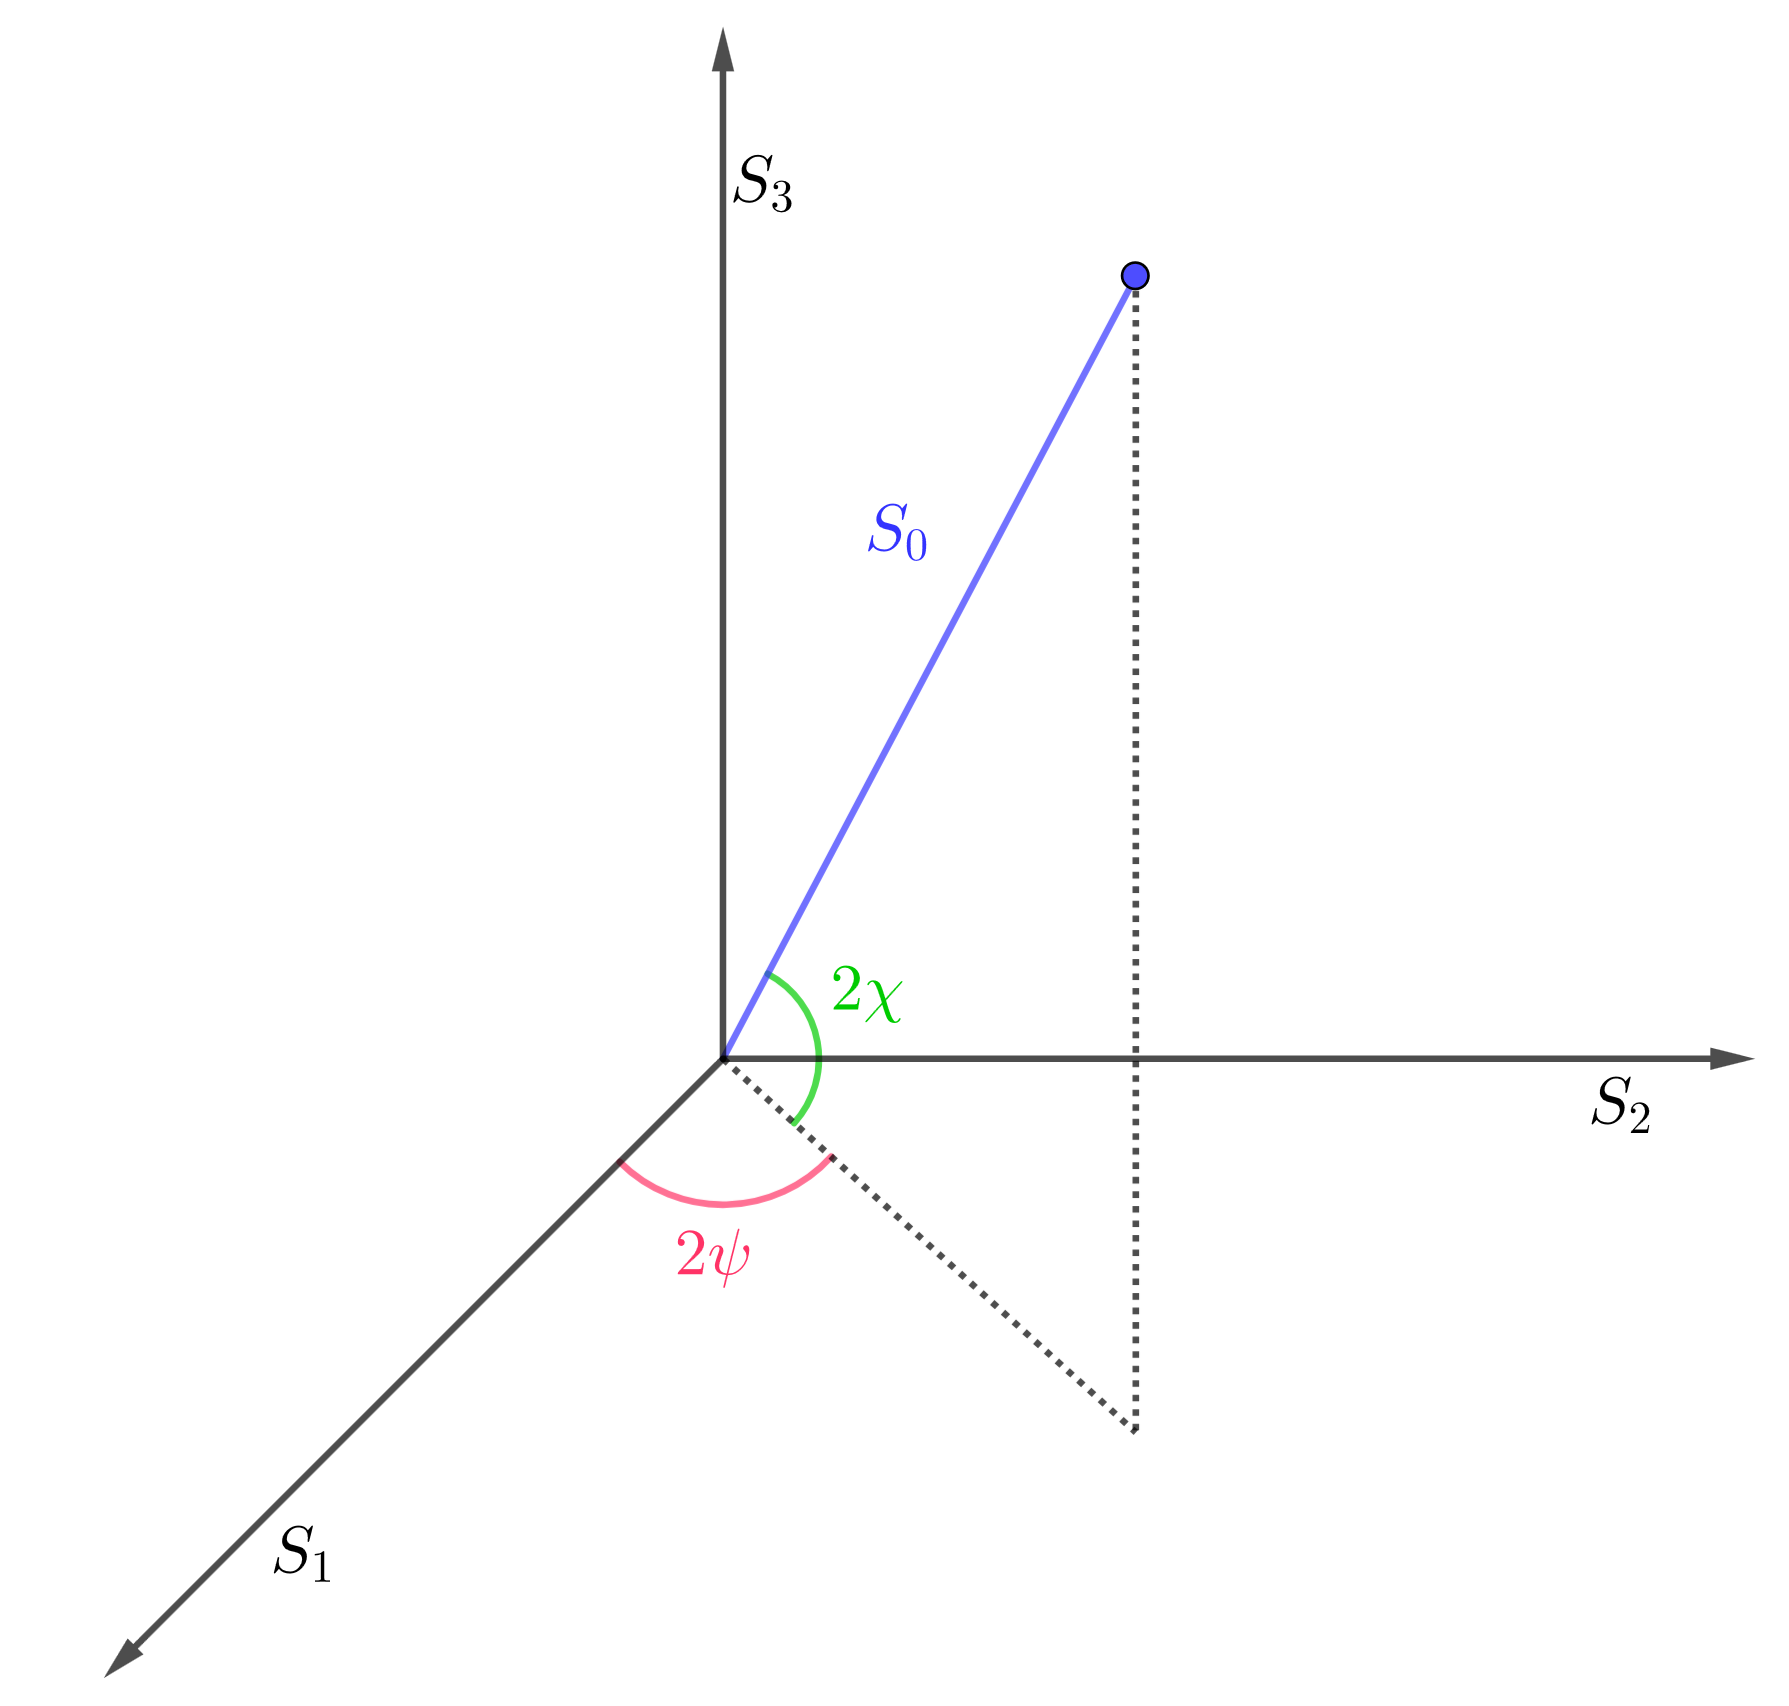
\includegraphics[width=0.7\textwidth]{poincare}
		\caption{}
	\end{subfigure}
	\caption{polarization ellipse and corresponding Poincare representation}
	\label{fig:compare poincare}
\end{figure}
For any $\psi$ and $\chi$ in the domain, the locus of state of polarization in Poincare sphere representation will always be on the sphere about origin of radius $S_0$. The pole and equatorial positions denotes the circular and linear polarization, respectively.
\clearpage



%%%%%%%%%%%%%%%%%%%%%%%%%%%%%%%%%%%%%%%%%%%
\section{GAUSSIAN BEAM}
\subsection{Introduction}
In optics and laser physics, the Gaussian beam stands as a fundamental concept, where the intensity of the light beam follows Gaussian curve. Its elegance lies in the fact that, it propagate over long distances with minimal divergence and diffraction. This distinctive feature makes it a preferred choice in a wide array of applications in optics and laser physics. Here we will briefly discuss about the different modes of Gaussian beams, as well as their properties.

\subsection{Paraxial wave equation}
From Maxwell's 3-D wave equation for electric field in vacuum,
\begin{align}
	\nabla^2\boldsymbol{E}(\boldsymbol{r},t) - \frac{1}{c^2}\frac{\partial^2}{\partial t^2}\boldsymbol{E}(\boldsymbol{r},t)=0 \label{eq:2.1}
\end{align}
Here we will consider the scalar form of the equation.

To find the scalar solution, let our first ansatz be,
\begin{align}
	{E}(x,y,z,t)= {F}(x,y,z) e^{i\omega t} \label{eq:2.2}
\end{align}
Putting it in eq. \ref{eq:2.1}, we get time -independent \textit{Helmholtz equation} \textit{i.e.} 
\begin{align}
	\nabla^2{F}(x,y,z) + k^2{F}(x,y,z)=0
	\text{ where }k^2 = \frac{\omega^2}{c^2} \label{eq:2.3}
\end{align}
For light to travel in z-direction, our 2nd ansatz be,
\begin{align}
	{F}(\boldsymbol{r}) = \psi(x,y,z)e^{-ikz}  \label{eq:2.4} 
\end{align}
Considering the slowly varying envelope approximation\cite{WO} that,
\begin{align}
	\left|\frac{\partial^2\psi}{\partial z^2}\right|\ll
	k \left|\frac{\partial\psi}{\partial z}\right| \ll
	k^2\left|\psi\right| \label{eq:2.5}
\end{align}
and putting \ref{eq:2.4} in eq. \ref{eq:2.3} gives \textit{Paraxial wave equation},
\begin{align}
	\nabla_T ^2\psi -2ik \frac{\partial\psi}{\partial r}=0 \label{eq:2.6}
\end{align}
where transverse Laplacian, $\displaystyle\nabla_T = \frac{\partial^2}{\partial x^2}+\frac{\partial^2}{\partial y^2}$ or in cylindrical coordinate, $\displaystyle\nabla_T = \frac{1}{r}\frac{\partial}{\partial r}\left(r\frac{\partial}{\partial r}\right) + \frac{1}{r^2}\frac{\partial^2}{\partial \phi^2}$.

\subsection{Scalar wave solution - Gaussian beam}
We will solve the paraxial wave equation in cylindrical coordinate $\{r,\phi,z \}$. \cite{cornell}
To get a solution for which intensity is of Gaussian like and radially symmetric (\textit{i.e.} no variation with $\phi$), our first ansatz be, \cite{kogelnik 66}\cite{cornell}
\begin{align}
	\psi(\boldsymbol{r},z)= A \exp\left[-i\left(p(z) + \frac{kr^2}{2q(z)}\right)\right]
	=A\:\underbrace{\exp\left[-ip(z)\right]}_{\text{first term}} \:\underbrace{\exp\left[-i\frac{kr^2}{2q(z)}\right]} _{\text{second term}} \label{eq:2.7}
\end{align} 
where second term is related to Gaussian intensity and first term is additional phase factor. Putting this, in eq, \ref{eq:2.6}, we get
\begin{align}
	\left[\frac{k^2}{q^2}\left(\frac{dq}{dz}-1\right)r^2 -2k\left(\frac{dp}{dz}+\frac{i}{q}\right)\right]\psi= 0
\end{align}
To satisfy this, for all $r$, we get
\begin{align}
	\frac{dq}{dz}-1 &=0 \label{eq:2.9}\\
	\frac{dp}{dz}+\frac{i}{q} &=0\label{eq:2.10}
\end{align}

Lets first calculate eq. \ref{eq:2.9}.
\begin{align}
	\frac{dq}{dz}-1 =0 
	\Rightarrow q(z) = z + q_0 \label{eq:2.11}
\end{align}
putting this in the second term of expression \ref{eq:2.7} at $z=0$,
\begin{align}
	\exp\left[-i\frac{kr^2}{2q(0)}\right] = \exp\left[-i\frac{kr^2}{2q_0}\right]
\end{align}
which is a phase factor does not give Gaussian intensity. So to get Gaussian intensity, $q_0$ must be imaginary. Let $q_0=iz_0$, then 
\begin{align}
	\boxed{q(z) = z + iz_0} \label{eq:2.13}
\end{align}

Now, the second term of expression \ref{eq:2.7} at $z=0$ be,
\begin{align}
	\exp\left[-\frac{kr^2}{2z_0}\right] = \exp\left[-\frac{r^2}{w_0^2}\right]
\end{align}
where
\begin{align}
	w_0^2=\frac{2z_0}{k}=\frac{\lambda z_0}{\pi}
	\Rightarrow \boxed{z_0 = \frac{\pi w_0^2}{\lambda} }
\end{align}
We call $z_0$ \textit{confocal parameter} or \textit{Rayleigh range} of the beam.

Now from expression \ref{eq:2.13}, we calculate $1/q(z)$.
\begin{align}
	\frac{1}{q(z)} = \frac{1}{z + iz_0} = \frac{z}{z^2 + z_0^2} - i\:\frac{z_0}{z^2 + z_0^2} \label{eq:2.16}
\end{align}
Then the second term of expression \ref{eq:2.7} be,
\begin{align}
	\exp\left[-i\frac{kr^2}{2q(z)}\right] = 
	\underbrace{\exp\left[-\frac{kr^2z_0}{2(z^2 + z_0^2)}\right]}_{\text{term A}}
	\underbrace{\exp\left[-i\frac{kr^2z}{2(z^2 + z_0^2)}\right]}_{\text{term B}} 
	\label{eq:2.17}
\end{align}

Write term A of \ref{eq:2.17} as 
\begin{align}
	\exp\left[-\frac{kr^2z_0}{2(z^2 + z_0^2)}\right] = \exp\left[-\frac{r^2}{w^2(z)}\right]
\end{align}
which is Gaussian, where
\begin{align}
	\boxed{w^2(z)= w_0^2\left[1+\left(\frac{z}{z_0}\right)^2\right]} \label{eq:2.19}
\end{align}
We call $w(z)$ \textit{physical radius/half-width} of the beam.

Write term B of \ref{eq:2.17} as 
\begin{align}
	\exp\left[-i\frac{kr^2z}{2(z^2 + z_0^2)}\right] = \exp\left[-i\frac{kr^2}{2 R(z)}\right]
\end{align}
where
\begin{align}
	\boxed{R(z)= z\left[1+\left(\frac{z_0}{z}\right)^2\right]} \label{eq:2.21}
\end{align}

We know for spherical wave,
\begin{align}
	{E}(\boldsymbol{r},t) \sim \frac{1}{r} e^{i(\omega t -kr)} \label{eq:2.22}
\end{align}

\begin{figure}[H]
	\centering
	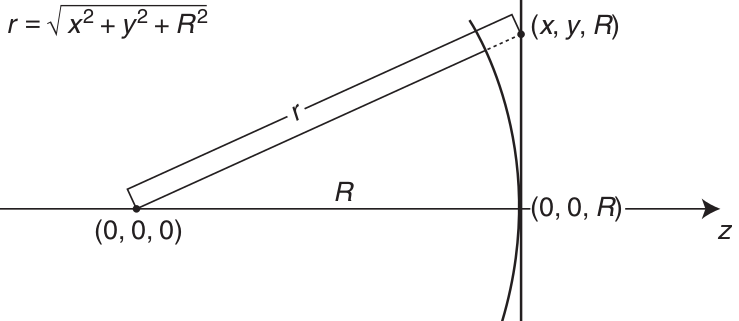
\includegraphics[width=7cm]{spherical wave.png}
	\caption{Radius of curvature of spherical wavefront (Ref. \cite{milonni})}
	\label{fig:sp wave}
\end{figure}
Let $R$ be the radius of curvature of spherical wavefront. 
Now for any point $\boldsymbol{r}=(x,y,R)$ on $z=R$ plane, $r$ will be
\begin{align}
	r=\sqrt{x^2+y^2+R^2}
\end{align}
For collimated beam, we restrict radius of curvature measurement near $\boldsymbol{r}=(0,0,R)$, so
\begin{align}
	r=\sqrt{x^2+y^2+R^2}\approx R + \frac{x^2+y^2}{2R}
\end{align}

Now from \ref{eq:2.22},
\begin{align}
	E(\boldsymbol{r},t) &\sim \frac{1}{r} e^{i\omega t} e^{-ikr} {e^{-ik\frac{x^2+y^2}{2R}}}
\end{align}
comparing with \ref{eq:2.2},
\begin{align}
	\psi({x,y,z}) &\sim e^{-ik\frac{x^2+y^2}{2R}} \label{eq:2.26}
\end{align}
comparing \ref{eq:2.26} in the above expression with term B of \ref{eq:2.17}, we conclude that $R(z)$ in \ref{eq:2.21} is \textit{radius of curvature} of wavefront near $r=0$ of collimated beam in far field.


Putting \ref{eq:2.19} and \ref{eq:2.21} in eq. \ref{eq:2.16},
\begin{align}
	\boxed{\frac{1}{q(z)} = \frac{1}{R(z)} - i\: \frac{\lambda}{\pi w^2(z)}} \label{eq:2.27}
\end{align}


Now we simplify the first term in \ref{eq:2.7}. Putting \ref{eq:2.13} in \ref{eq:2.10} and by solving the differential equation,  we get,
\begin{align}
	\frac{dp}{dz}= \frac{-i}{q} =\frac{-i}{z+iz_0} \Rightarrow i\:p(z) = \ln\left[1- i \frac{z}{z_0}\right]
\end{align}
As we can write
$$
1- i \frac{z}{z_0} = \sqrt{1+ \left(\frac{z}{z_0}\right)^2} \exp\left[{-i\:\tan[-1](\frac{z}{z_0})}\right]
$$
putting this in the above expression of $i\:p(z)$, our final expression will be
\begin{align}
	i\:p(z)=\frac{1}{2}\ln\left[1+ \left(\frac{z}{z_0}\right)^2\right]-i\: \tan[-1](\frac{z}{z_0}) \label{eq:2.29}
\end{align}

Finally putting \ref{eq:2.27} and \ref{eq:2.29} in \ref{eq:2.7}, we get, \cite{kogelnik 66}\cite{cornell}
\begin{align}
	\psi(\boldsymbol{r},z)&= A\exp\left[-i\left(p(z) + \frac{kr^2}{2q(z)}\right)\right]\nonumber\\
	&= A\exp\left[- \frac{1}{2}\ln\left[1+ \left(\frac{z}{z_0}\right)^2\right]+i\: \tan[-1](\frac{z}{z_0}) -i \frac{kr^2}{2}\left(\frac{1}{R(z)} - i\: \frac{\lambda}{\pi w^2(z)}\right) \right]\nonumber\\
	&=\frac{A}{\sqrt{1+ \left(\frac{z}{z_0}\right)^2}} \exp(i\:\tan[-1](\frac{z}{z_0})) \exp(-i\frac{kr^2}{2R(z)}) \exp(-\frac{r^2}{w^2(z)}) \nonumber\\
	\Rightarrow \psi(\boldsymbol{r},z)&=A\; 
	\underbrace{\left(\frac{w_0}{w(z)}\right)}_{\text{term I}}\;
	\underbrace{\exp(i{\:}\tan[-1](\frac{z}{z_0}))}_{\text{term II}}\; \underbrace{\exp(-i\frac{kr^2}{2R(z)})}_{\text{term III}}\;
	\underbrace{\exp(-\frac{r^2}{w^2(z)})}_{\text{term IV}} \label{eq:2.30}
\end{align} 
In that expression,
\begin{enumerate}
	\item Term I $\longrightarrow$ related to spreading of beam along propagation in z.
	\item Term II $\longrightarrow$ related to \textit{Gouy phase}.
	\item Term III $\longrightarrow$ gives radius of curvature of beam wave front.
	\item Term IV $\longrightarrow$ gives radially symmetric Gaussian intensity profile.
	
\end{enumerate}

\subsection{Characteristics of Gaussian Beam }
\begin{figure}[H]
	\centering
	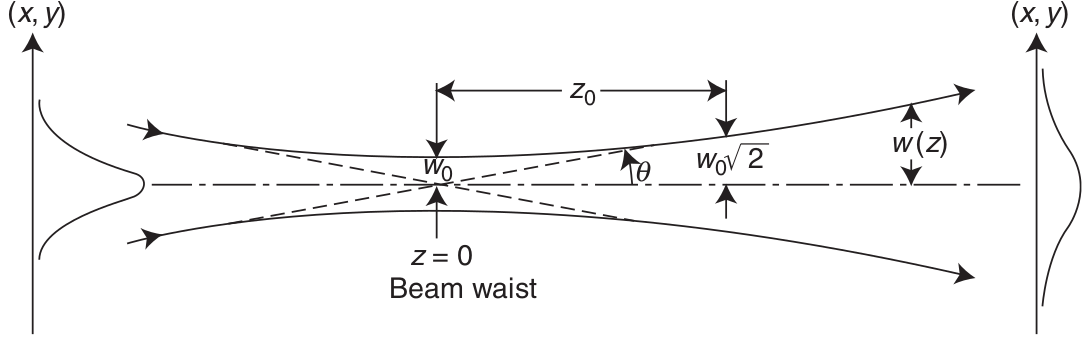
\includegraphics[width=0.7\textwidth]{beam.png}
	\caption{A beam profile (Ref. \cite{milonni})}
	\label{fig:beam}
\end{figure}

Some characteristics of Gaussian beam are
\begin{enumerate}
	\item 
	\textit{Intensity} of Gaussian beam in any transverse plain is, 
	\begin{align}
		I(r,z)&= \frac{1}{2}\epsilon_0c\abs{E^\ast E} = \frac{1}{2}\epsilon_0c\abs{\psi^\ast \psi}\nonumber\\
		&= \frac{1}{2} \epsilon_0c \abs{A}^2 \left(\frac{w_0}{w(z)}\right)^2  \exp(-\frac{2r^2}{w^2(z)})
	\end{align}
	\begin{figure}[H]
		\begin{subfigure}[H]{0.49\textwidth}
			\centering
			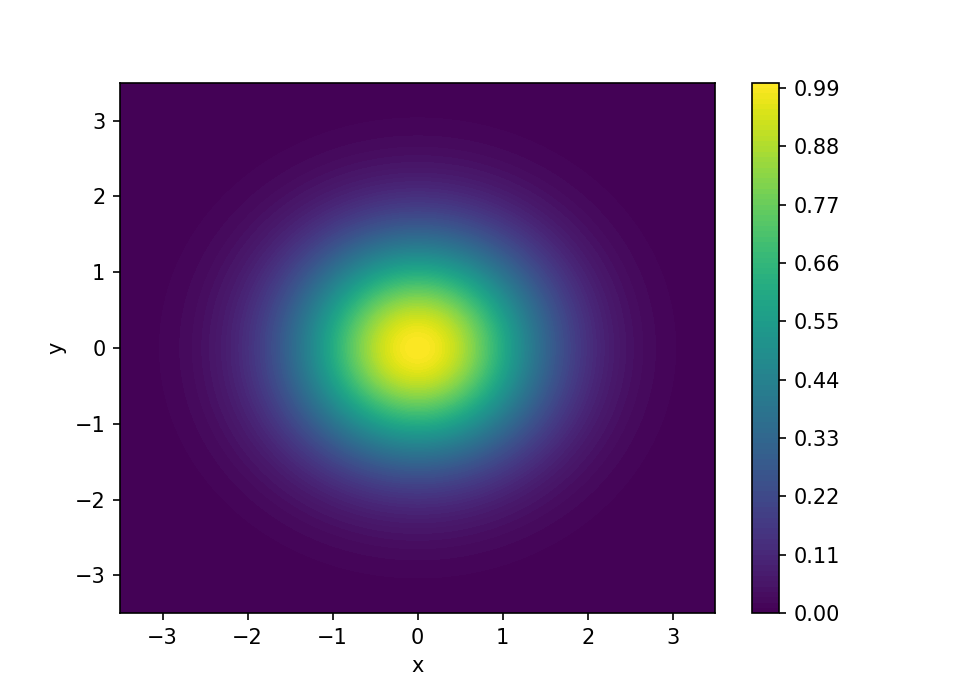
\includegraphics[width=0.9\textwidth]{intensity.png}
			\caption{Intensity variation in a cross section}
			\label{fig:g intensity}
		\end{subfigure}
		\hfill
		\begin{subfigure}[H]{0.49\textwidth}
			\centering
			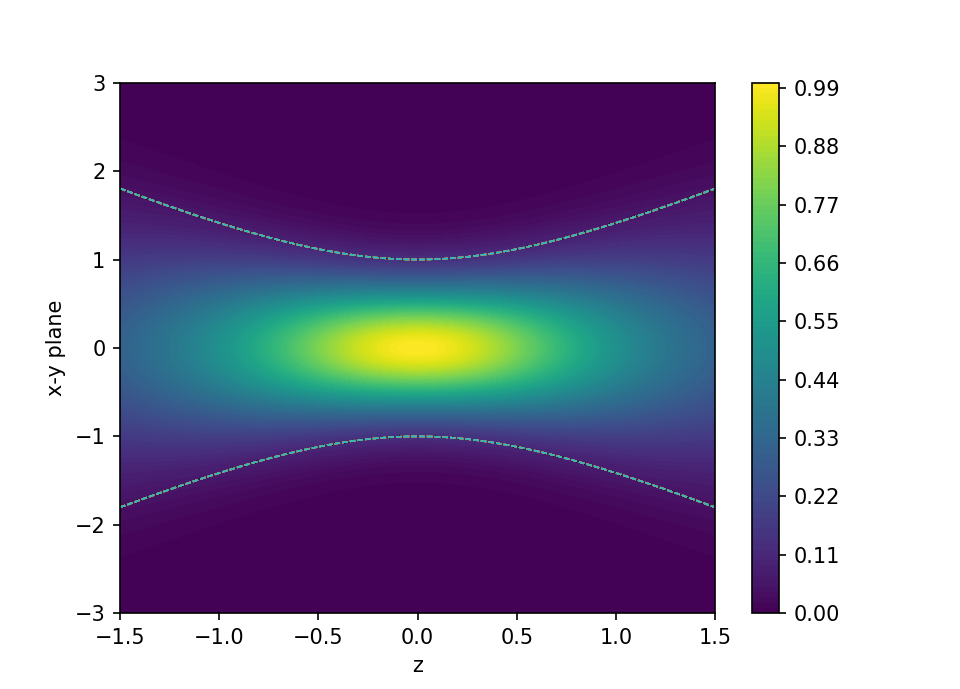
\includegraphics[width=0.9\textwidth]{intensity_var.png}
			\caption{Intensity variation along z-axis}
			\label{fig:g intensity var}
		\end{subfigure}
		\caption{Gaussian intensity profile for $z_0=1,w_0=1$}
	\end{figure}
	
	\item
	\textit{Rate of energy} of Gaussian beam passes through any transverse plain is given by
	\begin{align}
		W&= \iint_{-\infty}^{\infty} dx\:dy\:I(x,y,z)\nonumber\\
		&= \frac{1}{2} \epsilon_0c \abs{A}^2 \left(\frac{w_0}{w(z)}\right)^2 \iint_{-\infty}^{\infty} dx\:dy\: \exp(-\frac{2(x^2+y^2)}{w^2(z)}\nonumber)\\
		&= \frac{1}{2} \epsilon_0c \abs{A}^2 \left(\frac{w_0}{w(z)}\right)^2 \int_{-\infty}^{\infty} dx\: \exp(-\frac{2x^2}{w^2(z)})\: \int_{-\infty}^{\infty} dy\: \exp(-\frac{2y^2}{w^2(z)})\nonumber\\
		&=  \frac{1}{2}\epsilon_0c \abs{A}^2 \left(\frac{w_0}{w(z)}\right)^2 (\sqrt{\pi} w(z))^2 = \frac{1}{2}\epsilon_0c \abs{A}^2 w_0^2
	\end{align} which is constant throughout the propagation along z-axis.
	
	\item
	\textit{Radius of curvature} $R(z)$ of the wavefront is given by
	\begin{align}
		R(z)= z\left[1+\left(\frac{z_0}{z}\right)^2\right]
	\end{align}
	\subitem For $z=0$ $R\rightarrow\infty$
	\subitem For $z>>z_0$, then $R\approx z$
	
	\begin{figure}[H]
		\centering
		\scalebox{0.7}{% This file was created with tikzplotlib v0.10.1.
\begin{tikzpicture}

\begin{axis}[
axis on top,
tick pos=both,
xlabel=\textcolor{black}{\(\displaystyle z\)},
xmin=0, xmax=6,
xtick style={color=black},
ylabel=\textcolor{black}{\(\displaystyle R(z)\)},
ymin=-0.1, ymax=7,
ytick style={color=black}
]
\addplot [blue]
table {%
0.144144177436829 7.08164405822754
0.156156182289124 6.56000232696533
0.168168187141418 6.11459684371948
0.186186194419861 5.55715370178223
0.204204201698303 5.10126304626465
0.222222208976746 4.72222232818604
0.240240216255188 4.40274047851562
0.25825822353363 4.13035106658936
0.276276350021362 3.89584159851074
0.294294357299805 3.69225358963013
0.312312364578247 3.514235496521
0.330330371856689 3.35760307312012
0.348348379135132 3.21903800964355
0.366366386413574 3.09587454795837
0.384384393692017 2.98594689369202
0.408408403396606 2.85693788528442
0.432432413101196 2.7449324131012
0.456456422805786 2.64724588394165
0.480480432510376 2.56173038482666
0.504504442214966 2.48664736747742
0.528528451919556 2.42057394981384
0.552552580833435 2.36233520507812
0.576576590538025 2.31095147132874
0.600600600242615 2.26560068130493
0.624624609947205 2.22558617591858
0.648648619651794 2.19031524658203
0.672672748565674 2.15927982330322
0.696696758270264 2.13204145431519
0.720720767974854 2.10822081565857
0.744744777679443 2.087486743927
0.768768787384033 2.06955003738403
0.792792797088623 2.05415654182434
0.82282280921936 2.03815126419067
0.852852821350098 2.02538800239563
0.882882833480835 2.01553583145142
0.912912845611572 2.00830769538879
0.94294285774231 2.00345253944397
0.978978991508484 2.00045132637024
1.01501500606537 2.00022220611572
1.05105102062225 2.00247955322266
1.09309303760529 2.00792837142944
1.13513517379761 2.01608753204346
1.17717719078064 2.02666687965393
1.22522521018982 2.04140162467957
1.273273229599 2.05865073204041
1.32732737064362 2.08072090148926
1.38738739490509 2.10816669464111
1.44744741916656 2.13831877708435
1.51351356506348 2.17422771453857
1.58558559417725 2.21626734733582
1.66366362571716 2.26474666595459
1.74774777889252 2.31991267204285
1.83783781528473 2.38195538520813
1.93993997573853 2.45541977882385
2.04804801940918 2.53631782531738
2.16816806793213 2.62938690185547
2.30030035972595 2.73502612113953
2.44444441795349 2.85353541374207
2.60660672187805 2.99024724960327
2.78078079223633 3.14039206504822
2.97897887229919 3.31466436386108
3.19519519805908 3.50816512107849
3.44144153594971 3.73201727867126
3.71771764755249 3.9867000579834
4.02402400970459 4.27253150939941
4.37237215042114 4.60108137130737
4.76276254653931 4.97272491455078
5.2132134437561 5.40503358840942
5.73573589324951 5.91008138656616
6 6.16666650772095
};
\end{axis}

\end{tikzpicture}
}
		\caption{Variation of radius of curvature with z ($z_0=1$)}
		\label{fig:R vs z}
	\end{figure}
	
	\item
	\textit{Beam half-width} (see fig. \ref{fig:beam}) is given by 
	\begin{align}
		w(z)= w_0\sqrt{1+\left(\frac{z}{z_0}\right)^2}
	\end{align}
	\subitem For $z=0$, then $w = w_0$ (\textit{Beam waist})
	\subitem For $z>>z_0$, then $w(z)= w_0\frac{z}{z_0}$
	\subitem \textit{Diffraction angle} at far field is given by 
	\begin{align}
		2\theta = 2\lim_{z\to\infty}\frac{dw}{dz} = 2\frac{w_0}{z_0} = \frac{2\lambda}{\pi w_0}
	\end{align}
	\subitem \textit{Effective area} of the beam in a cross section is $\displaystyle \frac{1}{2} \pi w^2(z)$
	
	\item 
	\textit{Gouy phase} represents the difference in phase shift of a Gaussian beam \textit{w.r.t.} a plane wave of the same wavelength near $r=0$. \cite{conry 12}
	Gouy phase of a Gaussian beam is given by
	\begin{align}
		\phi_g (z) = \tan[-1](\frac{z}{z_0})
	\end{align}
	The Gouy phase vary form $-\pi/2$ to $\pi/2$ continuously as $z$ goes from $-\infty$ to $\infty$, shown in fig. \ref{fig:gouy}
	
	\begin{figure}[H]
		\centering
		\scalebox{0.7}{% This file was created with tikzplotlib v0.10.1.
\begin{tikzpicture}

\begin{axis}[
axis on top,
tick pos=both,
xlabel=\textcolor{black}{\(\displaystyle z/z_0\)},
xmin=-10, xmax=10,
xtick style={color=black},
ylabel=\textcolor{black}{\(\displaystyle \phi_g\)},
ymin=-1.5707963267949, ymax=1.5707963267949,
ytick style={color=black},
ytick={-1.5707963267949,-0.785398163397448,0,0.785398163397448,1.5707963267949},
yticklabels={
  \(\displaystyle -\pi/2\),
  \(\displaystyle -\pi/4\),
  0,
  \(\displaystyle \pi/4\),
  \(\displaystyle \pi/2\)
}
]
\addplot [blue]
table {%
-10 -1.47112762928009
-9.09909915924072 -1.46133458614349
-8.31831836700439 -1.45115387439728
-7.63763761520386 -1.44060635566711
-7.03703689575195 -1.42963624000549
-6.49649667739868 -1.41806590557098
-6.01601600646973 -1.40607941150665
-5.57557535171509 -1.39332950115204
-5.19519519805908 -1.38063657283783
-4.83483505249023 -1.36684000492096
-4.51451444625854 -1.3528083562851
-4.23423433303833 -1.33887565135956
-3.97397398948669 -1.32427728176117
-3.73373365402222 -1.30910956859589
-3.51351356506348 -1.2935129404068
-3.31331324577332 -1.27767729759216
-3.13313317298889 -1.26184701919556
-2.95295286178589 -1.24427378177643
-2.79279279708862 -1.22695517539978
-2.63263273239136 -1.20778226852417
-2.49249243736267 -1.18925178050995
-2.35235238075256 -1.16883552074432
-2.23223233222961 -1.14962184429169
-2.11211204528809 -1.12860548496246
-2.01201200485229 -1.10953962802887
-1.9119119644165 -1.08888971805573
-1.81181180477142 -1.06646966934204
-1.71171176433563 -1.04206764698029
-1.63163161277771 -1.02095758914948
-1.55155158042908 -0.998285889625549
-1.47147142887115 -0.973898887634277
-1.39139139652252 -0.94762659072876
-1.31131136417389 -0.919282674789429
-1.23123121261597 -0.888663530349731
-1.17117118835449 -0.864073634147644
-1.11111116409302 -0.837981224060059
-1.05105102062225 -0.810283184051514
-0.990990996360779 -0.78087329864502
-0.930930852890015 -0.749643564224243
-0.87087082862854 -0.716486573219299
-0.810810804367065 -0.68129825592041
-0.750750780105591 -0.643981456756592
-0.690690755844116 -0.604450702667236
-0.630630612373352 -0.5626380443573
-0.570570588111877 -0.518499135971069
-0.510510444641113 -0.472020626068115
-0.450450420379639 -0.42322850227356
-0.390390396118164 -0.372194886207581
-0.330330371856689 -0.319045424461365
-0.270270228385925 -0.26396369934082
-0.190190196037292 -0.187945485115051
-0.0900900363922119 -0.0898475646972656
0.190190196037292 0.187945485115051
0.270270228385925 0.26396369934082
0.330330371856689 0.319045424461365
0.390390396118164 0.372194886207581
0.450450420379639 0.42322850227356
0.510510444641113 0.472020626068115
0.570570588111877 0.518499135971069
0.630630612373352 0.5626380443573
0.690690755844116 0.604450702667236
0.750750780105591 0.643981456756592
0.810810804367065 0.68129825592041
0.87087082862854 0.716486573219299
0.930930852890015 0.749643564224243
0.990990996360779 0.78087329864502
1.05105102062225 0.810283184051514
1.11111116409302 0.837981224060059
1.17117118835449 0.864073634147644
1.23123121261597 0.888663530349731
1.31131136417389 0.919282674789429
1.39139139652252 0.94762659072876
1.47147142887115 0.973898887634277
1.55155158042908 0.998285889625549
1.63163161277771 1.02095758914948
1.71171176433563 1.04206764698029
1.81181180477142 1.06646966934204
1.9119119644165 1.08888971805573
2.01201200485229 1.10953962802887
2.11211204528809 1.12860548496246
2.23223233222961 1.14962184429169
2.35235238075256 1.16883552074432
2.49249243736267 1.18925178050995
2.63263273239136 1.20778226852417
2.77277278900146 1.22466564178467
2.93293285369873 1.24220144748688
3.11311316490173 1.25998544692993
3.29329323768616 1.27599668502808
3.49349355697632 1.29200482368469
3.71371364593506 1.30776298046112
3.95395398139954 1.32307946681976
4.21421432495117 1.33781325817108
4.49449443817139 1.35186803340912
4.79479455947876 1.3651841878891
5.13513517379761 1.37846660614014
5.49549531936646 1.39079856872559
5.89589595794678 1.40278565883636
6.35635614395142 1.41475248336792
6.85685682296753 1.42597782611847
7.41741752624512 1.43678653240204
8.05805778503418 1.44732820987701
8.77877902984619 1.45737421512604
9.59959983825684 1.46699965000153
10 1.47112762928009
};
\end{axis}

\end{tikzpicture}
}
		\caption{Variation of Gouy phase with z}
		\label{fig:gouy}
	\end{figure}
	
	\item 
	Inside Rayleigh length ($z_0$), the laser beam is highly collimated and intensity is also very high. So gain medium is kept in between $z=-z_0$ and $z_0$ to get maximum stimulated emission from gain medium.
\end{enumerate}


\subsection{Beam Tracing using ABCD matrix}
Like ray tracing using ABCD matrix, beam tracing is also done using ABCD matrix. We know that $q$ parameter gives all the characteristic of the beam as 
\begin{align*}
	q(z) &= z + iz_0\\
	\frac{1}{q(z)} &= \frac{1}{R(z)} - i\: \frac{\lambda}{\pi w^2(z)}
\end{align*}
\begin{figure}[H]
	\centering
	\includegraphics[width=0.5\linewidth]{"beam tracing"}
	\caption{Schematic of beam tracing}
	\label{fig:beam-tracing}
\end{figure}

By using ABCD matrix we can understand the change in $q$ parameter of input and output the Gaussian beam, say $q_{in}$ and $q_{out}$ respectively. Let the ABCD matrix of the optical element is 
\begin{align}
	\begin{bmatrix}
		A&B\\
		C&D
	\end{bmatrix}
\end{align}
Then relation between $q_{in}$ and $q_{out}$ is
\begin{align}
	q_{out}= \frac{Aq_{in}+B}{Cq_{in}+D}
\end{align}

\subsection{Resonator stability and resonator mode-frequency}
Now we will discuss about the \textit{resonator stability} for the Gaussian beam. The resonator cavity (or optical cavity) is made of two highly reflecting mirror align in particular manner so that  light confined in the cavity reflects multiple times, producing modes with certain resonance frequencies. \cite{opt cavity} If a Gaussian beam is to be a mode of a resonator with spherical mirrors, then radius of curvature of beam wave-front must be equal to that of the mirror.
\begin{figure}[H]
	\centering
	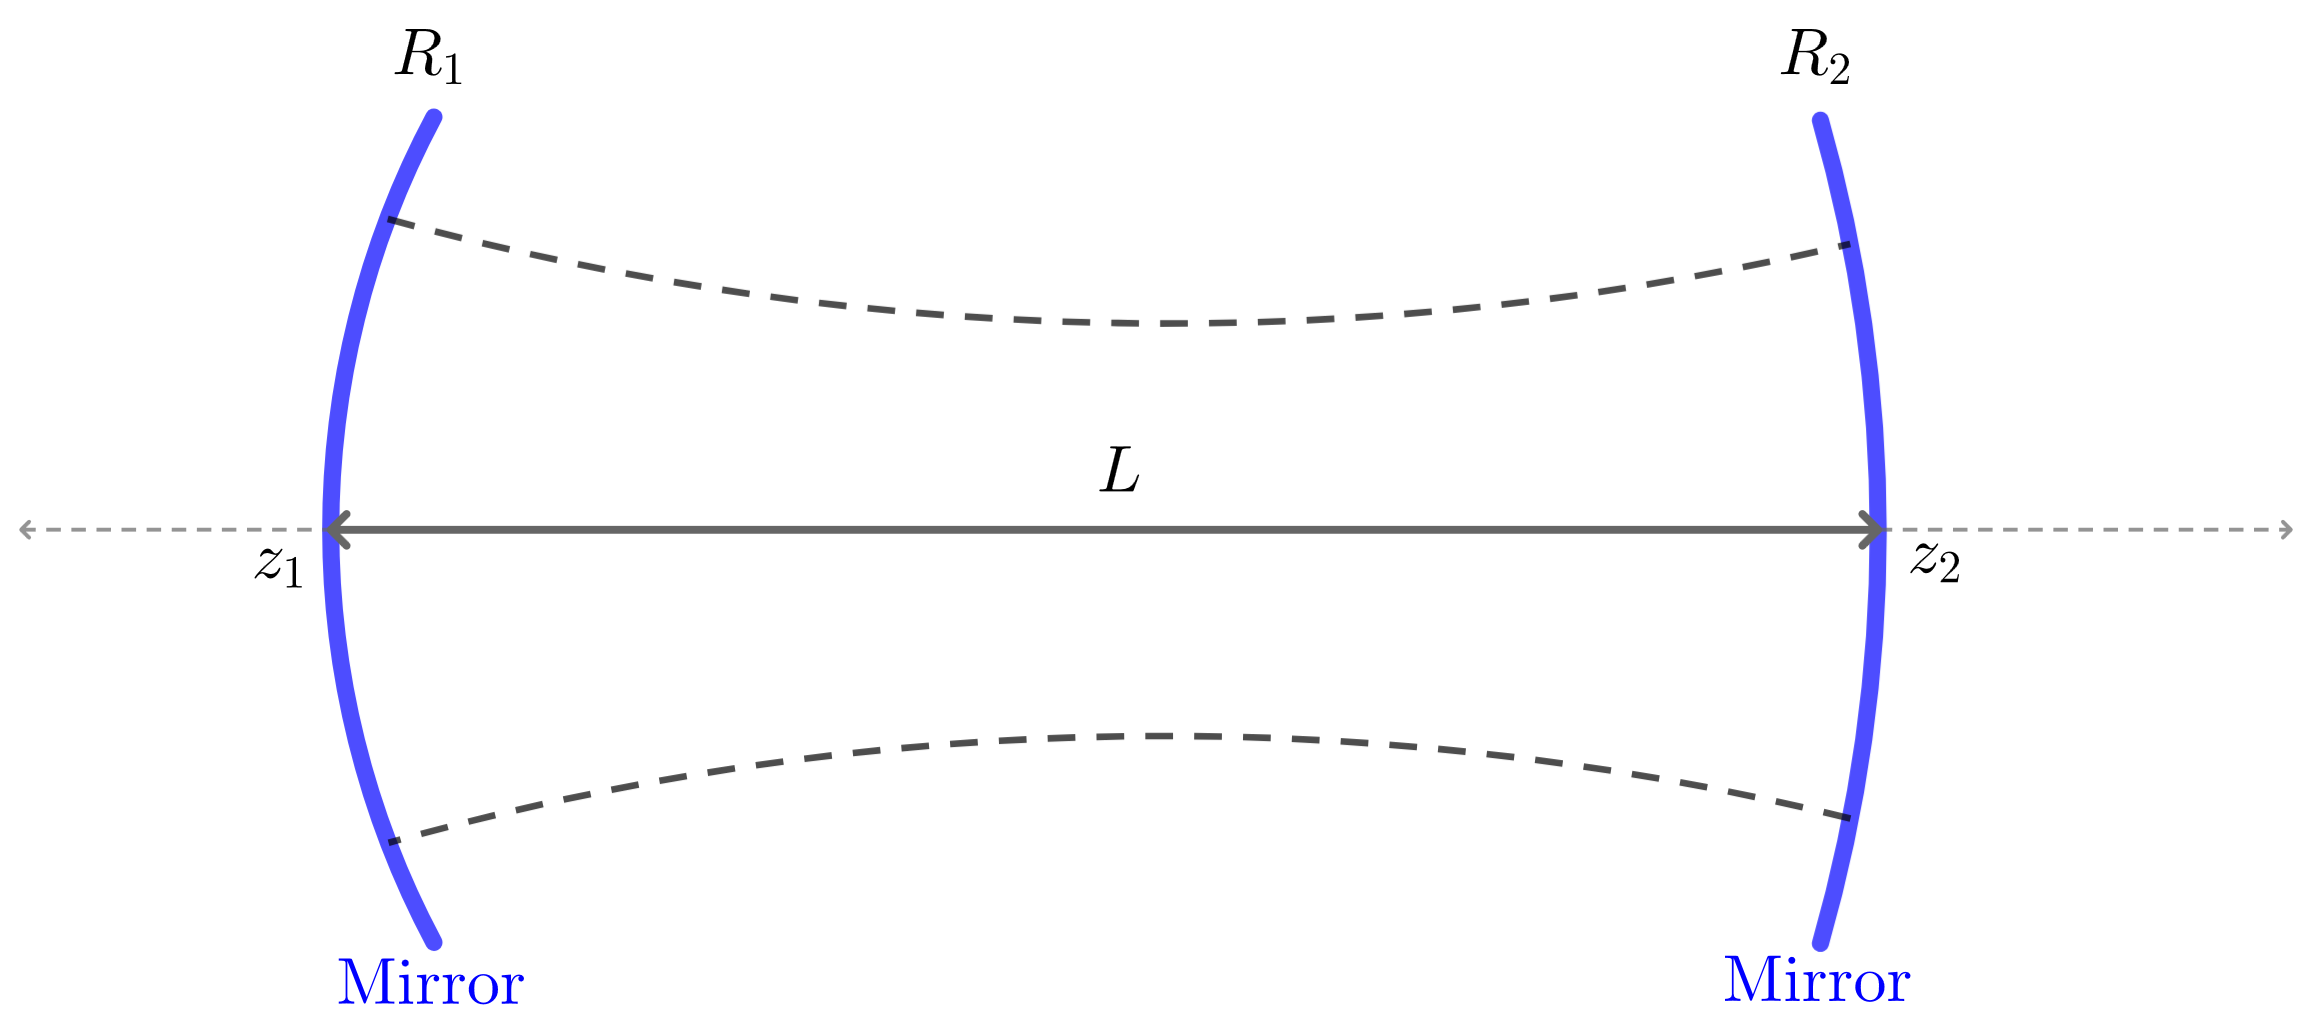
\includegraphics[width=0.6\linewidth]{resonator}
	\caption{Schematic of beam resonator of two mirrors of radius of curvature $R_1$ \& $R_2$}
	\label{fig:resonator}
\end{figure}

Let radius of curvature of first and second mirror are $R_1$ and $R_2$ respectively, length of resonator cavity is $L$, then \cite{milonni}
\begin{align}
	R(z_1)= z_1+\frac{z_0^2}{z_1}&=-R_1\\
	R(z_2)= z_2+\frac{z_0^2}{z_2}&= R_2\\
	z_2-z_1&=L
\end{align}

Lets define, 
\begin{align}
	g_i=1-\frac{L}{R_i}
\end{align}
where $R_i>0$ for concave and $<0$ for convex mirror. By considering the four relation, and the properties of Gaussian beam, we get, \cite{milonni}
\begin{enumerate}
	\item 
	Mirror locations \textit{w.r.t.} beam waist location, $z_0$ be
	\begin{align}
		z_1&=-\frac{Lg_2(1-g_1)}{g_1+g_2-2g_1g_2}\\
		z_2&=z_1+L
	\end{align}

	\item 
	Let spot sizes of beam at first, second mirrors and beam waist be $w_1$, $w_2$ and $w_0$ respectively, then
	\begin{align}
		w_1&= \left(\frac{\lambda L}{\pi}\right)^{1/2} \left(\frac{g_2}{g_1(1-g_1g_2)}\right)^{1/4}\\
		w_2&= \left(\frac{\lambda L}{\pi}\right)^{1/2} \left(\frac{g_1}{g_2(1-g_1g_2)}\right)^{1/4}\\
		w_0&= \left(\frac{\lambda L}{\pi}\right)^{1/2} \left(\frac{g_1g_2(1-g_1g_2)}{(g_1+g_2-2g_1g_2)^2}\right)^{1/4}
	\end{align}
\end{enumerate}

Note that $w_0$ to be a real value,
\begin{align}
	& g_1g_2(1-g_1g_2)>0\nonumber\\
	\Rightarrow& \boxed{g_1g_2 \notin [0,1]}
\end{align} This is the \textit{condition of stable resonator}. The cases when $g_1g_2= 0,1$ is neither stable nor unstable, is called \textit{marginal stability}.

From \ref{eq:2.4} and \ref{eq:2.30}, we see that the spatial phase of Gaussian beam near the centroid (\textit{i.e.} $r\approx0$) be
\begin{align}
	\Phi(z) = kz-\tan[-1](\frac{z}{z_0})
\end{align}
For light confined in the cavity to be in standing wave mode, phase change in a round trip \textit{i.e.} from first mirror after reflecting at second mirror to again first mirror, should be an integral multiple of $2\pi$. So phase change from first mirror to second mirror is an integral multiple of $\pi$. Then
\begin{align}
	\Phi(z_2)-\Phi(z_1) &= m\pi\nonumber\\
	k(z_2-z_1)- \left[\tan[-1](\frac{z_2}{z_0})-\tan[-1](\frac{z_1}{z_0})\right]&=m\pi \text{, where } m= 0, \pm1,\pm2 ,\dots
\end{align} 
If the mode frequency is $\nu$, $k=2\pi\nu/c$, then
\begin{align}
	\nu_m = \frac{c}{2L}\left[m+\frac{1}{\pi}\cos[-1](\sqrt{g_1g_2})\right]
\end{align} This is \textit{longitudinal mode} of Gaussian beam.

\subsection{Different modes of Gaussian beams}
Here we will discuss mainly two types of higher order Gaussian beams \textit{i.e.}
\begin{enumerate}
	\item Hermite-Gaussian (HG) beam
	\item Laguerre-Gaussian (LG) beam
\end{enumerate}

\subsubsection{Hermite-Gaussian beam}
In the expression \ref{eq:2.30}, we get the radially symmetric Gaussian beam solution. But we now seek higher order solution of Gaussian beam which is rectangular symmetric.

Lets take the ansatz as,
\begin{align}
	\psi(\boldsymbol{r},z)= A \: g\left(\frac{x}{w(z)}\right) h\left(\frac{y}{w(z)}\right) \exp\left[-i\left(p(z) + \frac{kr^2}{2q(z)}\right)\right]
\end{align}
Putting this in Paraxial wave equation \ref{eq:2.6}, and solving the differential equation, \cite{milonni} we get,
\begin{align}
	\psi_{m,n}(\boldsymbol{r},z)=& A \left(\frac{w_0}{w(z)}\right) H_m\left(\frac{\sqrt{2} x}{w(z)}\right) H_n\left(\frac{\sqrt{2} y}{w(z)}\right)\exp( -\frac{r^2}{w^2(z)}) \cdot\nonumber\\ 
	&\exp( i\:(m+n+1)\tan[-1](\frac{z}{z_0}) -i\frac{kr^2}{2R(z)}) \label{eq:2.53}
\end{align}
where $H_i$ is \textit{i th degree Hermite polynomial} and other symbols are as usual.
See for $m=0=n$ we recover the Gaussian solution of \ref{eq:2.30} which we call as \textit{zero order} HG beam. For different values of $m$ an $n$, we will get diferent type of higher order HG beam, these are called \textit{transverse electromagnetic mode} of order $(m,n)$ or, $TEM_{mn}$. 

Some characteristics of HG beams are given below,
	\begin{figure}[t]
	\foreach \n in {0,1,2}{
		\foreach \m in {0,1,2}{
			{
				\begin{subfigure}[htbp]{0.3\textwidth}
					\centering
					\includegraphics[width=\textwidth]{intensity_hg\n\m}
					\caption{$TEM_{\n\m}$}
					%\label{fig:hg\n\m}
				\end{subfigure}
				\hfill
			}
		}
	}
	\\
	\caption{Intensity variation for different TEM in a cross section ($z=0,z_0=1,w_0=1$)}
	\label{fig:hgmn}
\end{figure}
\begin{enumerate}
	\item 
	\textit{Intensity} of HG beam is given by
	\begin{align}
		I_{m,n}(x,y,z)=\frac{c\epsilon}{2} |A|^2 \left[H_m\left(\frac{\sqrt{2} x}{w(z)}\right) \right]^2 \left[H_n\left(\frac{\sqrt{2} y}{w(z)}\right) \right]^2 \exp(\frac{2(x^2+y^2)}{w^2(z)})
	\end{align}
	Due to the number of zeros equals the degree of Hermite polynomial, we will see $m$ number of horizontal and $n$ number of vertical node in intensity profile of the $TEM_{mn}$ beam. See figure \ref{fig:hgmn}.
	
	\item 
	\textit{Rate of energy} of HG beam passes through any transverse plain is given by
	\begin{align}
		W&= \iint_{-\infty}^{\infty} dx\:dy\:I(x,y,z)\nonumber\\
		%&= \frac{1}{2} \epsilon_0c \abs{A}^2 \left(\frac{w_0}{w(z)}\right)^2 \iint_{-\infty}^{\infty} dx\:dy\: \left[H_m\left(\frac{\sqrt{2} x}{w(z)}\right)\right]^2 \left[H_n\left(\frac{\sqrt{2} y}{w(z)}\right) \right]^2\exp(-\frac{2(x^2+y^2)}{w^2(z)})\nonumber\\
		&= \frac{1}{2} \epsilon_0c \abs{A}^2 \left(\frac{w_0}{w(z)}\right)^2 \int_{-\infty}^{\infty} dx\: \exp(-\frac{2x^2}{w^2(z)}) \left[H_m\left(\frac{\sqrt{2} x}{w(z)}\right) \right]^2\label{eq:2.40}
	\end{align}
	the integration terms of \ref{eq:2.40} are in the form of 
	$$\int_{-\infty}^{\infty} H_l \exp(-a\xi^2) d\xi=
	\int_{-\infty}^{\infty}\left(\sum_{k=0}^l c_k \xi_k\right)  \exp(-a\xi^2) d\xi = 
	\sum_{k=0}^l c_k\int_{-\infty}^{\infty} \xi_k \exp(-a\xi^2) d\xi
	$$
	as the values of $ \int_{-\infty}^{\infty} \xi_k \exp(-a\xi^2) d\xi $ is fixed\footnote{as $n^{th}$ moment of a random variable of Gaussian distribution has a fixed value for a particular integer values of $n$ \cite{n dist}} and for finite value of $l$, $W$ is finite and constant throughout the propagation along z-axis.
	
	
	\item
	\textit{Radius of curvature} of HG beam is same as simple Gaussian beam for all modes.
	
	\item 
	\textit{Gouy phase} for different order HG beam is given by
	\begin{align}
		\phi_g (\eta,z) = \eta \tan[-1](\frac{z}{z_0})\text{ where } \eta = m+n+1
	\end{align}
	
	\begin{figure}[H]
		\centering
		\scalebox{0.7}{% This file was created with tikzplotlib v0.10.1.
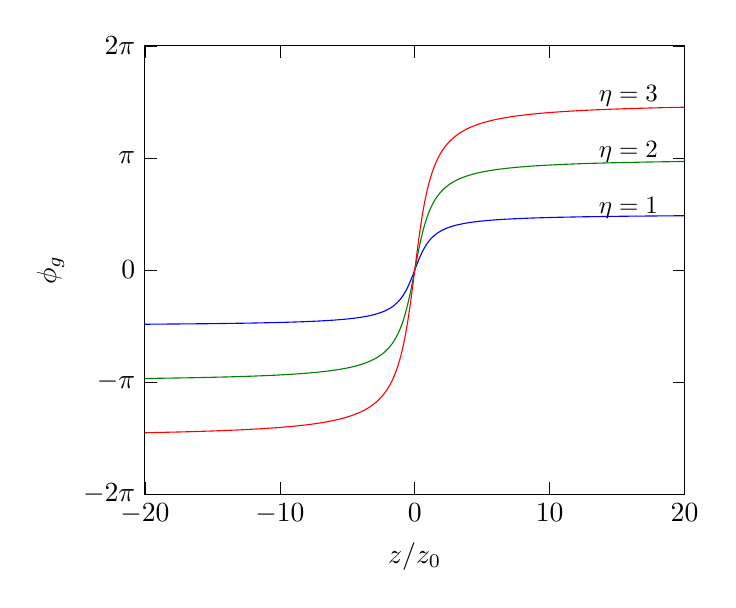
\begin{tikzpicture}

\definecolor{green01270}{RGB}{0,127,0}

\begin{axis}[
axis on top,
tick pos=both,
xlabel=\textcolor{black}{\(\displaystyle z/z_0\)},
xmin=-20, xmax=20,
xtick style={color=black},
ylabel=\textcolor{black}{\(\displaystyle \phi_g\)},
ymin=-6.28318530717959, ymax=6.28318530717959,
ytick style={color=black},
ytick={-6.28318530717959,-3.14159265358979,0,3.14159265358979,6.28318530717959},
yticklabels={
  \(\displaystyle -2\pi\),
  \(\displaystyle -\pi\),
  0,
  \(\displaystyle \pi\),
  \(\displaystyle 2\pi\)
}
]
\addplot [blue]
table {%
-20 -1.52083790302277
-15.3553552627563 -1.50576424598694
-12.1921920776367 -1.48895978927612
-9.90991020202637 -1.47022771835327
-8.22822856903076 -1.44985663890839
-6.94694709777832 -1.4278302192688
-5.94594573974609 -1.40417385101318
-5.14514493942261 -1.37883162498474
-4.46446466445923 -1.35044240951538
-3.90390396118164 -1.32003426551819
-3.46346354484558 -1.28971230983734
-3.06306314468384 -1.25523495674133
-2.74274277687073 -1.22117578983307
-2.46246242523193 -1.18504452705383
-2.22222232818604 -1.1479424238205
-1.98198199272156 -1.10351896286011
-1.78178179264069 -1.05936765670776
-1.62162160873413 -1.01821196079254
-1.46146142482758 -0.970721483230591
-1.30130136013031 -0.915584087371826
-1.14114117622375 -0.851221561431885
-1.02102100849152 -0.795799016952515
-0.900900840759277 -0.733312606811523
-0.780780792236328 -0.662911534309387
-0.660660743713379 -0.583832979202271
-0.540540456771851 -0.495551705360413
-0.420420408248901 -0.397985339164734
-0.300300359725952 -0.291732311248779
-0.140140175819397 -0.139233350753784
0.300300359725952 0.291732311248779
0.420420408248901 0.397985339164734
0.540540456771851 0.495551705360413
0.660660743713379 0.583832979202271
0.780780792236328 0.662911534309387
0.900900840759277 0.733312606811523
1.02102100849152 0.795799016952515
1.14114117622375 0.851221561431885
1.2612612247467 0.900425910949707
1.42142140865326 0.957711100578308
1.58158159255981 1.00698018074036
1.74174177646637 1.04961013793945
1.94194197654724 1.0952615737915
2.14214205741882 1.13404130935669
2.3823823928833 1.17338263988495
2.66266274452209 1.21153140068054
2.98298287391663 1.24733531475067
3.34334325790405 1.28016376495361
3.7437436580658 1.3097779750824
4.22422409057617 1.33834564685822
4.78478479385376 1.36476612091064
5.4654655456543 1.3898309469223
6.3063063621521 1.413534283638
7.34734725952148 1.43552398681641
8.66866874694824 1.45594596862793
10.3503503799438 1.47448015213013
12.5525522232056 1.49129915237427
15.4754753112793 1.50626766681671
19.5195198059082 1.51961028575897
20 1.52083790302277
};
\addplot [green01270]
table {%
-20 -3.04167580604553
-16.5965957641602 -3.02123165130615
-13.9939937591553 -2.99891662597656
-11.9519519805908 -2.97464489936829
-10.3503503799438 -2.94896030426025
-9.02902889251709 -2.9209840297699
-7.94794797897339 -2.89127063751221
-7.06706714630127 -2.86045622825623
-6.3063063621521 -2.827068567276
-5.66566562652588 -2.79218769073486
-5.10510492324829 -2.75472640991211
-4.62462472915649 -2.71568250656128
-4.22422409057617 -2.67669129371643
-3.86386394500732 -2.635089635849
-3.54354357719421 -2.59149122238159
-3.26326322555542 -2.54688048362732
-2.98298287391663 -2.49467062950134
-2.74274277687073 -2.44235157966614
-2.54254245758057 -2.39214587211609
-2.34234237670898 -2.3345959186554
-2.18218207359314 -2.28219437599182
-2.02202200889587 -2.22302937507629
-1.86186182498932 -2.15582704544067
-1.74174177646637 -2.09922027587891
-1.62162160873413 -2.03642392158508
-1.50150156021118 -1.96651077270508
-1.38138139247894 -1.88840198516846
-1.2612612247467 -1.8008519411087
-1.14114117622375 -1.70244312286377
-1.02102100849152 -1.59159791469574
-0.940940856933594 -1.50995898246765
-0.860860824584961 -1.42153131961823
-0.780780792236328 -1.32582306861877
-0.700700759887695 -1.22239220142365
-0.620620608329773 -1.1108877658844
-0.540540456771851 -0.991103410720825
-0.420420408248901 -0.795970678329468
-0.300300359725952 -0.583464622497559
-0.180180191993713 -0.356534957885742
0.0200200080871582 0.0400346517562866
0.22022020816803 0.433520674705505
0.340340375900269 0.656087160110474
0.460460424423218 0.863037347793579
0.580580592155457 1.05203628540039
0.700700759887695 1.22239220142365
0.780780792236328 1.32582306861877
0.860860824584961 1.42153131961823
0.9809809923172 1.55159533023834
1.10110116004944 1.66695845127106
1.22122120857239 1.7693305015564
1.34134137630463 1.86033415794373
1.46146142482758 1.94144308567047
1.58158159255981 2.01396036148071
1.70170176029205 2.07901883125305
1.821821808815 2.13759446144104
1.98198199272156 2.20703792572021
2.14214205741882 2.26808261871338
2.30230236053467 2.3220694065094
2.50250244140625 2.38126969337463
2.70270276069641 2.43283271789551
2.94294285774231 2.48648142814636
3.18318319320679 2.53281617164612
3.46346354484558 2.57942461967468
3.78378367424011 2.62483620643616
4.14414405822754 2.66803669929504
4.54454469680786 2.70840811729431
4.98498487472534 2.7456431388855
5.50550556182861 2.78223776817322
6.10610628128052 2.81693363189697
6.7867865562439 2.84900760650635
7.58758735656738 2.87951469421387
8.54854869842529 2.90869331359863
9.66967010498047 2.93549299240112
11.0310306549072 2.96078014373779
12.6726722717285 2.98409914970398
14.7147150039673 3.00588297843933
17.2772769927979 3.02596259117126
20 3.04167580604553
};
\addplot [red]
table {%
-20 -4.56251382827759
-17.1571578979492 -4.53773260116577
-14.8748750686646 -4.51100969314575
-13.0330333709717 -4.4826545715332
-11.5115118026733 -4.45243310928345
-10.2302303314209 -4.42006921768188
-9.14914894104004 -4.38578605651855
-8.22822856903076 -4.34956979751587
-7.46746730804443 -4.31302213668823
-6.7867865562439 -4.27351140975952
-6.18618631362915 -4.23159646987915
-5.66566562652588 -4.18828153610229
-5.2252254486084 -4.14511060714722
-4.82482481002808 -4.09928560256958
-4.46446466445923 -4.05132722854614
-4.14414405822754 -4.00205516815186
-3.86386394500732 -3.95263457298279
-3.58358359336853 -3.89600563049316
-3.34334325790405 -3.84049129486084
-3.10310316085815 -3.77713918685913
-2.90290284156799 -3.71713519096375
-2.70270276069641 -3.64924931526184
-2.54254245758057 -3.58821892738342
-2.3823823928833 -3.52014803886414
-2.22222232818604 -3.4438271522522
-2.06206202507019 -3.35777950286865
-1.94194197654724 -3.28578472137451
-1.821821808815 -3.20639157295227
-1.70170176029205 -3.11852812767029
-1.58158159255981 -3.02094054222107
-1.46146142482758 -2.91216468811035
-1.34134137630463 -2.7905011177063
-1.2612612247467 -2.7012779712677
-1.18118119239807 -2.60482048988342
-1.10110116004944 -2.50043773651123
-1.02102100849152 -2.38739681243896
-0.940940856933594 -2.26493859291077
-0.860860824584961 -2.13229703903198
-0.780780792236328 -1.98873460292816
-0.700700759887695 -1.83358824253082
-0.620620608329773 -1.6663316488266
-0.540540456771851 -1.48665499687195
-0.460460424423218 -1.29455614089966
-0.340340375900269 -0.984130620956421
-0.22022020816803 -0.650281071662903
-0.0600600242614746 -0.179964065551758
0.22022020816803 0.650281071662903
0.340340375900269 0.984130620956421
0.460460424423218 1.29455614089966
0.540540456771851 1.48665499687195
0.620620608329773 1.6663316488266
0.700700759887695 1.83358824253082
0.780780792236328 1.98873460292816
0.860860824584961 2.13229703903198
0.940940856933594 2.26493859291077
1.02102100849152 2.38739681243896
1.10110116004944 2.50043773651123
1.18118119239807 2.60482048988342
1.2612612247467 2.7012779712677
1.38138139247894 2.83260297775269
1.50150156021118 2.94976615905762
1.62162160873413 3.05463600158691
1.74174177646637 3.14883041381836
1.86186182498932 3.23374080657959
1.98198199272156 3.31055688858032
2.10210204124451 3.38029599189758
2.26226234436035 3.46375632286072
2.42242240905762 3.53788781166077
2.58258247375488 3.60409450531006
2.74274277687073 3.66352725028992
2.94294285774231 3.72972226142883
3.14314317703247 3.7883095741272
3.38338327407837 3.85024785995483
3.62362360954285 3.90459442138672
3.90390396118164 3.96010279655457
4.18418407440186 4.00860500335693
4.50450468063354 4.05701732635498
4.86486482620239 4.10419368743896
5.26526546478271 4.14932346343994
5.7057056427002 4.19188594818115
6.22622632980347 4.2346363067627
6.7867865562439 4.27351140975952
7.42742729187012 4.31089496612549
8.14814853668213 4.34603929519653
8.98898887634277 4.38001394271851
9.989990234375 4.41308546066284
11.1511507034302 4.44407606124878
12.5125122070312 4.47313737869263
14.1141138076782 4.50019025802612
16.0360355377197 4.52555227279663
18.3983974456787 4.54949140548706
20 4.56251382827759
};
\draw (axis cs:13,1.5707963267949) node[
  scale=0.9,
  anchor=base west,
  text=black,
  rotate=0.0
]{$\eta=1$};
\draw (axis cs:13,3.14159265358979) node[
  scale=0.9,
  anchor=base west,
  text=black,
  rotate=0.0
]{$\eta=2$};
\draw (axis cs:13,4.71238898038469) node[
  scale=0.9,
  anchor=base west,
  text=black,
  rotate=0.0
]{$\eta=3$};
\end{axis}

\end{tikzpicture}
}
		\caption{Variation of Gouy phase with z for HG beam}
		\label{fig:gouy_hg}
	\end{figure}
	
	
\end{enumerate}


\subsubsection{Laguerre-Gaussian beam}
In the expression \ref{eq:2.30}, we get the radially symmetric Gaussian beam solution. But we now seek higher order solution of Gaussian beam which is not radially symmetric {i.e.} vary with $\phi$.

Lets take the ansatz as,
\begin{align}
	\psi(r,\phi,z)= A \: g\left(\frac{y}{w(z)}\right) \exp\left[-i\left(p(z) + \frac{kr^2}{2q(z)}+l\phi\right)\right]
\end{align}
Putting this in Paraxial wave equation \ref{eq:2.6}, and solving the differential equation, \cite{LG}\cite{kogelnik 66} we get,
\begin{align}
	\psi_{p,l}(r,\phi,z)=&A\:\frac{w_0}{w(z)} \left[\frac{r\sqrt{2}}{w(z)}\right]^{|l|} L_p^{|l|}\left(\frac{2r^2}{w^2(z)}\right)\exp(-\frac{r^2}{w^2(z)}) \cdot\nonumber\\ &\exp(-il\phi+i(2p+l+1)\tan[-1](\frac{z}{z_0})-i\frac{kr^2}{2R(z)}) \label{eq:2.58}
\end{align}
where $l$ is \textit{vortex quantum number}, takes integer value, $ L_p^{|l|} $ is  \textit{associated Laguerre polynomial} and other terms are as usual.
\begin{figure}[!t]
	
	\foreach \n in {0,1,2}{
		\foreach \m in {0,1,2}{
				{
					\begin{subfigure}[htbp]{0.3\textwidth}
					\centering
					\includegraphics[width=\textwidth]{intensity_lg\n\m}
					\caption{$p=\n,|l|=\m$}
					%\label{fig:hg\n\m}
				\end{subfigure}
				\hfill
			}
		}
	}
	\\
	\caption{Intensity variation for different modes in a cross section ($z=0,z_0=1,w_0=1$)}
	\label{fig:lgpl}
\end{figure}

\begin{figure}[t]
	
	\foreach \n in {0,1,2}{
		\foreach \m in {0,1,2}{
			{
				\begin{subfigure}[htbp]{0.3\textwidth}
					\centering
					\includegraphics[width=\textwidth]{phase_lg\n\m}
					\caption{$p=\n,l=\m$}
					%\label{fig:hg\n\m}
				\end{subfigure}
				\hfill
			}
		}
	}
	\\
	\caption{Phase variation for different modes in a cross section ($z=0,z_0=1,w_0=1$)}
	\label{fig:phase_lgpl}
\end{figure}
Some characteristics of HG beams are given below,
\begin{enumerate}
	\item \textit{Intensity} of LG beam is given by 
	\begin{align}
		I_{p,l}(r,z)=\frac{c\epsilon}{2} |A|^2 \left[\frac{w_0}{w(z)}\right]^2 \left[\frac{r\sqrt{2}}{w(z)}\right]^{2|l|} \left[L_p^{|l|}\left(\frac{2r^2}{w^2(z)}\right) \right]^2 \exp(-\frac{2r^2}{w^2(z)})
	\end{align}
	See intensity plot for corresponding LG beam in figure \ref{fig:lgpl}. For $\abs{l}\ne 0$ the intensity of centre is zero and the value of $p$ denotes the number of radial nodes as $ L_p^{|l|} $ has $p$ number of zeros.
	
	\item 
	\textit{Rate of energy} of HG beam passes through any transverse plain is given by
	\begin{align}
		W&= \iint_{-\infty}^{\infty} dx\:dy\:I(x,y,z)\nonumber\\
		&= \frac{1}{2} \epsilon_0c \abs{A}^2 \left(\frac{w_0}{w(z)}\right)^2 \int_{-\infty}^{\infty} dx\: \left(\frac{2r^2}{w^2(z)}\right)^{\abs{l}} \left[L_p^{|l|}\left(\frac{2r^2}{w^2(z)}\right) \right]^2 \exp(-\frac{2r^2}{w^2(z)})
	\end{align}
	By same argument as HG beam, we can conclude $W$ is finite and constant throughout the propagation along z-axis
	
	\item
	\textit{Phase} of the LG beam, unlike Gaussian beam, not only depends on the $r$ and $z$, but also on $\phi$. Phase of LG beam is given by
	\begin{align}
		\Phi_{LG}(r,\phi,z) = \arg(\psi_{p,l}(r,\phi,z)) 
	\end{align}
	Phase plot for different order of LG beam at $z=0$ is given in figure \ref{fig:phase_lgpl}.
	
	\item 
	As we will see later section, unlike the HG beam, LG bream carry orbital angular momentum due to its phase variation \textit{w.r.t.} $\phi$ which results helical phase-front of the beam.
\end{enumerate}




\subsection{Maxwell-Gaussian beam (with polarization)}
According to \cite{erikson 94}, let us consider electric field $\boldsymbol{E}$ and magnetic field $\boldsymbol{E}$ of a EM wave propagating in z-direction, we write, in Cartesian coordinate,\footnote{For cylindrical coordinate, ref \cite{lewis 14}}
\begin{align}
	\boldsymbol{E}(\boldsymbol{r},t)
	&= \boldsymbol{E_0}\: e^{i(kz - \omega t)}
	= \begin{bmatrix}
		E_{0x}(\boldsymbol{r})\\E_{0y}(\boldsymbol{r})\\E_{0y}(\boldsymbol{r})
	\end{bmatrix} e^{i(kz - \omega t)}\\
	\boldsymbol{B}(\boldsymbol{r},t)
	&= \boldsymbol{B_0}\: e^{i(kz - \omega t)}
	= \begin{bmatrix}
		B_{0x}(\boldsymbol{r})\\B_{0y}(\boldsymbol{r})\\B_{0y}(\boldsymbol{r})
	\end{bmatrix} e^{i(kz - \omega t)}
\end{align}
As $\boldsymbol{E}$ and $\boldsymbol{B}$ satisfies Maxwell's equation in free space, \cite{max eq - wiki} and using $\omega/k = c$, we get,
\begin{align}
	&\nabla\cdot\boldsymbol{E}=0\\
	\Rightarrow\;& ikE_{0z}+\nabla\cdot\boldsymbol{E_0}=0\label{eq:2.65}\\
	&\nabla\cdot\boldsymbol{B}=0\\
	\Rightarrow\;& ikB_{0z}+\nabla\cdot\boldsymbol{B_0}=0\label{eq:2.67}\\
	&\nabla\times\boldsymbol{E}= -\frac{\partial \boldsymbol{B}}{\partial t}\\
	\Rightarrow\;& ik\Hat{z}\times\boldsymbol{E_0}+ \nabla\times\boldsymbol{E_0}
	=ikc\boldsymbol{B_0}\label{eq:2.69}\\
	&\nabla\times\boldsymbol{B}=\frac{1}{c^2}\frac{\partial\boldsymbol{E}}{\partial t}\\
	\Rightarrow\;& ik\Hat{z}\times\boldsymbol{B_0}+ \nabla\times\boldsymbol{B_0}
	=-ik\frac{1}{c}\boldsymbol{E_0}\label{eq:2.71}
\end{align}

Assuming paraxial approximation \ref{eq:2.6}, we get paraxial wave equation in vector form, 
\begin{align}
	\left(\frac{\partial^2}{\partial x^2}+\frac{\partial^2}{\partial y^2} + 2ik\frac{\partial}{\partial z}\right)
	\begin{Bmatrix}
		\boldsymbol{E_0}\\\boldsymbol{B_0}
	\end{Bmatrix}
	=0 \label{eq:2.72}
\end{align}
So each component of $\boldsymbol{E_0}$ and $\boldsymbol{B_0}$ will satisfy the paraxial equation. So,
\begin{align}
	\frac{\partial}{\partial z}= \frac{i}{2k}\left( \frac{\partial^2}{\partial x^2}+\frac{\partial^2}{\partial y^2}  \right) \label{eq:2.73}
\end{align}


Now considering slowly varying envelop approximation \ref{eq:2.5} for each component of $\boldsymbol{E_0}$ and $\boldsymbol{B_0}$, from \ref{eq:2.65} and \ref{eq:2.67}, we get,
\begin{align} 
	E_{0z} = \frac{i}{k}\left(\frac{\partial E_{0x}}{\partial x}+\frac{\partial E_{0y}}{\partial y}\right)\label{eq:2.74}\\
	B_{0z} = \frac{i}{k}\left(\frac{\partial B_{0x}}{\partial x}+\frac{\partial B_{0y}}{\partial y}\right)\label{eq:2.75}
\end{align}

Now putting \ref{eq:2.74} in \ref{eq:2.69}, and using \ref{eq:2.73}, matching $\boldsymbol{B_0}$ component-wise we get,
\begin{align}
	cB_{0x} &= 
	-E_{0y} + \frac{1}{2k^2}\left( \frac{\partial^2 E_{0y}}{\partial x^2} - \frac{\partial^2 E_{0y}}{\partial y^2} + 2\frac{\partial^2 E_{0x}}{\partial x\partial y} \right)\label{eq:2.76}\\
	cB_{0y} &= 
	E_{0x} + \frac{1}{2k^2}\left( \frac{\partial^2 E_{0x}}{\partial y^2} - \frac{\partial^2 E_{0x}}{\partial x^2} - 2\frac{\partial^2 E_{0y}}{\partial x\partial y} \right)\\
	cB_{0z} &= 
	\frac{i}{k}\left(\frac{\partial\: cB_{0x}}{\partial x}+\frac{\partial\: cB_{0y}}{\partial y}\right)= \frac{i}{k}\left(\frac{\partial E_{0x}}{\partial y}-\frac{\partial E_{0y}}{\partial x}\right)
\end{align}

Similarly, putting \ref{eq:2.75} in \ref{eq:2.69}, and using \ref{eq:2.73}, matching $\boldsymbol{E_0}$ component-wise we get,
\begin{align}
	\frac{1}{c}E_{0x} &=
	 B_{0y} + \frac{1}{2k^2}\left( \frac{\partial^2 B_{0y}}{\partial x^2} - \frac{\partial^2 B_{0y}}{\partial y^2} - 2\frac{\partial^2 B_{0x}}{\partial x\partial y} \right)\\
	\frac{1}{c}E_{0y} &= 
	-B_{0x} + \frac{1}{2k^2}\left( \frac{\partial^2 B_{0x}}{\partial x^2} - \frac{\partial^2 B_{0x}}{\partial y^2} + 2\frac{\partial^2 B_{0y}}{\partial x\partial y} \right)\\
	\frac{1}{c}E_{0z} &= \frac{i}{ck}\left(\frac{\partial E_{0x}}{\partial x}+ \frac{\partial E_{0y}}{\partial y}\right) = \frac{i}{k}\left(\frac{\partial B_{0y}}{\partial x}-\frac{\partial B_{0x}}{\partial y}\right)\label{eq:2.81}
\end{align}

Let $\psi_x(\boldsymbol{r})$ and $\psi_y(\boldsymbol{r})$ are the dominant x and y component of electric field satisfying paraxial wave equation. If we write magnetic field component as \cite{erikson 94}
\begin{align}
	cB_{0x} &= 
	-\psi_y + \frac{1}{4k^2}\left( \frac{\partial^2 \psi_y}{\partial x^2} - \frac{\partial^2 \psi_y}{\partial y^2} + 2\frac{\partial^2 \psi_x}{\partial x\partial y} \right)\label{eq:2.85}\\
	cB_{0y} &= 
	\psi_x + \frac{1}{4k^2}\left( \frac{\partial^2 \psi_x}{\partial y^2} - \frac{\partial^2 \psi_x}{\partial x^2} - 2\frac{\partial^2 \psi_y}{\partial x\partial y} \right)\\
	cB_{0z} &= 
	\frac{i}{k}\left(\frac{\partial \psi_x}{\partial y}-\frac{\partial \psi_y}{\partial x}\right)
\end{align}
and electric field component as \cite{erikson 94}
\begin{align}
	E_{0x} &=
	\psi_x + \frac{1}{4k^2}\left( \frac{\partial^2 \psi_x}{\partial x^2} - \frac{\partial^2 \psi_x}{\partial y^2} + 2\frac{\partial^2 \psi_y}{\partial x\partial y} \right)\\
	E_{0y} &= 
	\psi_y - \frac{1}{4k^2}\left( \frac{\partial^2 \psi_y}{\partial x^2} - \frac{\partial^2 \psi_y}{\partial y^2} + 2\frac{\partial^2 \psi_x}{\partial x\partial y} \right)\\
	E_{0z} &= 
	\frac{i}{k}\left(\frac{\partial \psi_x}{\partial x}+\frac{\partial \psi_y}{\partial y}\right)\label{eq:2.90}
\end{align}
then the eq. \ref{eq:2.85} - \ref{eq:2.90} satisfy the paraxial Maxwell's relations \ref{eq:2.76} - \ref{eq:2.81} up-to the order of $1/(kw_0)^2$, where $w_0$ is Rayleigh length of Gaussian beam.


Now we will consider two cases of polarization for HG beam - linear and circular polarization.
\begin{enumerate}
	\item 
	\textbf{Linear polarization}\\
	Let the dominant polarization is in x direction, then $\psi_x=\psi_{m,n}$ of \ref{eq:2.53} and $\psi_y=0$. The electric field components are
	\begin{align}
		E_{0x} =&
		\psi_{m,n}\\
		E_{0y} =& 
		\frac{1}{2k^2}\frac{\partial^2 \psi_{m,n}}{\partial x\partial y}\nonumber \\
		=&\frac{1}{4k^2w_0^2} \big( 4mn\psi_{m-1,n-1} - 2m\psi_{m-1,n+1} - 2n\psi_{m+1,n-1} + \psi_{m+1,n+1}\big)\\
		E_{0z} =& 
		\frac{i}{k}\frac{\partial \psi_{m,n}}{\partial x}\nonumber\\
		=& \frac{i}{\sqrt{2}kw_0}\big(2m\psi_{m-1,n} - \psi_{m+1,n}\big)
	\end{align}
	Here we use the the following properties of Hermite polynomials, \cite{levedev} \textit{i.e.} $\forall x\in \mathbb{R}$ and $\forall n\in \mathbb{N}$, 
	\begin{align}
		H_{n+1}(x) &= 2x H_n(x) - 2nH_{n-1}(x)\label{eq:2.91}\\
		\frac{d}{dx}H_n(x)&=2nH_{n-1}(x)\label{eq:2.92}
	\end{align}
	
	\item 
	\textbf{Circular polarization}\\
	Similarly for LCP, $\psi_x=\psi_{m,n}$ and $\psi_y=i\psi_{m,n}$, the electric field components, using \ref{eq:2.91} and \ref{eq:2.92}, are
	\begin{align}
		E_{0x} =&
		\frac{1}{\sqrt{2}}\psi_{m,n}\\
		E_{0y} =& 
		\frac{i}{\sqrt{2}}\psi_{m,n}\\
		E_{0z} =& 
		\frac{i}{2kw_0}\big( 4m\psi_{m-1,n} - \psi_{m+1,n} + i2n\psi_{m,n-1} - i\psi_{m,n+1}\big)
	\end{align}
\end{enumerate}

\subsection{Relationship between LG \& HG modes}
According to \cite{abra 91}, for $n,m = 0,1,2,\dots$
\begin{align}
	&\sum_{k=0}^{n+m}(2i)^k \mathcal{P}_k^{(n-k,m-k)}(0)H_{n+m-k}(x)H_k(y)\nonumber\\
	&=
	\begin{cases}
		2^{n+m}(-1)^m m! (x+iy)^{n-m}L_m^{n-m}(x^2+y^2),& n\ge m\\
		2^{n+m}(-1)^n n! (x+iy)^{m-n}L_n^{m-n}(x^2+y^2),& m > n
	\end{cases}
\end{align}
where
\begin{align}
	\mathcal{P}_k^{(n-k,m-k)}(0) = \frac{(-1)^k}{2^kk!} \frac{d^k}{dt^k}\big[(1-t)^n(1+t)^m \big] \bigg|_{t=0}
\end{align}

Now the scalar field representations of HG and LG beam are 
\begin{align}
	U_{m,n}^{HG}(x,y,z)=& \frac{C_{m,n}^{HG}}{w(z)} H_m\left(\frac{\sqrt{2} x}{w(z)}\right) H_n\left(\frac{\sqrt{2} y}{w(z)}\right)\exp( -\frac{(x^2+y^2)}{w^2(z)}) \cdot\nonumber\\ 
	&\exp( i\:(m+n+1)\eta -i\frac{k(x^2+y^2)}{2R(z)}) \\
	U_{n,m}^{LG}(x,y,z)=&(-1)^{\min(n,m)}\frac{C_{m,n}^{LG}}{w(z)} \left[\frac{\sqrt{2(x^2+y^2)}}{w(z)}\right]^{|n-m|} L_{\min(n,m)}^{|n-m|}\left(\frac{2(x^2+y^2)}{w^2(z)}\right)\cdot\nonumber\\&\exp(-\frac{(x^2+y^2)}{w^2(z)}) \exp(-i(n-m)\arg(x+iy)-i(n+m-1)\eta-i\frac{kr^2}{2R(z)}) 
\end{align}
where\footnote{here $w(z)$ is not the beam half-width but scaled version of that.}
\begin{align}
	R(z)&= \frac{z_0^2+z^2}{z}\\
	w(z)&= \sqrt{\frac{2(z_0^2+z^2)}{kz}}\\
	\eta(Z)&= \tan[-1](\frac{z}{z_0})
\end{align}
and the normalization constants, such that $\iint dx\:dy\: \abs{U}=1$, are
\begin{align}
	C_{m,n}^{HG}=\sqrt{\frac{2}{\pi n!m!}}2^{-(m+n)/2}\\
	C_{m,n}^{LG}=\sqrt{\frac{2}{\pi n!m!}}\min(n,m)!
\end{align}
Here to get the LG beam representation, use $l=n-m$ and $p=\min(n,m)$ in \ref{eq:2.58}.

Using this identity, the LG beam can be decomposed into various order of HG beam by, \cite{beijers allen 93}
\begin{align}
	U_{m,n}^{LG}= \sum_{k=0}^{n+m}i^k b(n,m,k)\: U_{m+n-k,k}^{HG}
\end{align}
where,
\begin{align}
	b(n,m,k)=\frac{1}{k!}\sqrt{\frac{(n+m)!k!}{2^{n+m}n!m!}} \frac{d^k}{dt^k}\big[(1-t)^n(1+t)^m \big] \bigg|_{t=0}
\end{align}
\clearpage


\section{MOMENTUM OF LIGHT}
\subsection{Introduction}
We know EM wave carries energy as well as momentum. Momentum can be two types, linear and angular momentum. The \textit{momentum density} of EM wave is momentum per unit volume.

\subsection{Linear and angular momentum of light}
If linear momentum density is $\boldsymbol{p}$ and linear momentum is $\boldsymbol{P}$ then,
\begin{align}
	\boldsymbol{p} &= \frac{1}{c^2}\boldsymbol{S} = \epsilon_0 \boldsymbol{E} \times \boldsymbol{B}\label{eq:3.1}\\
	\boldsymbol{P} &= \int \boldsymbol{p} \:d\tau \label{eq:3.2}
\end{align}

Now let the monochromatic field with angular frequency $\omega$, then
\begin{align}
	\boldsymbol{\mathcal{E}}(\boldsymbol{r},t) &= \Re{\boldsymbol{E}(\boldsymbol{r}) e^{-i \omega t }} = \frac{1}{2}(\boldsymbol{E} e^{-i \omega t } +\boldsymbol{E}^\ast e^{i \omega t})\\
	\boldsymbol{\mathcal{B}}(\boldsymbol{r},t) &= \Re{\boldsymbol{B}(\boldsymbol{r}) e^{-i \omega t }} = \frac{1}{2}(\boldsymbol{B} e^{-i \omega t } +\boldsymbol{B}^\ast e^{i \omega t})
\end{align}

From Maxwell-Faraday equation in free space, we know that, \cite{haus}
\begin{align}
	\nabla\times\boldsymbol{\mathcal{E}}&= - \frac{\partial}{\partial t}\boldsymbol{\mathcal{B}}\\
	\Rightarrow \nabla\times\boldsymbol{E}&= i\omega \boldsymbol{B} \label{eq:3.6}
\end{align}

The total energy is given by
\begin{align}
	W = \int d\tau\: \frac{I}{c}=\frac{\epsilon_0}{2}\int d\tau\: \boldsymbol{E}^\ast\cdot\boldsymbol{E}
\end{align}

Now time-averaged Poynting vector is given by, \cite{poynting}\cite{haus}
\begin{align}
	\expval{\boldsymbol{S}} =\frac{1}{\mu_0}\expval{\boldsymbol{\mathcal{E}} \times \boldsymbol{\mathcal{B}}} =\frac{1}{\mu_0}\; \frac{1}{2} \Re{\boldsymbol{E}^\ast \times \boldsymbol{B}} \label{eq:3.8}
%=\frac{1}{2\mu_0}\:(\boldsymbol{E}^\ast \times \boldsymbol{B}+ \boldsymbol{E} \times \boldsymbol{B}^\ast )
\end{align}

From eq. \ref{eq:3.1} and \ref{eq:3.2} and using \ref{eq:3.6} and \ref{eq:3.8}, time-averaged linear momentum is given by
\begin{align}
	\boldsymbol{P} &= \frac{1}{c^2}\int d\tau\: \expval{\boldsymbol{S}}\\
	&=\frac{\epsilon_0}{2}\int d\tau \:\Re{\boldsymbol{E}^\ast \times \boldsymbol{B}}\nonumber\\
	&= \frac{\epsilon_0}{2i\omega}\int d\tau\: \Re{\boldsymbol{E}^\ast \times (\nabla\times\boldsymbol{E})} 
\end{align}
On partial integration and using the transversality of E, considering the magnitude of $\boldsymbol{E}$ decreasing very rapidly when $r\to0$, \cite{enk nien 92} we get\footnote{see derivation in Chapter I in ref. \cite{CCT}}
\begin{align}
	\boldsymbol{P}= \frac{\epsilon_0}{2i\omega}\int d\tau \left[\sum_{\xi=x,y,z}E_\xi^\ast\nabla E_\xi\right]
\end{align}
which is quantum mechanical equivalent for linear momentum of a particle.


Let angular momentum density is $\boldsymbol{j}$ and angular momentum is $\boldsymbol{J}$ then,
\begin{align}
	\boldsymbol{j} &= \frac{1}{c^2}\boldsymbol{r}\times\boldsymbol{S} = \epsilon_0 \boldsymbol{r}\times(\boldsymbol{E} \times \boldsymbol{B})\label{eq:3.12}\\
	\boldsymbol{J} &= \int \boldsymbol{j} \:d\tau\label{eq:3.13}
\end{align}

Similarly from eq. \ref{eq:3.12} and \ref{eq:3.13} and using \ref{eq:3.6} and \ref{eq:3.8}, time-averaged angular momentum, 
\begin{align}
	\boldsymbol{J} &= \frac{1}{c^2}\int d\tau\: \boldsymbol{r}\times\expval{\boldsymbol{S}}\\
	&=\frac{\epsilon_0}{2}\int d\tau \:\boldsymbol{r}\times\Re{\boldsymbol{E}^\ast \times \boldsymbol{B}}\nonumber\\
	&= \frac{\epsilon_0}{2i\omega}\int d\tau\: \Re{\boldsymbol{r}\times\left(\boldsymbol{E}^\ast \times (\nabla\times\boldsymbol{E})\right)}
\end{align}

Now similarly on partial integration and using the transversality of E, considering the magnitude of $\boldsymbol{E}$ decreasing very rapidly when $r\to0$, \cite{enk nien 92}\cite{allen 99} we get\footnote{see derivation in Chapter I in ref. \cite{CCT}}

\begin{align}
	 \boldsymbol{J}=\frac{\epsilon_0}{2i\omega}\int d\tau \left[\sum_{\xi=x,y,z}E_\xi^\ast(\boldsymbol{r}\times\nabla)E_\xi\right]+ \frac{\epsilon_0}{2i\omega}\int d\tau \boldsymbol{E}^\ast\times \boldsymbol{E}
\end{align}

Now according to \cite{bernatt allen 94} \& \cite{enk nien 92}, within the paraxial approximation, to get time-averaged energy, linear momentum and angular momentum per unit length \textit{i.e.} $\mathcal{W}$, $\mathcal{P}$ and $\mathcal{J}$ respectively, along the beam propagating in z-direction, we have to integrate throughout the transverse xy-plane. So,
\begin{align}
	\mathcal{W}_z&=\frac{\epsilon_0}{2}\iint dx\:dy\: \boldsymbol{E}^\ast\cdot\boldsymbol{E}\label{eq:3.17}\\
	\mathcal{P}_z&=\frac{\epsilon_0}{2i\omega}\iint  dx\:dy\: \expval{\boldsymbol{E}\times (\nabla\times\boldsymbol{E})}_z\\
	\mathcal{J}_z&=\frac{\epsilon_0}{2i\omega}\iint dx\:dy\: \left[\boldsymbol{r}\times\expval{\boldsymbol{E}\times (\nabla\times\boldsymbol{E})}\right]_z
	\label{eq:3.19}
\end{align}


\subsection{More on angular momentum}
Let the electric field of the paraxial EM wave is \cite{WO} 
\begin{align}
	\boldsymbol{E}(x,y,z)=\boldsymbol{F}(x,y,z)\:e^{ikz} \label{eq:3.20}
\end{align}
\textit{s.t.} $\boldsymbol{F}$ is the slowly varying spatial envelop, satisfies the paraxial wave equation \ref{eq:2.6} \textit{i.e.}
$$\nabla_T ^2\boldsymbol{F} +2ik \frac{\partial\boldsymbol{F}}{\partial r}=0$$
also assumed that the beam waist $w_0$ (transverse dimension of the beam) is
assumed to be much smaller than the diffraction length, $l_d = kw_0^2$ and z- component of $\boldsymbol{F}$ is smaller than transverse component by a factor of $w_0/l_d$. \cite{melvin 75}\cite{enk nien 92}\cite{WO}

From previous eq. \ref{eq:3.19}, z-component of $\mathcal{J}$ for \ref{eq:3.20} is given by

\begin{align}
	\mathcal{J}_z (z)
	= \underbrace{\frac{\epsilon_0}{2i\omega} \iint dx\:dy\:\left[F_\xi^\ast\left(x\frac{\partial}{\partial y} - y\frac{\partial}{\partial x}\right)F_\xi\right]_{\xi=x,y}}_{\text{1st term }}
	+\underbrace{\frac{\epsilon_0}{2i\omega}\iint dx\:dy\: (F_x^\ast F_y + F_y^\ast F_x)}_{\text{2nd term}} \label{eq:3.21}
\end{align}

Note that, in \ref{eq:3.21}, we can separately identify two terms. According to \cite{WO}, the first is associated with transverse distribution of electric field (amplitude and phase) as 
$x\frac{\partial}{\partial y} - y\frac{\partial}{\partial x}$
is equivalent to $\frac{\partial}{\partial\phi}$ in cylindrical coordinate and the second term to the polarization of electric field. Thus it is concluded,\cite{enk nien 92} within the paraxial approximation, that
\begin{enumerate}
	\item 
	first term is the orbital angular momentum (OAM) per unit length in z of the EM wave,
	\begin{align}
		\mathcal{L} &= \frac{\epsilon_0}{2i\omega} \iint dx\:dy\:\left[F_\xi^\ast\left(x\frac{\partial}{\partial y} - y\frac{\partial}{\partial x}\right)F_\xi\right]_{\xi=x,y}\nonumber\\
		&=\frac{\epsilon_0}{2i\omega} \iint dx\:dy\:\left[F_\xi^\ast\left(\boldsymbol{r}\times\nabla\right)_zF_\xi\right]_{\xi=x,y}\label{eq:3.22}
	\end{align}
	which is quantum mechanical equivalent of z-component of the angular momentum of a particle.
	
	\item 
	second term is the spin angular momentum (SAM) per unit length in z,
	\begin{align}
		\mathcal{S} = \frac{\epsilon_0}{2i\omega}\iint dx\:dy\: (F_x^\ast F_y + F_y^\ast F_x) \label{eq:3.23}
	\end{align}
\end{enumerate}
\subsubsection{Orbital and spin Angular Momentum}
Let envelop $\boldsymbol{F}$ corresponding to the EM wave \ref{eq:3.20} for a vortex beam (\textit{e.g.} LG beam) be,
\begin{align}
	\boldsymbol{F}(r,\phi)= u(r)\:\exp(-il\phi)\:\Hat{\boldsymbol{p}}
\end{align} where $e^{il\phi}$ refers to helical phase front, and $\Hat{\boldsymbol{p}} = p_x\Hat{x}+ p_y\Hat{y}+p_z\Hat{z}$ refers to unit polarization direction of electric field. Putting it in \ref{eq:3.22} considering $x\frac{\partial}{\partial y} - y\frac{\partial}{\partial x} \equiv \frac{\partial}{\partial\phi}$, we get,
\begin{align}
	\mathcal{L}&=\frac{\epsilon_0}{2i\omega} \iint r\:dr\:d\phi\:\left[F_\xi^\ast\frac{\partial}{\partial\phi}F_\xi\right]_{\xi=x,y}\nonumber\\
	&= 	\frac{\epsilon_0}{2\omega} l \left(\abs{p_x}^2+\abs{p_y}^2\right)2\pi \int r\:dr\:\abs{u(r)}^2 \nonumber
\end{align}
considering z-component of $\Hat{\boldsymbol{p}}$ is smaller than transverse component by a factor of $w_0/l_d$, so $\abs{p_x}^2+\abs{p_y}^2 \approx \abs{p_x}^2+\abs{p_y}^2+\abs{p_z}^2 = \abs{\Hat{\boldsymbol{p}}}^2 = 1$, then
\begin{align}
	\mathcal{L}=\frac{\pi\epsilon_0l}{\omega}\int r\:dr\:\abs{u(r)}^2 \label{eq:3.25}
\end{align}

For the SAM part \ref{eq:3.23},
\begin{align}
	\mathcal{S} &= \frac{\epsilon_0}{2i\omega}\iint r\:dr\:d\phi\: (F_x^\ast F_y + F_y^\ast F_x)\nonumber\\
	&=\frac{\epsilon_0}{2i\omega} (p_x^\ast p_y- p_y^\ast p_x)2\pi \int r\:dr\: \abs{u(r)}^2
\end{align}
let us define a term \textit{polarization helicity} $\sigma$ as 
\begin{align}
	\sigma = 2\Im(p_x^\ast\: p_y) = \frac{1}{i} (p_x^\ast p_y- p_y^\ast p_x)
\end{align}
then
\begin{align}
	\mathcal{S}
	=\frac{\pi\epsilon_0\sigma }{\omega}\int r\:dr\: \abs{u(r)}^2 \label{eq:3.28}
\end{align}

The relation between polarization direction $\Hat{\boldsymbol{p}}$ and Jones vector $\boldsymbol{J}$ is\footnote{for fully polarized light only} 
	\begin{align}
		\Hat{\boldsymbol{p}} = \boldsymbol{J} e^{i\omega t}
	\end{align}

So
\begin{align}
	\sigma = \frac{1}{i}(p_x^\ast p_y- p_y^\ast p_x)
	=\frac{1}{i}(J_x^\ast J_y- J_y^\ast J_x)
\end{align}

Using table \ref{table:1},
\begin{enumerate}
	\item For LCP, $\sigma = \frac{1}{2i}(1i+1i)=1$
	\item For RCP, $\sigma = \frac{1}{2i}(-1i-1i)=-1$
	\item for linearly polarized, $\sigma = \frac{1}{i}(1-1)=0$, so no SAM.
\end{enumerate}

Now for $\mathcal{W}$ in \ref{eq:3.17}, we get,
\begin{align}
	\mathcal{W}_z &=\frac{\epsilon_0}{2}\iint r\:dr\:d\phi\: \boldsymbol{E}^\ast\cdot\boldsymbol{E}\nonumber\\
	&= \frac{\epsilon_0}{2}\iint r\:dr\:d\phi\: \boldsymbol{F}^\ast\cdot\boldsymbol{F}\nonumber\\
	&=\frac{\epsilon_0}{2} \left(\abs{p_x}^2+\abs{p_y}^2+\abs{p_z}^2\right) 2\pi\int r\:dr\:\abs{u(r)}^2\nonumber\\
	&=\pi\epsilon_0\int r\:dr\:\abs{u(r)}^2 \label{eq:3.31}
\end{align}

See from \ref{eq:3.25} and \ref{eq:3.31}, 
\begin{align}
	\frac{\mathcal{L}}{\mathcal{W}_z} = \frac{l}{\omega} =\frac{\text{OAM}}{\text{Total energy}} \label{eq:3.32}
\end{align}
from \ref{eq:3.28} and \ref{eq:3.31},
\begin{align}
	\frac{\mathcal{S}}{\mathcal{W}_z} = \frac{\sigma}{\omega} =\frac{\text{SAM}}{\text{Total energy}}\label{eq:3.33}
\end{align}
and from \ref{eq:3.32} and \ref{eq:3.33},
\begin{align}
	\frac{\mathcal{J}_z}{\mathcal{W}_z} = \frac{\mathcal{L}+\mathcal{S}}{\mathcal{W}_z} = \frac{l+\sigma}{\omega} =\frac{\text{Total AM}}{\text{Total energy}} \label{eq:3.34}
\end{align}

We know for a photon the energy associated with it is $\hbar\omega$, then from \ref{eq:3.32} and \ref{eq:3.33}, we can say, the OAM associated with one photon of paraxial vortex beam is $l\hbar$ and SAM associated with one photon is $\sigma\hbar$.

\subsubsection{Intrinsic and Extrinsic nature of angular momentum}
If we observe the expression of $\mathcal{J}_z$ in \ref{eq:3.19}, it may depends on the choice of the axis (usually $\boldsymbol{r} = (0,0) $), from which we measure $\boldsymbol{r}$. \cite{WO}\cite{berry 98} But if we shift the $\boldsymbol{r}$ \textit{s.t.}
\begin{align}
	\boldsymbol{r}&\longrightarrow\boldsymbol{r'}=\boldsymbol{r}+\boldsymbol{r_0}\\
	(x,y)&\longrightarrow(x',y')=(x,y)+(x_0,y_0)
\end{align}
then change of $\mathcal{J}_z$ will be
\begin{align}
	\mathcal{J}_z\longrightarrow\mathcal{J'}_z = \mathcal{J}_z +  (\boldsymbol{r_0}\times\mathcal{P})\cdot\Hat{z}
\end{align}
The change in angular momentum,
\begin{align}
	\Delta\mathcal{J}_z&= \mathcal{J'}_z-\mathcal{J}_z = (\boldsymbol{r_0}\times\mathcal{P})\cdot\Hat{z}\\
	\Rightarrow\Delta\mathcal{J}_z&= \frac{x_0\epsilon_0}{2}\iint  dx\:dy\: \expval{\boldsymbol{E}\times\boldsymbol{B}}_y + \frac{y_0\epsilon_0}{2}\iint  dx\:dy\: \expval{\boldsymbol{E}\times\boldsymbol{B}}_x \label{}
\end{align}

Now, we say the AM is \textit{intrinsic}, when the AM does not depends on the choice of the reference axis, and \textit{extrinsic} when it depends on the choice of axis.

If the AM is to be intrinsic, then for all $(x_0,y_0)$
\begin{align}
	&\Delta\mathcal{J}=0\nonumber\\
	\Rightarrow &\iint  dx\:dy\: \expval{\boldsymbol{E}\times\boldsymbol{B}}_y = 0 = \iint  dx\:dy\: \expval{\boldsymbol{E}\times\boldsymbol{B}}_x \label{eq:3.40}
\end{align} 

From the SAM part, we see $\mathcal{S}$ does not depend on the choice of the axis, so SAM is intrinsic. But for the OAM part, we see $\mathcal{L}$ depends on the choice of the axis, so OAM may be intrinsic or extrinsic determined by, (from \ref{eq:3.22})
\begin{align}
	\Delta \mathcal{L}=
	\iint  dx\:dy\: \left[F_\xi^\ast\left(\boldsymbol{r_0}\times\nabla\right)_zF_\xi\right] = 0, \;\text{where}\;\xi=x,y
\end{align}


\subsection{\color{red} Observation of AM of light}
\cite{yao 11} pg- 176

\clearpage

\section{SPIN-ORBIT INTERACTION}

\subsection{Introduction}
The interaction between light and matter is a fascinating realm of physics. One crucial of this interaction is the spin-orbit interaction on light. The underlying framework is the interaction between the spin and  orbital angular momentum of light. In this section, we will briefly discuss about that.
\subsection{Spin-orbit energy}
In quantum mechanics, spin-orbit interaction is a common phenomena. We can see it in the splitting of spectral lines into fine structure. For a simple case like H atom, a electron in orbit around the nucleus, the spin-orbit coupling results from the interaction between electron's spin magnetic moment and nucleus's orbital magnetic field, which we will discuss below. \cite{WO}\cite{zettili 09} 

The spin magnetic moment of a electron is given by
\begin{align}
	\boldsymbol{\mu_s}=-\frac{e}{m_ec}\boldsymbol{S}
\end{align}
where $e$, $m_e$ are absolute charge and mass of electron respectively and $\boldsymbol{S}$ is spin angular momentum of electron.

For our system, the electric field is centrally symmetric \textit{i.e.}
\begin{align}
	\boldsymbol{E}= -\frac{1}{e}\frac{dU}{dr}\Hat{\boldsymbol{r}}= -\frac{1}{er}\frac{dU}{dr}\boldsymbol{r}
\end{align} where $U$ is the potential energy, 
\begin{align}
	U = \frac{1}{4\pi\epsilon_0}\frac{e^2}{r}
\end{align}

Now if electron rotates around the nucleus with instantaneous velocity $\boldsymbol{v}$, then from the rest frame of electron, the nucleus is rotating with $-\boldsymbol{v}$ around the electron thus creating a magnetic field in centre, which is\footnote{the coefficient $1/c$ is in cgs, but $1/c^2$ in SI. \cite{relativity -wiki}} 
\begin{align}
	\boldsymbol{B} = -\frac{1}{c} \boldsymbol{v}\times\boldsymbol{E} = -\frac{1}{m_ec}\boldsymbol{E}\times\boldsymbol{P}
\end{align}where $\boldsymbol{P}=m_e\boldsymbol{v}$ is momentum.

Due to spin-orbit interaction, the corresponding interaction energy rises,
\begin{align}
	H_{so}= -\boldsymbol{\mu_s}\cdot \boldsymbol{B} = -\frac{e}{m_ec}\boldsymbol{S}\cdot\boldsymbol{B} =
	-\frac{e}{m_e^2c^2}\boldsymbol{S}\cdot(\boldsymbol{E}\times\boldsymbol{P}) 
	=\frac{1}{m_e^2c^2r}\frac{dU}{dr}\boldsymbol{S}\cdot(\boldsymbol{r}\times\boldsymbol{P})
\end{align} Taking orbital angular momentum $\boldsymbol{L}=\boldsymbol{r}\times\boldsymbol{P}$, we get,
\begin{align}
	H_{so}=\frac{1}{m_e^2c^2r}\frac{dU}{dr}\boldsymbol{S}\cdot\boldsymbol{L}
\end{align}
We call $H_{so}$ as \textit{Spin-orbit energy}.\footnote{By Thomas precision, multiplication of a factor of 1/2 is necessary to agree with experimental results. It is informally known as the "Thomas half". \cite{thomas}}


\subsection{Geometric phase of light}
We know from the knowledge of waves, there is the phase factor corresponding to the EM wave due to optical path length difference, called \textit{dynamical phase}. But there is another phase factor other than dynamical one, due to the geometry or topology of the evolution of the electromagnetic wave, we call it \textit{Geometric phase}.\cite{WO} Geometric phases arises from intrinsic angular momentum and rotations of coordinates. The geometric phase and angular momentum underlie the SOI of light.\cite{bliokh 15} The two types of geometric phases, will be discussed, are
\begin{enumerate}
	\item Spin-redirection Berry phase
	\item Pancharatnam-Berry phase
\end{enumerate}

\subsubsection{Spin-redirection Berry phase}
This \textit{Berry phase} associated with adiabatic evolution of wave-vector $\boldsymbol{k}$. When the wave vector complete a adiabatic cycle, we will find a geometric phase arises from it.  As an example, let a polarized light passes through a helical optic fibre with very low (negligible) birefringence and no torsional stress\footnote{Torsional stress produces circular birefringence by elasto-optic effect. \cite{ross 84}}. After one helical patch, the $\boldsymbol{k}$ wave-vector come to the same state, but gives rise of a helicity-dependant geometric phase\footnote{This is a \textit{non-holonomic process}. \cite{anholonomy}} called \textit{spin-redirection Berry phase}. \cite{bliokh 15}

For circularly polarized light, we can write Jones vector as 
\begin{align}
	\boldsymbol{J} = 
	\begin{bmatrix}
		1\\i\sigma
	\end{bmatrix}
\end{align}
where  $\sigma$ is helicity (either $+1$ or $-1$).

Considering transversality of electric field, it will be tangent on the sphere in momentum space. And in one adiabatic cycle of wave-vector \textit{w.r.t.} $k_z$, the non-trivial parallel transport of the electric-field vectors takes place on the sphere.\cite{bliokh 15} So after transportation of a vector, the vector is rotated by an angle $\Theta$ \cite{par trans} \textit{i.e.} the frame is rotated by an angle $\Theta$ where
\begin{align}
	\Theta = 2\pi(1-\cos\theta)
\end{align} where $\theta$ is half-apex angle of the cone formed by sweeping the wave vector $\boldsymbol{k}$ in momentum space (see fig \ref{fig:berry b}). Note that $\Theta$ is the solid angle obtained at the apex of the cone.

\begin{figure}[t]
	\begin{subfigure}[H]{0.62\textwidth}
		\centering
		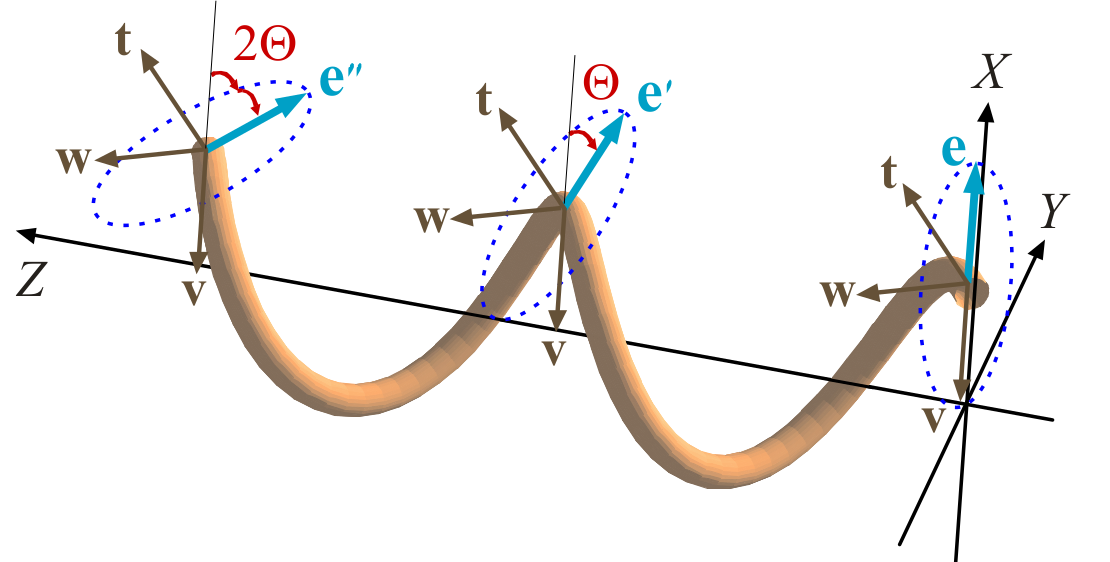
\includegraphics[width=0.9\textwidth]{berry.png}
		\caption{Evolution of polarization axis along helical optic fibre (ref. \cite{bliokh 09})}
		\label{fig:berry a}
	\end{subfigure}
	\hfil
	\begin{subfigure}[H]{0.35\textwidth}
		\centering
		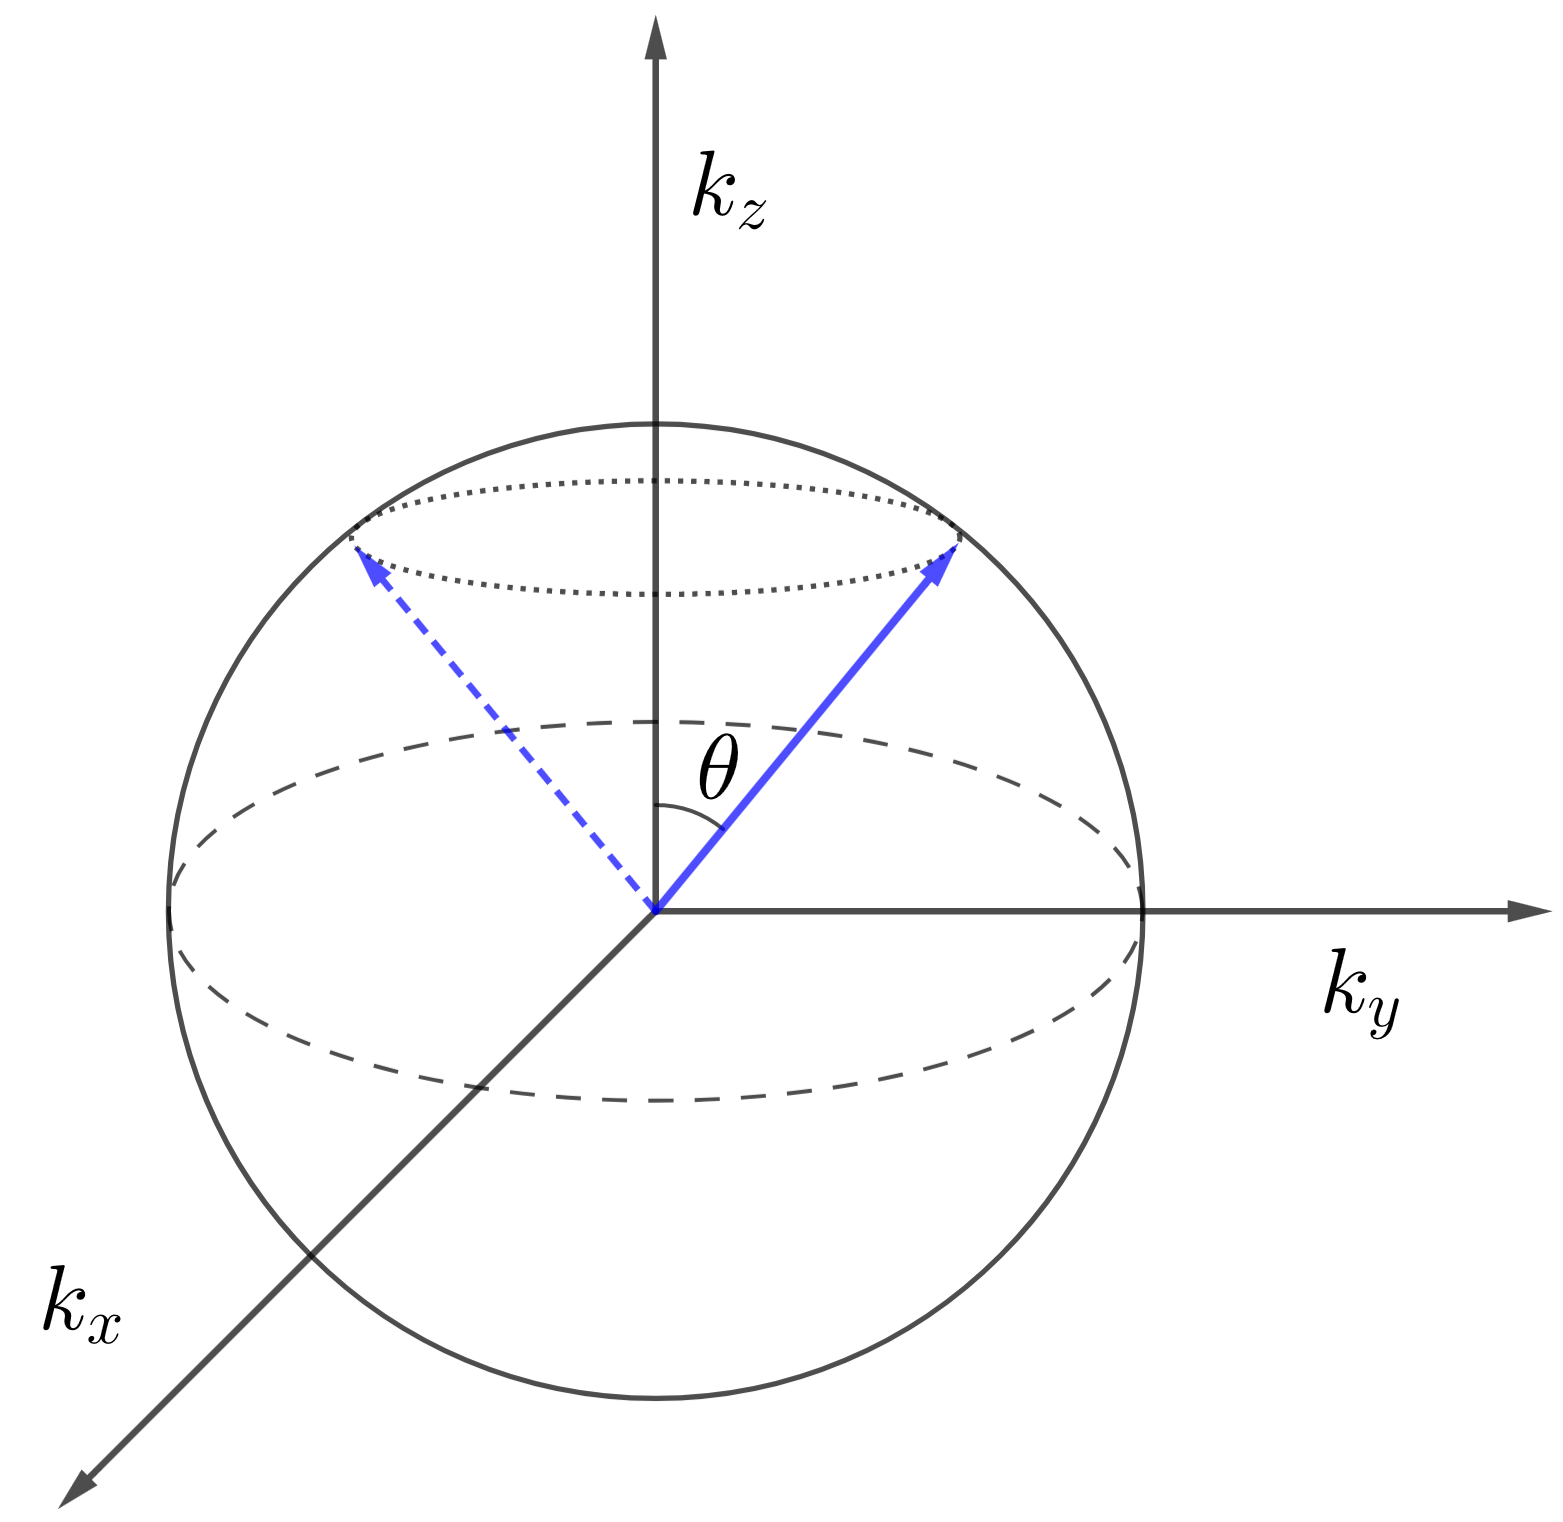
\includegraphics[width=0.9\textwidth]{poincare-berry.png}
		\caption{Evolution of wave-vector $\boldsymbol{k}$ along helical optic fibre in momentum space}
		\label{fig:berry b}
	\end{subfigure}
	\caption{Geometric Berry phase arises along helical optic fibre}
\end{figure} 

After one adiabatic cycle, electric field vector for circularly polarized light, $\boldsymbol{J}$ transform into $\boldsymbol{J'}$ where
\begin{align}
\boldsymbol{J}\longrightarrow\boldsymbol{J'}=\boldsymbol{J}\exp(i\Theta_G)
\end{align} where $\Theta_G$ is the acquired helicity-dependant geometric phase \textit{s.t.} 
\begin{align}
	\Theta_G= \sigma\Theta
\end{align}
So,
\begin{align}
	\ket{L}&\longrightarrow e^{i\Theta}\ket{L}\\
	\ket{R}&\longrightarrow e^{-i\Theta}\ket{R}
\end{align}

Now for x-polarized light, $\ket{x_{in}}$ and $\ket{x_{out}}$ will be
\begin{align}
	\ket{x_{in}} &= \frac{1}{\sqrt{2}}\left(\ket{L}+\ket{R}\right)\\
	\ket{x_{out}} &= \frac{1}{\sqrt{2}}\left(e^{i\Theta}\ket{L}+ e^{-i\Theta}\ket{R}\right)
\end{align} So the x-polarized light is rotated by angle $\Theta$ after one cycle, shown in fig \ref{fig:berry a}. Note that $\theta$ does not originate from intrinsic anisotropy and it is geometric one. We call it \textit{spin-redirection Berry phase}.

\subsubsection{Pancharatnam-Berry Phase}
Unlike the previous one, the \textit{Pancharatnam-Berry phase} arises after a cyclic evolution in Poincare sphere when the state of polarization changes  keeping wave-vector $\boldsymbol{k}$ is fixed. Convenient example of observation of Pancharatnam-Berry phase is Michelson interferometer setup, (see fig. \ref{fig:pb expt}) in which one arm of the interferometer has two quarter wave-plates, one (QP1) is fixed and another one (QP2) is rotatable. \cite{chyba 88}

\begin{figure}[H]
	\centering
	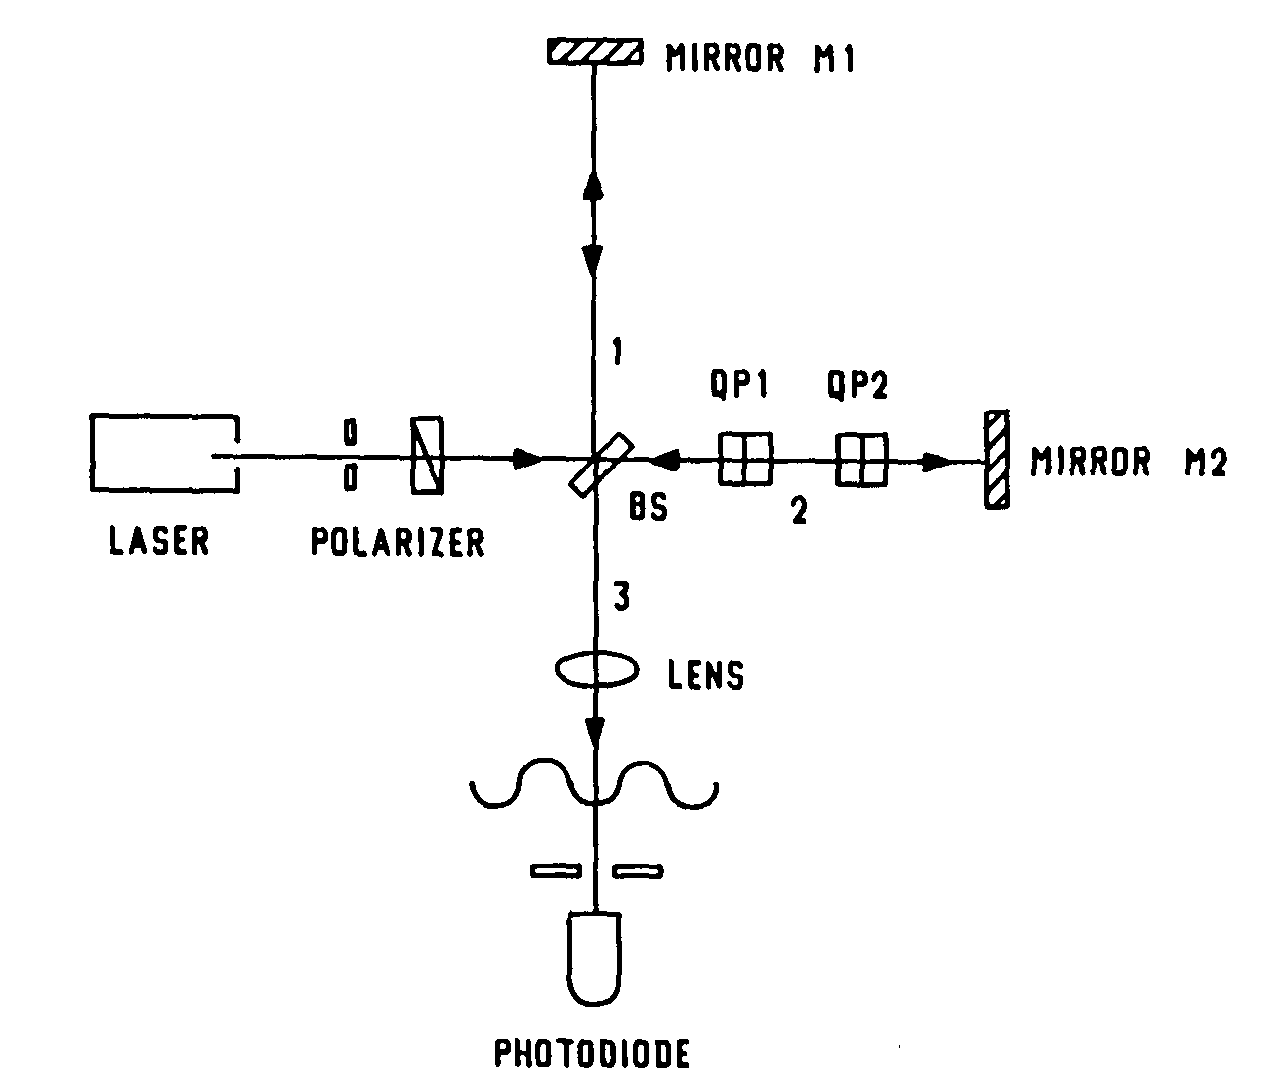
\includegraphics[width=6.5cm]{pb expt.png}
	\caption{Schematic of Michelson interferometer setup for observation of Pancharatnam-Berry phase (ref. \cite{chyba 88})}
	\label{fig:pb expt}
\end{figure}

 Fast axis of QP1 and QP2 are aligned at $\theta_1= \pi/4$ and $\theta_2= \beta$ \textit{w.r.t.} x-axis, respectively. The input light is x-polarized. Then the polarization state of output light at different part of arm 2 in Michelson interferometer is shown in fig \ref{fig:pancha}, and corresponding Jones calculus shown in table \ref{table:5}.
 

\begin{table}[H]
 	\centering
 	\begin{tabular}{c c} 
	\hline
	\hline
	\begin{tabular}{c}
		Poincare  \\
		Sphere point \\
		(pol. state) 
	\end{tabular}&
	\begin{tabular}{c}
		Polarization state\\
		(Jones vector, $\boldsymbol{J}$)
	\end{tabular} \\\hline
 	
 	 A $(\ket{A})$ & $\boldsymbol{J}_A= \begin{bmatrix}1 \\ 0\end{bmatrix}$\\\hline
 	
 	 R $(\ket{R})$ & 
 	 \parbox{5cm}{\begin{align*}
 	 	\boldsymbol{J}_R 
 	 	&= R(-\pi/4)\:\boldsymbol{M}_{QP}\:R(\pi/4) \;\boldsymbol{J}_A = \frac{e^{i\phi'}}{2}\begin{bmatrix}1+i&1-i \\ 1-i & 1+i\end{bmatrix} \begin{bmatrix}1 \\ 0\end{bmatrix}\\
 	 	&= \frac{e^{i\phi'}}{2}\begin{bmatrix}1+i\\1-i\end{bmatrix} = \frac{1}{\sqrt{2}}\begin{bmatrix}1\\-i\end{bmatrix} \exp(i\phi_1)
 	 \end{align*}}\\\hline
 	
 	 B $(\ket{B})$& 
 	\parbox{5cm}{\begin{align*}
 			\boldsymbol{J}_B 
 			&=R(-\beta)\:\boldsymbol{M}_{QP}\:R(\beta) \;\boldsymbol{J}_R\\
 			&= e^{i\phi''}
 			\begin{bmatrix}
 				\cos[2](\beta)+i\sin[2](\beta)&(1-i)\sin(\beta)\cos(\beta) \\ 
 				(1-i)\sin(\beta)\cos(\beta) & \sin[2](\beta)+i\cos[2](\beta)
 			\end{bmatrix} 
 		\frac{1}{\sqrt{2}}\begin{bmatrix}1 \\ -i\end{bmatrix}\exp(i\phi_1)\\
 			&=\begin{bmatrix}\cos(\beta+\pi/4)\\\sin(\beta+\pi/4)\end{bmatrix} \exp(i\phi_2)\:\exp(-i\beta)\\
 			& = \begin{bmatrix}\cos(\varphi)\\\sin(\varphi)\end{bmatrix} \exp(i\phi_3)\:{\color{red}\exp(-i\varphi)}\:\text{ where }\:\varphi= \beta+\pi/4
 	\end{align*}}\\\hline
 	
 	C $(\ket{C})$&
 	\parbox{5cm}{\begin{align*}
 			\boldsymbol{J}_C 
 			&=\boldsymbol{M}_{Mirror} \;\boldsymbol{J}_B
 			= e^{i\pi}
 			\begin{bmatrix}
 				-1 & 0 \\ 0 & 1
 			\end{bmatrix} 
 			\begin{bmatrix}\cos(\varphi)\\\sin(\varphi)\end{bmatrix} \exp(i\phi_3)\:{\color{red}\exp(-i\varphi)}\\
 			&=\begin{bmatrix}-\cos(\varphi)\\\sin(\varphi)\end{bmatrix} \exp(i\phi_4)\:{\color{red}\exp(-i\varphi)}
 	\end{align*}}\\\hline
 	
 	L $(\ket{L})$&
 	\parbox{5cm}{\begin{align*}
 			\boldsymbol{J}_L 
 			=\begin{bmatrix}1\\i\end{bmatrix} \exp(i\phi_5)\:{\color{red}\exp(-i\:2\varphi)}
 	\end{align*}}\\\hline
 
 	A $(\ket{A'})$&
 	\parbox{5cm}{\begin{align*}
 			\boldsymbol{J}_A' 
 			&=\begin{bmatrix}1\\0\end{bmatrix} \exp(i\phi_6)\:{\color{red}\exp(-i\:2\varphi)}\\
 			&=\boldsymbol{J}_A \exp(i\phi_6)\:{\color{red}\exp(-i\:2\varphi)}
 	\end{align*}}\\
 	\hline
 	\hline
	\end{tabular}
 	\caption{Jones vector of polarization state in Pancharatnam-Berry phase}
 	\label{table:5}
\end{table}

 \begin{figure}[t]
	\begin{subfigure}[H]{0.50\textwidth}
		\centering
		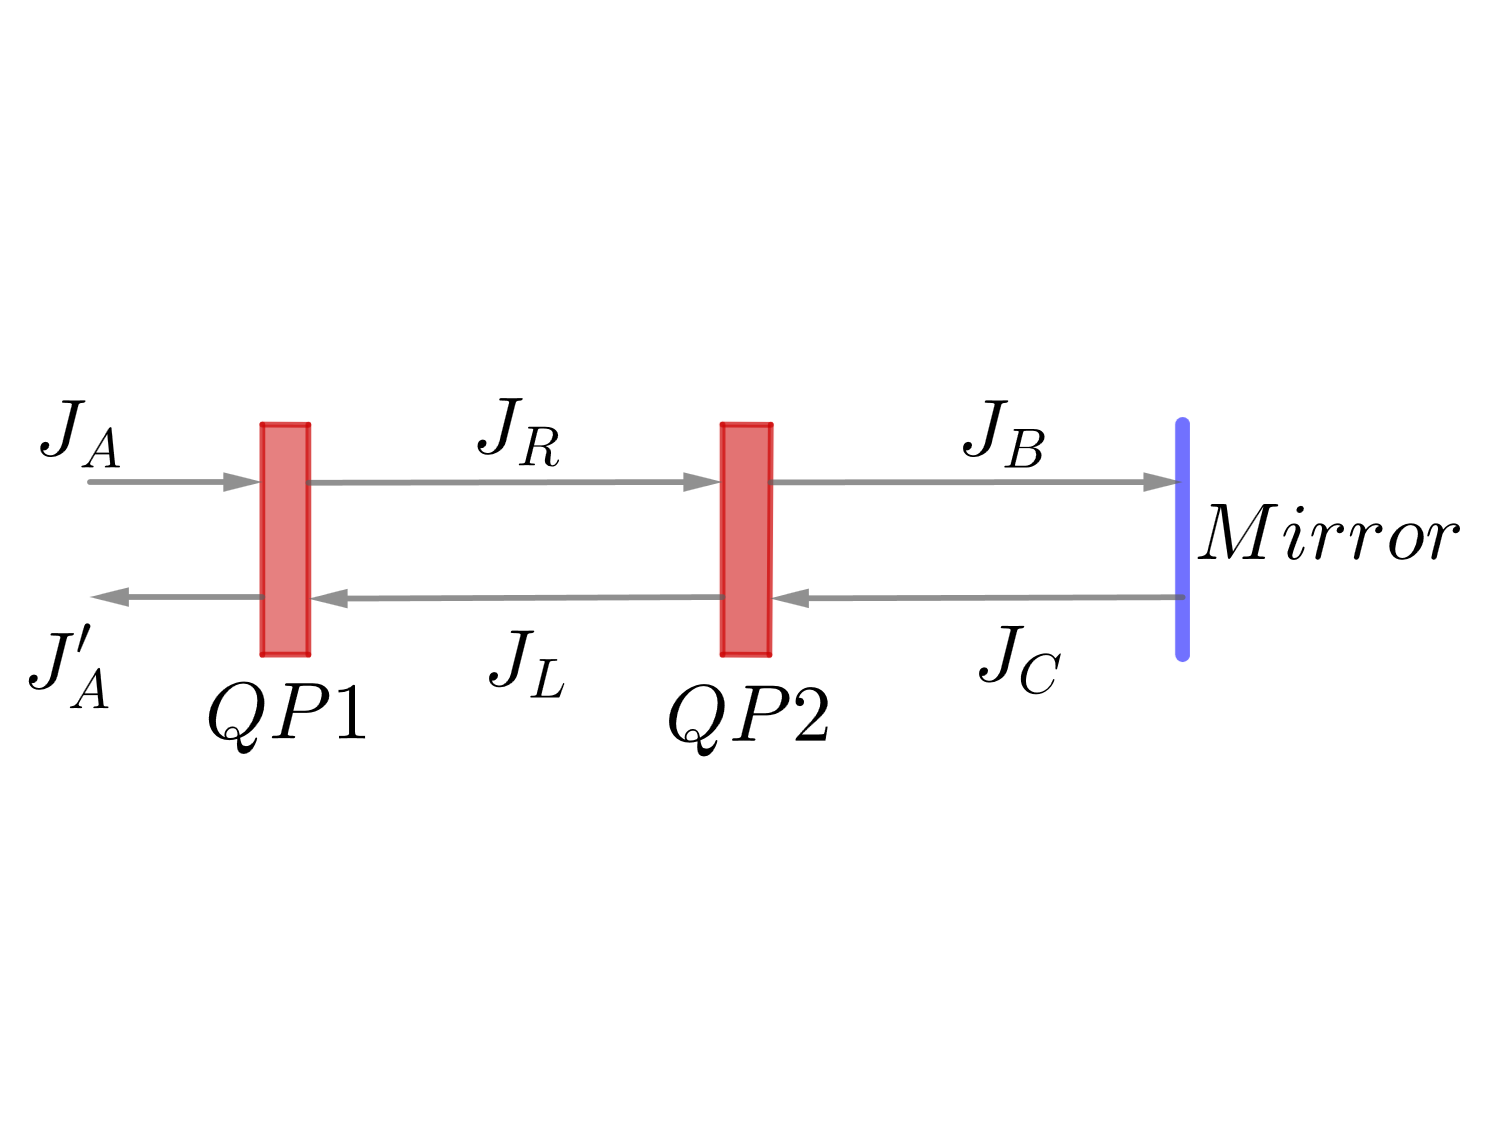
\includegraphics[width=0.9\textwidth]{MI arm.png}
		\caption{Michelson interferometer arm 2}
		\label{fig:pancha a}
	\end{subfigure}
	\hfil
	\begin{subfigure}[H]{0.4\textwidth}
		\centering
		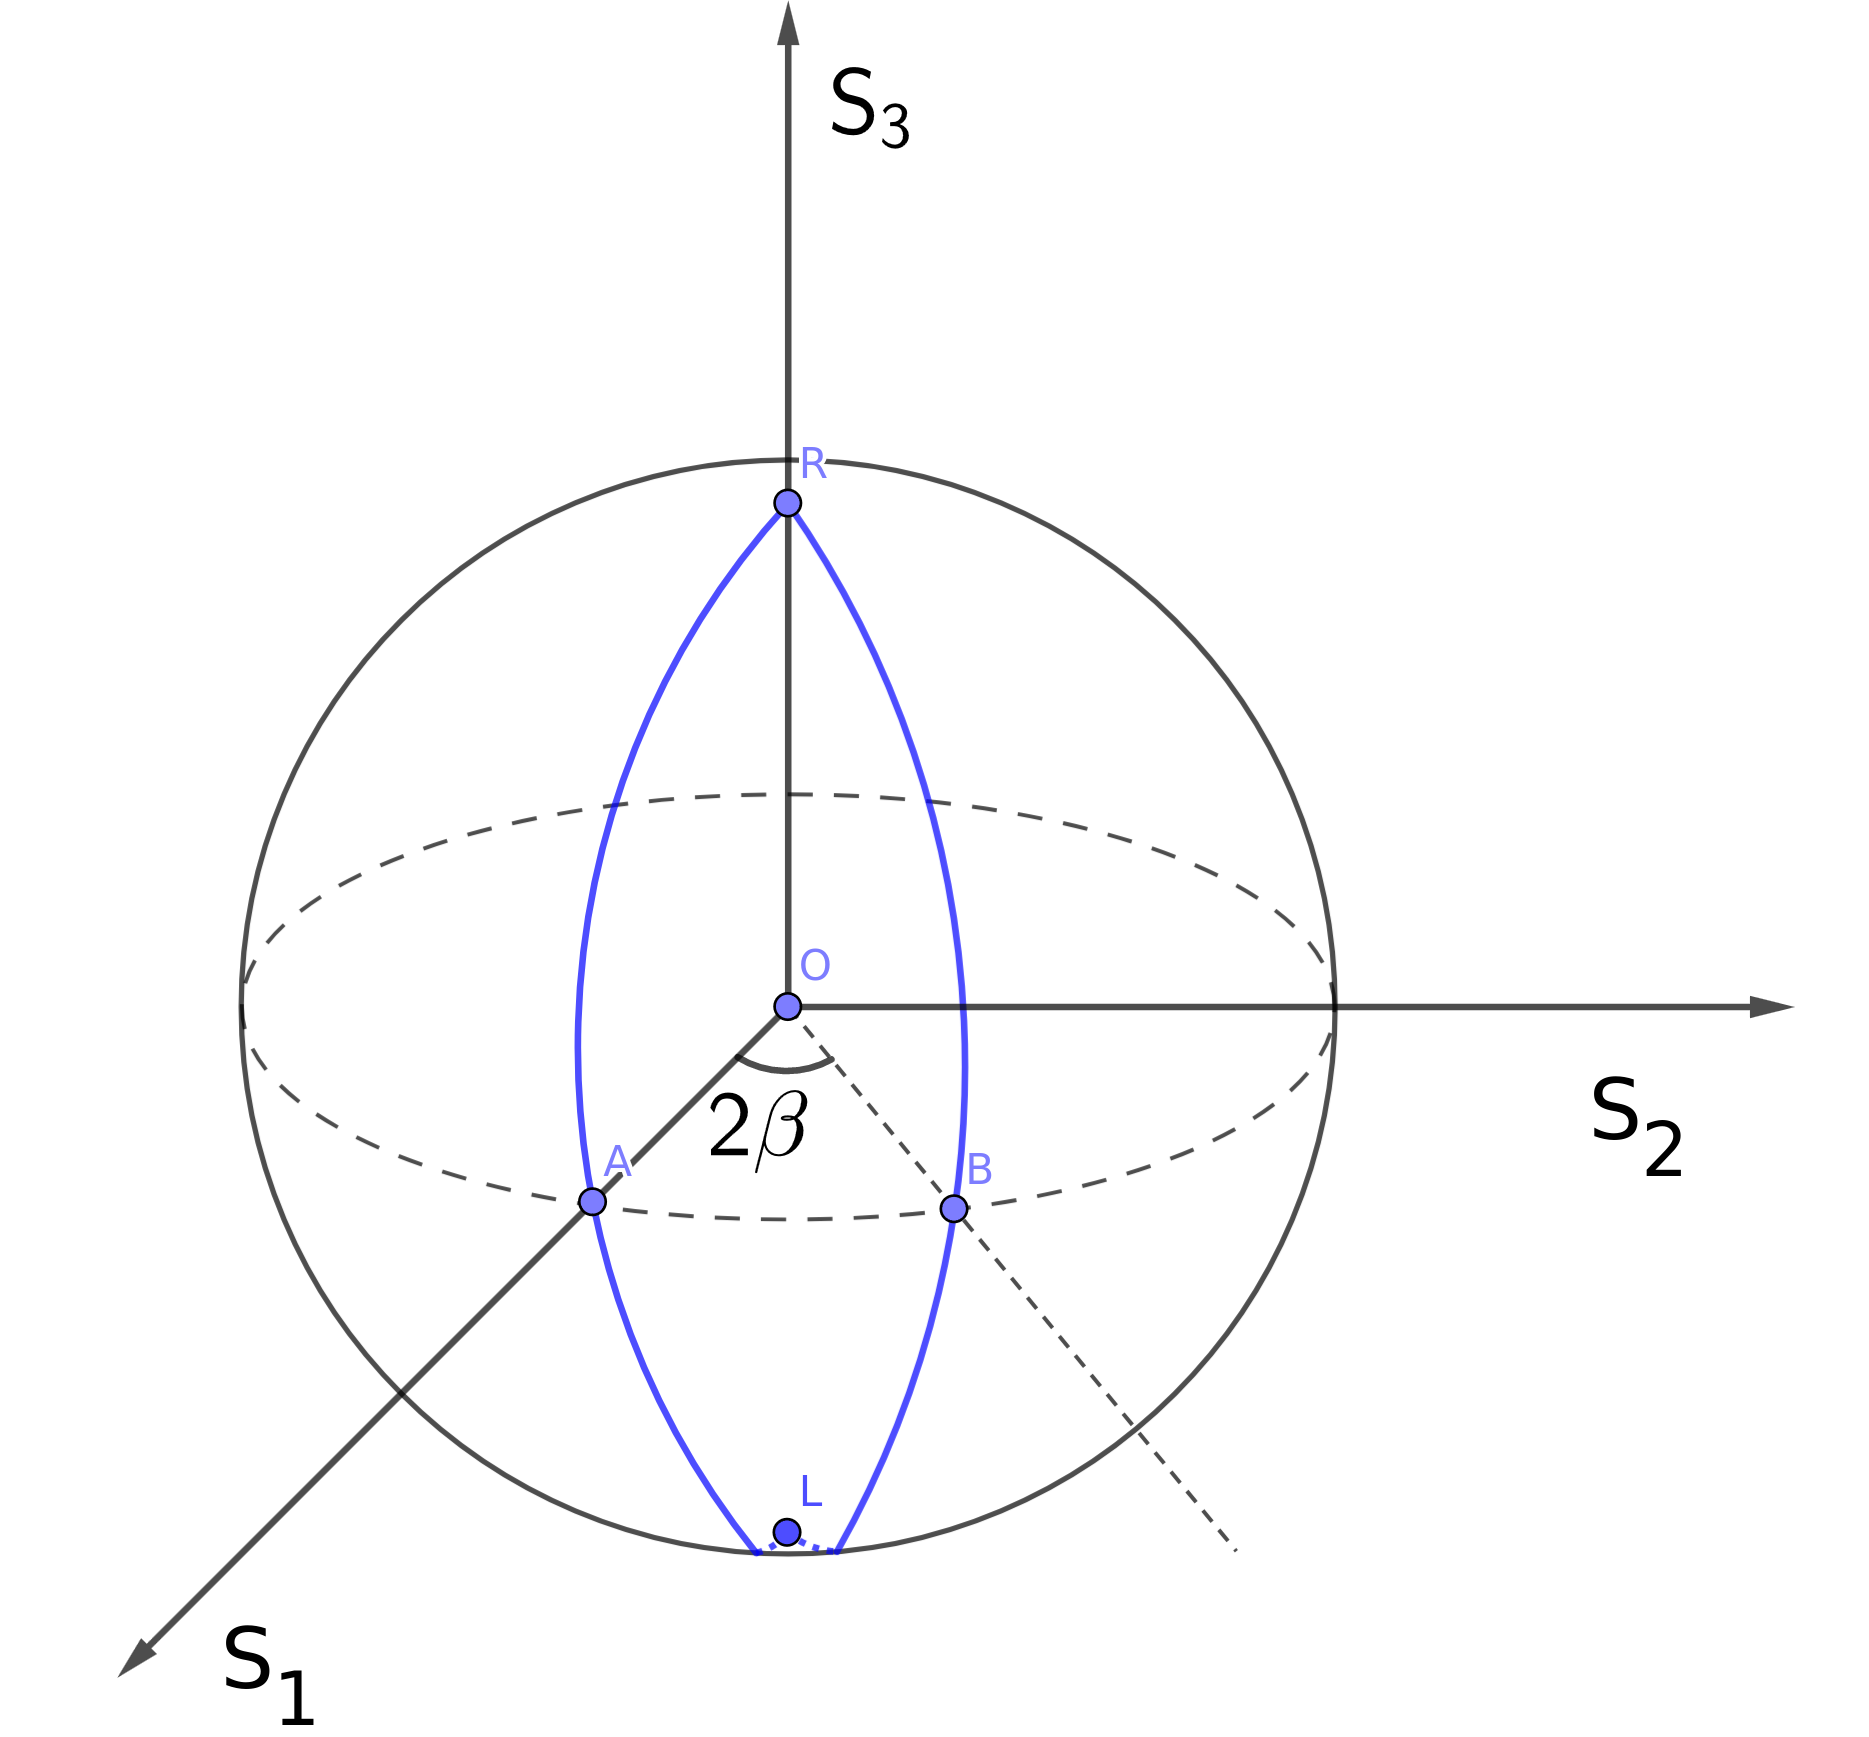
\includegraphics[width=0.9\textwidth]{poincare-pb.png}
		\caption{Corresponding cyclic evolution in Poincare sphere}
		\label{fig:pancha b}
	\end{subfigure}
	\caption{Evolution of polarization state in arm 2}
	\label{fig:pancha}
\end{figure}


We see that the light with linear polarization state $(\ket{B})$ acquired a additional phase term \textit{i.e.} ${\color{red}\exp(-i\:2\varphi)}$ which only depends on orientation of QP2 \textit{i.e.} $\varphi= \beta+\pi/4$ and does not depend on thickness and refractive index of the birefringent wave-plate, so this phase is purely geometric one. Other all $\phi$'s are all dynamical phase factors. \cite{WO}

We see after one cyclic evolution in Poincare sphere in path ARBCLA,
\begin{align}
	\ket{A}\longrightarrow\ket{A'}=\ket{A}\exp(i\phi_6-i\:2\varphi)
\end{align}

So at photodiode the intensity variation \textit{w.r.t.} $\beta$ will be
\begin{align}
	I &= (\bra{A}+\bra{A'})(\ket{A}+\ket{A'}) \nonumber\\
	&= \braket{A}{A} \left(1+\exp(-i\phi_6+i2\varphi)\right)\left(1+\exp(i\phi_6-i2\varphi)\right)\nonumber\\
	&= \braket{A}{A}(2 + 2\cos(2\varphi - \phi_6))\nonumber\\
	\Rightarrow I(\beta)&= 2\braket{A}{A} \left(1- \sin(2\beta - \phi_6)\right) \label{eq:4.16}
\end{align}
Experimental verification by Chyba \textit{et al} (ref. \cite{chyba 88}) is given in figure \ref{fig:chyba}.
\begin{figure}[H]
	\begin{subfigure}[H]{0.53\textwidth}
		\centering
		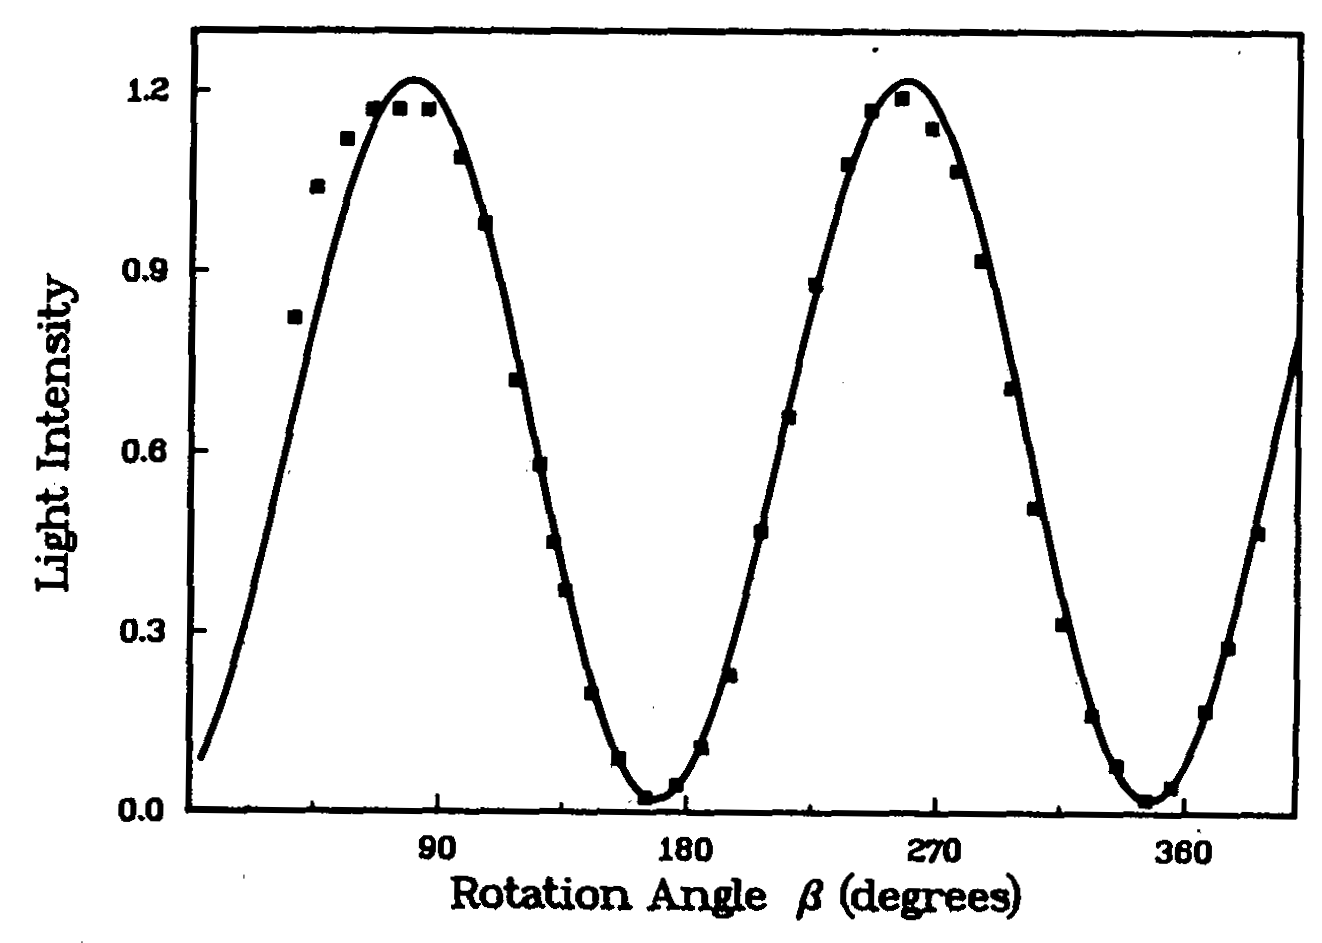
\includegraphics[width=0.9\textwidth]{chyba 1.png}
		\caption{Measured intensity vs Rotation angle  $\beta$ of QP2, fitted with eq. \ref{eq:4.16} }
		\label{fig:chyba a}
	\end{subfigure}
	\hfil
	\begin{subfigure}[H]{0.41\textwidth}
		\centering
		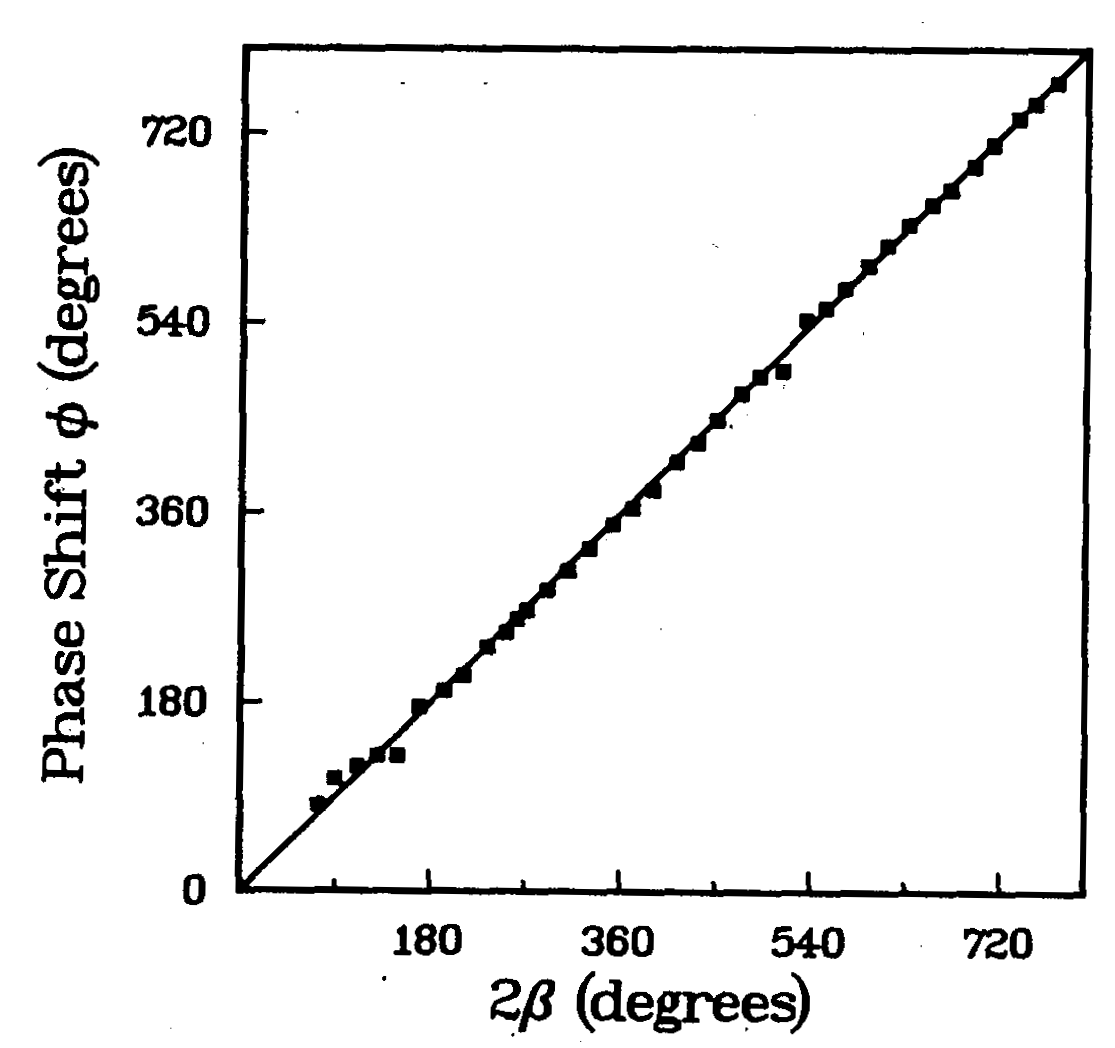
\includegraphics[width=0.9\textwidth]{chyba 2.png}
		\caption{Measured phase shift vs rotation angle $\beta$, with solid line of $\phi=2\beta$}
		\label{fig:chyba b}
	\end{subfigure}
	\caption{Measurement of the Pancharatnam phase by Chyba \textit{et al} (ref. \cite{chyba 88})}
	\label{fig:chyba}
\end{figure}


\subsubsection{Rotational frequency shift of light}
Rotational frequency shift is the dynamical manifestation of Pancharatnam-Berry Phase. Let there is half wave-plate rotating \textit{w.r.t.} centre axis at $\Omega$. If the alignment of the fast axis of half wave-plate is $\theta$, then
\begin{align}
	\Omega = \frac{d\theta}{dt}\\
	\theta = \Omega t
\end{align}

let the Jones electric field vector of input light is
 \begin{align}
 	\boldsymbol{E}_{in} = \frac{1}{\sqrt{2}}
 	\begin{bmatrix}
 		1\\i\sigma
 	\end{bmatrix}
 \end{align}
Then the Jones electric field vector of output light is
\begin{align}
	\boldsymbol{E}_{out}(\theta)&=R(-\theta)\boldsymbol{M}_{\lambda/2}R(\theta)\boldsymbol{E}_{in}
	=R(-\theta)
	\begin{bmatrix}
		1 & 0\\
		0 & -1
	\end{bmatrix}
	R(\theta)\boldsymbol{E}_{in}\nonumber\\
	&=\begin{bmatrix}
		\cos(2\theta) & \sin(2\theta)\\
		\sin(2\theta) & -\cos(2\theta)
	\end{bmatrix}
	\frac{1}{\sqrt{2}}
	\begin{bmatrix}
		1\\i\sigma
	\end{bmatrix}
	= \frac{1}{\sqrt{2}}
	\begin{bmatrix}
		1\\-i\sigma
	\end{bmatrix}
	{\color{blue}\exp(i2\sigma\theta)}\nonumber\\
	\Rightarrow\boldsymbol{E}_{out}(t)&= \frac{1}{\sqrt{2}}
	\begin{bmatrix}
		1\\-i\sigma
	\end{bmatrix}
	{\color{blue}\exp(i2\sigma\Omega t)}
\end{align}
If angular frequency of the input beam is $\omega$, then the angular frequency of output beam be $(\omega + 2\sigma\Omega)$. So change in angular frequency, $\Delta\omega=2\sigma\Omega$. This is spin-dependant \textit{rotational Doppler shift} of SAM carrying light beam. \cite{WO}

%\subsubsection{\color{red}Geometric phase in LG-HG mode transformation}

\subsection{Types of SOI}
We have discussed brief of angular momentum of light in previous chapter. The different types of angular momentum a EM beam carries are
\begin{enumerate}
	\item Spin AM ($\boldsymbol{S}$) or SAM
	\item Intrinsic orbital AM ($\boldsymbol{L}_{int}$) or IOAM
	\item Extrinsic orbital AM ($\boldsymbol{L}_{ext}$) or EOAM
\end{enumerate}
SAM is associated with degree of circular polarization and also intrinsic in nature. The IOAM is associated with the optical vortex structure of the beam (\textit{e.g.} vortex beam like LG beam), so it is intrinsic. Whereas the EOAM is associated with the trajectory of centroid of the beam. \cite{bliokh 12} (see fig \ref{fig:am}) 
\begin{figure}[H]
	\begin{subfigure}[H]{0.32\textwidth}
		\centering
		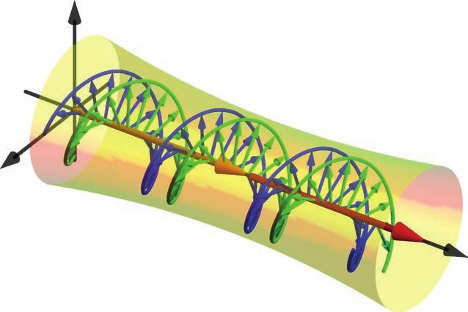
\includegraphics[width=0.95\textwidth]{sam.png}
		\caption{SAM of RCP beam of $\sigma=-1$}
		\label{fig:sam}
	\end{subfigure}
	\hfil
	\begin{subfigure}[H]{0.31\textwidth}
		\centering
		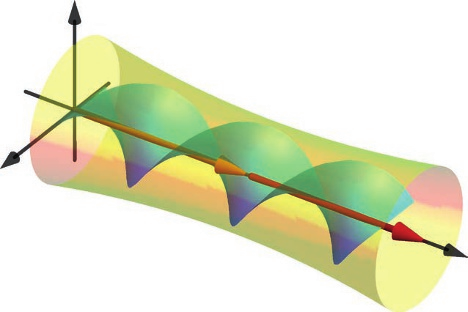
\includegraphics[width=0.95\textwidth]{ioam.png}
		\caption{Intrinsic OAM of vortex beam of $l=2$}
		\label{fig:ioam}
	\end{subfigure}
	\hfil
	\begin{subfigure}[H]{0.31\textwidth}
		\centering
		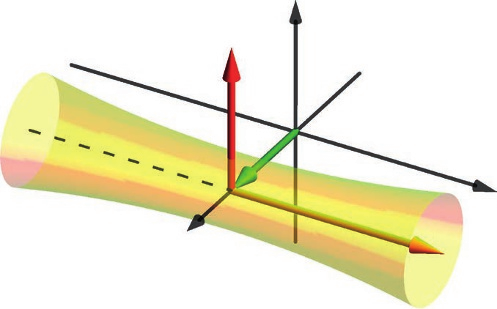
\includegraphics[width=0.95\textwidth]{eoam.png}
		\caption{Extrinsic OAM of beam at $\boldsymbol{R}$ away from origin}
		\label{fig:eoam}
	\end{subfigure}
	\caption{Angular momentum of paraxial beam (ref. \cite{bliokh 15})}
	\label{fig:am}
\end{figure}

The inter-conversion between these different angular momentum in a process represents \textit{spin-orbit interaction} of light. \cite{bliokh 15} The three type of interaction  are
\begin{enumerate}
	\item between $\boldsymbol{S}$ and $\boldsymbol{L}_{int}$
	\item between $\boldsymbol{S}$ and $\boldsymbol{L}_{ext}$
	\item between $\boldsymbol{L}_{int}$ and $\boldsymbol{L}_{ext}$
\end{enumerate}
In the later section, we will see several manifestation of those interactions.

%\subsection{SOI in isotropic medium}
%\cite{bliokh 12}

\subsection{SOI in anisotropic medium}
Inhomogeneous anisotropic medium has spatially varying anisotropy axis (\textit{i.e.} birefringent or dichroic. Here SOI deals with spin flipping, spin-to-orbital angular momentum conversion etc. To illustrate these events, we will consider specific cases.

A simple case of homogenous medium is when a circularly polarized light passes through quarter wave-plate, it become linearly polarized light, so the SAM transformation is $$\sigma=\pm1 \longrightarrow \sigma= 0$$ 
In that case, $\pm\hbar$ SAM carried by each photon of circularly polarized light, is transferred to the wave plate. Similarly for half wave-plate, the SAM transformation is 
$$\sigma=\pm 1 \longrightarrow \sigma=\mp1$$ So the spin is flipped.

Before going into more complex cases, we discuss about \textit{q-plate}. Q-plate is an birefringent anisotropic media of specific phase retardation across the slab with an inhomogeneous orientation of the fast (or slow) optical axis lying parallel to the slab planes whose local alignment of birefringent fast axis varies linearly with the azimuth angle of the q-plate. \cite{marrucci 06} Let local alignment angle is $\alpha$, and the azimuth angle is $\phi$, then,
\begin{align}
	\alpha(\phi)=q\phi+\alpha_0
\end{align}
\begin{figure}[H]
\centering
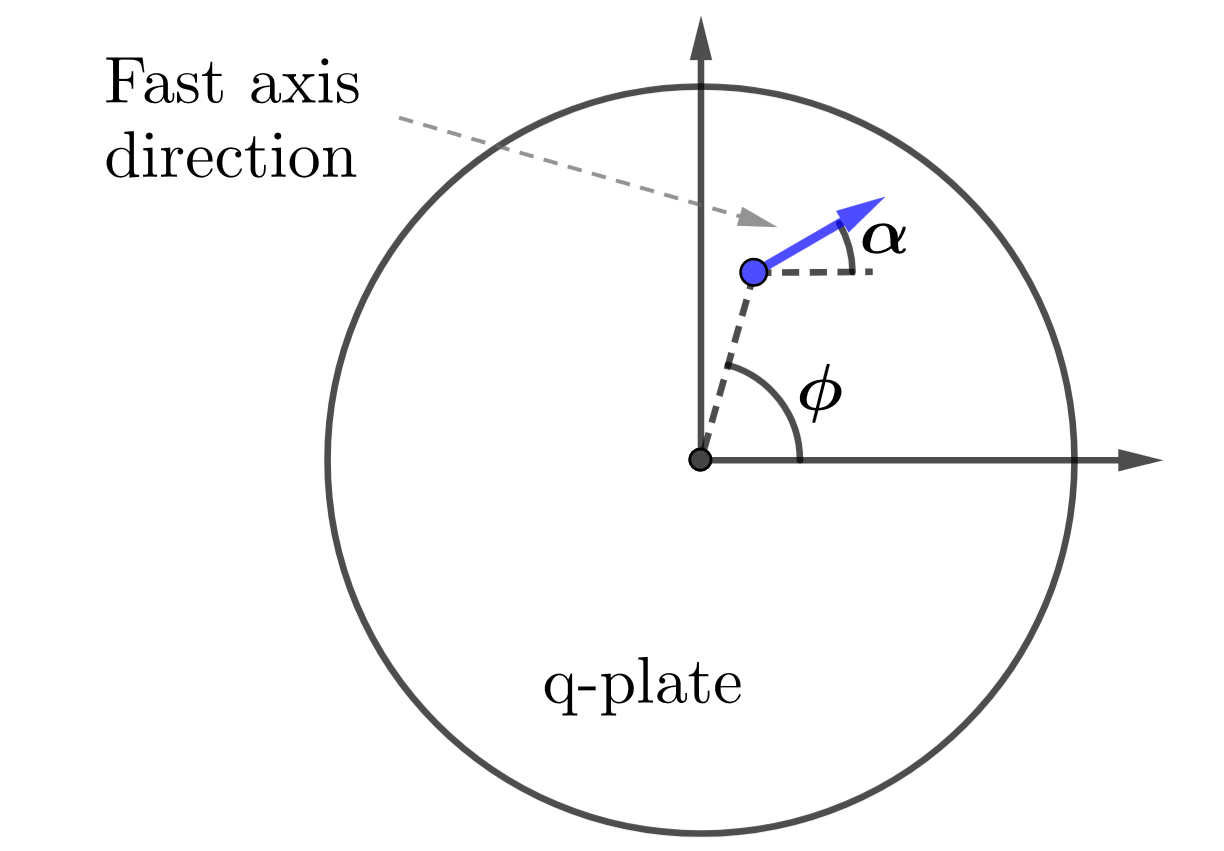
\includegraphics[width=0.4\linewidth]{q-plate}
\caption{local birefringent fast axis alignment in q-plate}
\label{fig:q-plate}
\end{figure}

Now the corresponding Jones matrix at each point of the q-plate of phase retardation of $\pi$, will be \cite{marrucci 06}
\begin{align}
	\boldsymbol{M}_q(\phi)&=R(-\alpha)\boldsymbol{M}_{\lambda/2}R(\alpha) 
	=R(-\alpha)
	\begin{bmatrix}
		1 & 0\\
		0 & -1
	\end{bmatrix}
	R(\alpha)\nonumber\\
	 &=\begin{bmatrix}
		\cos(2\alpha) & \sin(2\alpha)\\
		\sin(2\alpha) & -\cos(2\alpha)
	\end{bmatrix}
\end{align}

Let considering transversal of electric field, for each ray of a paraxial beam of circular polarization ($\sigma=\pm1$) the Jones electric field is 
\begin{align}
	\boldsymbol{E}_{in} = \frac{1}{\sqrt{2}}
	\begin{bmatrix}
		1\\i\sigma
	\end{bmatrix}
\end{align}
then the output electric filed vector will be
\begin{align}
	\boldsymbol{E}_{out}(\phi) = \boldsymbol{M}_q(\phi)
	\frac{1}{\sqrt{2}}
	\begin{bmatrix}
		1\\i\sigma
	\end{bmatrix}
	= \exp(i2\sigma\alpha)\frac{1}{\sqrt{2}}
	\begin{bmatrix}
		1\\-i\sigma
	\end{bmatrix}
	=\frac{1}{\sqrt{2}}
	\begin{bmatrix}
		1\\-i\sigma
	\end{bmatrix}
	{\color{red}\exp(i2\sigma q\phi)}\: \exp(i2\sigma\alpha_0)
\end{align}
So the output beam has spin flipping. Moreover the beam has acquired a spin-dependant phase factor  ${\color{red}\exp(i2\sigma q\phi)}$, which makes it a vortex beam. From \ref{eq:3.32} we see that output light carries $2q\hbar$ angular momentum per photon. Here the change of angular momentum is 
$$(\sigma=\pm1,l=0)\longrightarrow (\sigma=\mp1,l=\pm2q)$$
So to keep total angular momentum per photon conserved, $q=1$.


Now let the q-plate is of phase retardation of $\pi/2$, then 
\begin{align}
	\boldsymbol{M}_q(\phi)&=R(-\alpha)\boldsymbol{M}_{\lambda/4}R(\alpha) 
	=R(-\alpha)
	\begin{bmatrix}
		1 & 0\\
		0 & i
	\end{bmatrix}
	R(\alpha)\nonumber\\
	&=\begin{bmatrix}
		\cos[2](\alpha)+i\sin[2](\alpha)&(1-i)\sin(\alpha)\cos(\alpha) \\ 
		(1-i)\sin(\alpha)\cos(\alpha) & \sin[2](\alpha)+i\cos[2](\alpha)
	\end{bmatrix}
\end{align}
Putting circularly polarized light (as in Pancharatnam-Berry phase, see table \ref{table:5}), electric filed vector will be
\begin{align}
	\boldsymbol{E}_{out}(\phi) &= \boldsymbol{M}_q(\phi)\frac{1}{\sqrt{2}}
	\begin{bmatrix}
		1\\
		i\sigma
	\end{bmatrix}
	= \exp(i\sigma\alpha)
	\begin{bmatrix}
		\cos(\alpha - \sigma\pi/4)\\
		\sin(\alpha - \sigma\pi/4)
	\end{bmatrix}\nonumber\\
	&=\begin{bmatrix}
		\cos(\alpha - \sigma\pi/4)\\
		\sin(\alpha - \sigma\pi/4)
	\end{bmatrix}
	{\color{red}\exp(i\sigma q\phi)}\:\exp(i\sigma\alpha_0)
\end{align}
So the output beam has a phase factor ${\color{red}\exp(i\sigma q\phi)}$. Here the change of angular momentum is 
$$(\sigma=\pm1,l=0)\longrightarrow (\sigma=0,l=\pm q)$$
So to keep total angular momentum per photon conserved, $q=1$.

\begin{figure}[H]
	\begin{subfigure}[H]{0.24\textwidth}
		\centering
		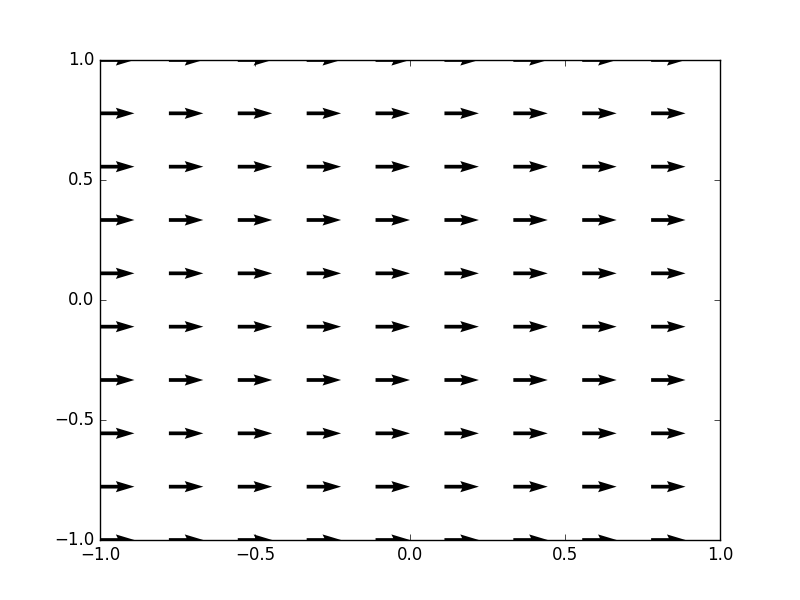
\includegraphics[width=\textwidth]{qplate(0).png}
		\caption{$q=0$, $\alpha_0=0$}
		\label{fig:q0}
	\end{subfigure}
	\hfil
	\begin{subfigure}[H]{0.24\textwidth}
		\centering
		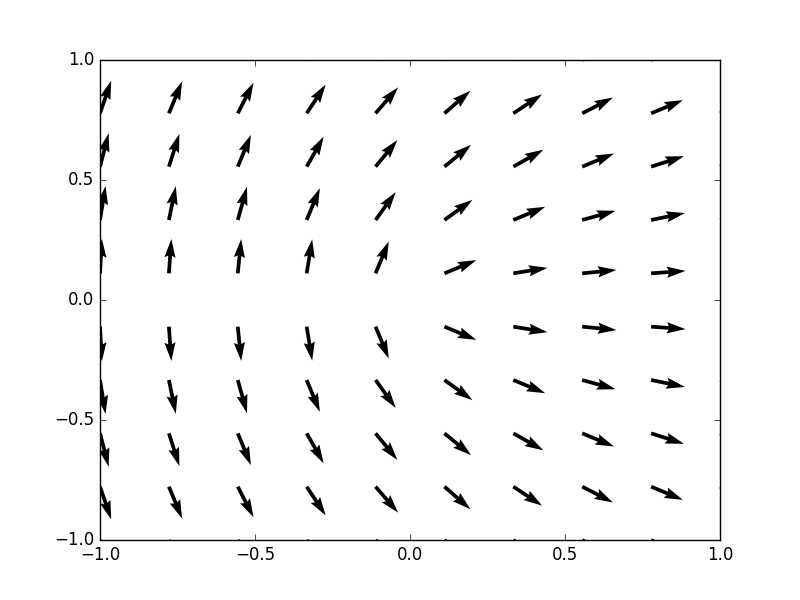
\includegraphics[width=\textwidth]{qplate(0.5).png}
		\caption{$q=0.5$, $\alpha_0=0$}
		\label{fig:q0.5}
	\end{subfigure}
	\hfil
	\begin{subfigure}[H]{0.24\textwidth}
		\centering
		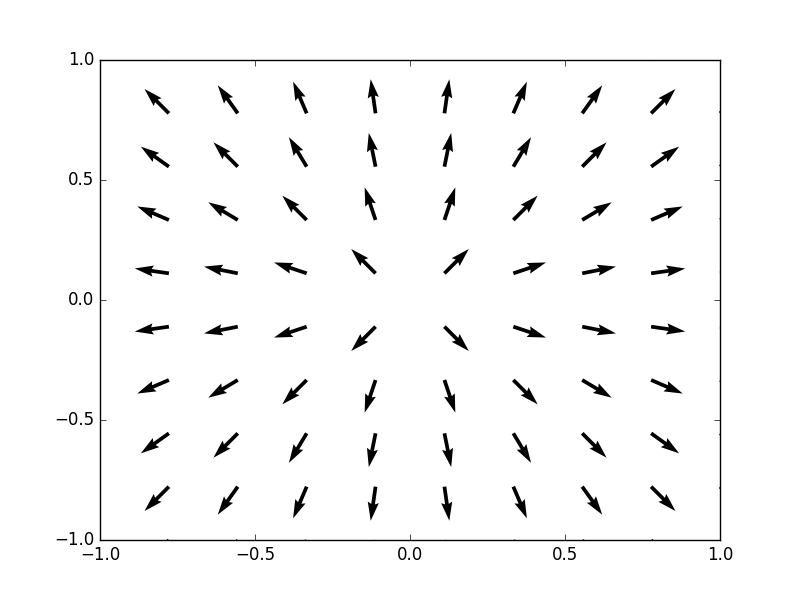
\includegraphics[width=\textwidth]{qplate(1).png}
		\caption{$q=1$, $\alpha_0=0$}
		\label{fig:q1}
	\end{subfigure}
	\hfil
	\begin{subfigure}[H]{0.24\textwidth}
		\centering
		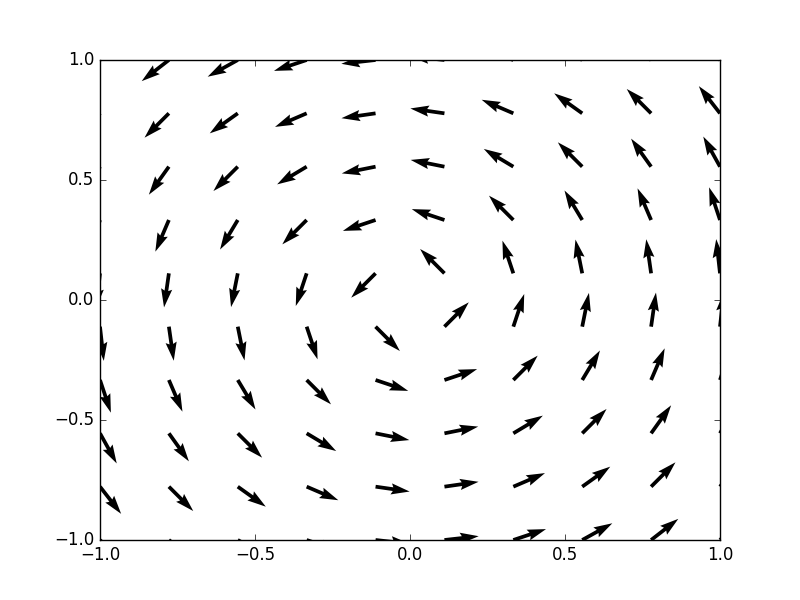
\includegraphics[width=\textwidth]{qplate(1,r).png}
		\caption{$q=1$, $\alpha_0=\pi/2$}
		\label{fig:q1r}
	\end{subfigure}
	\caption{Q-plate of different $q$ and $\alpha_0$}
	\label{fig:qplate}
\end{figure}


\cite{beijer 94}
\cite{yao 11} pg - 168
Another Inhomogeneous medium is spiral phase plate (see fig \cite{beijer 94}).




%\subsection{SOI in non-paraxial fields}
%\subsection{Spin Hall effect}


\clearpage
\let\oldbibliography\thebibliography
\renewcommand{\thebibliography}[1]{%
	\oldbibliography{#1}%
	\setlength{\itemsep}{0pt}%
}
\pagenumbering{roman}
\small
\fontfamily{lmtt}\selectfont

\begin{thebibliography}{999}
	\bibitem{WO}
	Gupta, S.D., Ghosh, N., \& Banerjee, A. (2015). Wave Optics: Basic Concepts and Contemporary Trends (1st ed.). CRC Press. doi:10.1201/b19330
	
	\bibitem{born-wolf}
	Born, Max; Wolf, Emil (1999). Principles of optics: electromagnetic theory of propagation, interference and diffraction of light (7th expanded ed.). Cambridge: Cambridge University Press. ISBN 0-521-64222-1. OCLC 1151058062
	
	\bibitem{jones}
	\href{https://en.wikipedia.org/wiki/Jones_calculus}{Jones Calculus - Wikipedia}
	
	\bibitem{coherency}
	Wang Jizhong (1986). A matrix method for describing unpolarized light and its applications. , 2(4), 362–372. doi:10.1007/bf02488478
	
	\bibitem{yt video}
	\href{https://www.youtube.com/watch?v=RowMxWt4mVE&list=LL&index=5}{Polarization (Jones vectors and matrices, partial polarization, Stokes parameters)}
	
	\bibitem{stokes}
	Hecht, Eugene (1970). Note on an Operational Definition of the Stokes Parameters. American Journal of Physics, 38(9), 1156–. doi:10.1119/1.1976574    
	
	\bibitem{milonni}
	Milonni, P.W. and Eberly, J.H. (2010). Laser Physics. Wiley \& Sons, Hoboken, Chapter 7. doi: 10.1002/9780470409718
	
	\bibitem{cornell}
	\href{https://www.youtube.com/playlist?list=PLyWzPf87clvEb8T3Xf30tMaUqdbVchrNY}{Lasers and Optoelectronics: ECE 4300 Cornell University} 
	
	\bibitem{kogelnik 66}
	Kogelnik, H., \& Li, T. (1966). Laser beams and resonators. Applied optics, 5(10), 1550-1567. 
	
	\bibitem{opt cavity}
	\href{https://en.wikipedia.org/wiki/Optical_cavity}{Optical cavity - Wikipedia}
	
	\bibitem{erikson 94}
	Erikson, W. L.; Singh, S. (1994). Polarization properties of Maxwell-Gaussian laser beams. Physical Review E, 49(6), 5778–5786. doi: 10.1103/PhysRevE.49.5778
	
	\bibitem{max eq - wiki}
	\href{https://en.wikipedia.org/wiki/Maxwell's_equations}{Maxwell's equations - Wikipedia}
	
	%\bibitem{hall 96}
	%Hall, Dennis G. (1996). Vector-beam solutions of Maxwell’s wave equation. ol/21/1/ol-21-1-9.pdf, 21(1), 9–0. doi:10.1364/OL.21.000009  
	
	\bibitem{conry 12}
	Conry, J. P. (2012). Polarization Properties of Maxwell-Gauss Laser Beams. Graduate Theses and Dissertations Retrieved from \href{https://scholarworks.uark.edu/etd/491}{https://scholarworks.uark.edu/etd/491}.
	
	\bibitem{lewis 14}
	 Lewis, W. E.; Vyas, R. (2014). Maxwell-Gaussian beams with cylindrical polarization. Journal of the Optical Society of America A, 31(7), 1595–. doi: 10.1364/josaa.31.001595 
	
	\bibitem{n dist}
	\href{https://en.wikipedia.org/wiki/Normal_distribution}{Normal distribution - Wikipedia}
	
	\bibitem{LG}
	\href{https://flex.phys.tohoku.ac.jp/~rsaito/saito20-GaussianBeam.pdf}{Introduction of Gaussian Beam - Tohoku University}
	
	\bibitem{babiker 12}
	Andrews, D., \& Babiker, M. (Eds.). (2012). The Angular Momentum of Light. Cambridge: Cambridge University Press. doi: 10.1017/CBO9780511795213
	
	
	\bibitem{beijers allen 93}
	MW Beijersbergen, L Allen, H Van der Veen, and JP Woerdman (1993). Astigmatic laser mode converters and transfer of orbital angular momentum. Opt. Commun., 96(1):123–132.
	
	\bibitem{enk nien 92}
	 S.J. van Enk; G. Nienhuis (1992). Eigenfunction description of laser beams and orbital angular momentum of light. 94(1-3), 147–158. doi: 10.1016/0030-4018(92)90424-p     
	 
	 \bibitem{allen 99}
	 Allen, L. (1999).The Orbital Angular Momentum of Light. Progress in Optics.  Volume 39. 291–372. doi: 10.1016/S0079-6638(08)70391-3
	 
	 \bibitem{levedev}
	 Lebedev, N. N. (1972), Special Functions and Their Applications, Dover Publications Inc.
	 
	 \bibitem{abra 91}
	 Abramochkin, E. and Volostnikov, V. (1991) Beam Transformations and Nontransformed Beams. Optics Communications, 83, 123-135. 
	 
	 \bibitem{poynting}
	 \href{https://en.wikipedia.org/wiki/Poynting_vector}{Poynting vector - Wikipedia}
	  
	 \bibitem{haus}
	 Haus, Hermann A. (1984). Waves and fields in optoelectronics. Englewood Cliffs, NJ :Prentice-Hall.
	 
	 \bibitem{bernatt allen 94}
	 Barnett, S. \& Allen, L. (2010). Orbital angular momentum and nonparaxial light beams. Opt. Commun. 110. 670-678. doi: 10.1016/0030-4018(94)90269-0.
	 
	 \bibitem{CCT} 
	 Cohen-Tannoudji, C., J. Dupont-Roc, and G. Grynberg (1989), Photons and. Atoms, Introduction to Quantum Electrodynamics, John Wiley \& Sons,. New York.
	 
	 \bibitem{melvin 75}
	 Lax, Melvin; Louisell, William H.; McKnight, William B. (1975). From Maxwell to paraxial wave optics. Physical Review A, 11(4), 1365–1370. doi: 10.1103/PhysRevA.11.1365
	 
	 \bibitem{berry 98}
	  Berry, Michael V.; Soskin, Marat S. (1998). SPIE Proceedings., International Conference on Singular Optics - Paraxial beams of spinning light., 3487(), 6–11. doi: 10.1117/12.317704 
	  
	  \bibitem{zettili 09}
	  Zettili N. (2009). Quantum mechanics : concepts and applications (2nd ed.). Wiley.
	  
	  \bibitem{relativity -wiki}
	  \href{https://en.wikipedia.org/wiki/Classical_electromagnetism_and_special_relativity}{Classical electromagnetism and special relativity - Wikipedia}
	  
	  \bibitem{thomas}
	  \href{https://en.wikipedia.org/wiki/Thomas_precession}{Thomas precession - wikipedia}
	  %\bibitem{resnick 68}
	  %Resnick, Robert (1968). Introduction to Special Relativity. New York: Wiley.
	  
	  %\bibitem{icts - berry}
	  %\href{https://www.youtube.com/watch?v=YZJeURUxdq0&list=PL04QVxpjcnjjAM9Tz3CGeghKEU1NpjxuI&index=2}{ Geometric phases and the separation of the world by Michael Berry }
	  
	  \bibitem{anholonomy}
	  \href{https://en.wikipedia.org/wiki/Nonholonomic_system}{Nonholonomic system - Wikipedia}
	  
	  \bibitem{par trans}
	  \href{https://www.physics.usu.edu/Wheeler/GenRel2013/Notes/Curvature.pdf}{Parallel transport and curvature - Utah State University}
	  
	  \bibitem{icts - ghosh}
	  \href{https://www.youtube.com/watch?v=e1ix-oBH5Ng&list=PL04QVxpjcnjjUn4IbvSncV24Uazej5fBI&index=2}{ Angular momentum, Geometric phase and spin orbit interaction of Light by Nirmalya Ghosh - ICTS}
	  
	  \bibitem{ross 84}
	  Ross, J. N. (1984). The rotation of the polarization in low birefringence monomode optical fibres due to geometric effects. Opt Quant Electron 16, 455–461. doi: 10.1007/BF00619638
	  
	  \bibitem{bliokh 09}
	  Bliokh, K. Y. (2009). Geometrodynamics of polarized light: Berry phase and spin Hall effect in a gradient-index medium. Journal of Optics A: Pure and Applied Optics, 11(9), 094009–. doi: 10.1088/1464-4258/11/9/094009
	   
	  \bibitem{bliokh 15}
	   Bliokh, K. Y.; Rodríguez-Fortuño, F. J.; Nori, F.; Zayats, A. V. (2015). Spin–orbit interactions of light. Nature Photonics, 9(12), 796–808. doi: 10.1038/nphoton.2015.201 
	  
	  \bibitem{chyba 88}
	  Chyba, T. H.; Wang, L. J.; Mandel, L.; Simon, R. (1988). Measurement of the Pancharatnam phase for a light beam. Optics Letters, 13(7), 562–0. doi: 10.1364/OL.13.000562
	  
	  \bibitem{bliokh 12}
	  Bliokh, K., Aiello, A., \& Alonso, M. (2012). Spin-orbit interactions of light in isotropic media. In D. Andrews \& M. Babiker (Eds.), The Angular Momentum of Light (pp. 174-245). Cambridge: Cambridge University Press. doi: 10.1017/CBO9780511795213.009
	  
	  \bibitem{marrucci 06}
	  Marrucci, L.; Manzo, C.; Paparo, D. (2006). Optical Spin-to-Orbital Angular Momentum Conversion in Inhomogeneous Anisotropic Media. Physical Review Letters, 96(16), 163905–. doi: 10.1103/PhysRevLett.96.163905  
	  
	  \bibitem{yao 11}
	  Yao, A.M., and Padgett, M.J. (2011), "Orbital angular momentum: origins, behavior and applications," Adv. Opt. Photon. 3, 161-204, doi: 10.1364/AOP.3.000161
	  
	  \bibitem{beijer 94}
       Beijersbergen, M.W.; Coerwinkel, R.P.C.; Kristensen, M.; Woerdman,  J.P. (1994). Helical-wavefront laser beams produced with a spiral phaseplate. , 112(5-6), 321–327. doi: 10.1016/0030-4018(94)90638-6     
	   
\end{thebibliography}

\clearpage
\newpage 
\thispagestyle{empty}
\vspace{7mm}
\begin{center}
	\vspace*{\fill}% * is needed here
	\noindent
	\makebox[\textwidth]{\Huge$\mathfrak{The\;\;End}$}
	\vfill
\end{center}
\end{document}
